\documentclass[]{article}
\usepackage{lmodern}
\usepackage{amssymb,amsmath}
\usepackage{ifxetex,ifluatex}
\usepackage{fixltx2e} % provides \textsubscript
\ifnum 0\ifxetex 1\fi\ifluatex 1\fi=0 % if pdftex
  \usepackage[T1]{fontenc}
  \usepackage[utf8]{inputenc}
\else % if luatex or xelatex
  \ifxetex
    \usepackage{mathspec}
  \else
    \usepackage{fontspec}
  \fi
  \defaultfontfeatures{Ligatures=TeX,Scale=MatchLowercase}
\fi
% use upquote if available, for straight quotes in verbatim environments
\IfFileExists{upquote.sty}{\usepackage{upquote}}{}
% use microtype if available
\IfFileExists{microtype.sty}{%
\usepackage{microtype}
\UseMicrotypeSet[protrusion]{basicmath} % disable protrusion for tt fonts
}{}
\usepackage[margin=1in]{geometry}
\usepackage{hyperref}
\hypersetup{unicode=true,
            pdftitle={Statistische Modellbildung},
            pdfauthor={Walter Gruber},
            pdfborder={0 0 0},
            breaklinks=true}
\urlstyle{same}  % don't use monospace font for urls
\usepackage{color}
\usepackage{fancyvrb}
\newcommand{\VerbBar}{|}
\newcommand{\VERB}{\Verb[commandchars=\\\{\}]}
\DefineVerbatimEnvironment{Highlighting}{Verbatim}{commandchars=\\\{\}}
% Add ',fontsize=\small' for more characters per line
\usepackage{framed}
\definecolor{shadecolor}{RGB}{248,248,248}
\newenvironment{Shaded}{\begin{snugshade}}{\end{snugshade}}
\newcommand{\KeywordTok}[1]{\textcolor[rgb]{0.13,0.29,0.53}{\textbf{#1}}}
\newcommand{\DataTypeTok}[1]{\textcolor[rgb]{0.13,0.29,0.53}{#1}}
\newcommand{\DecValTok}[1]{\textcolor[rgb]{0.00,0.00,0.81}{#1}}
\newcommand{\BaseNTok}[1]{\textcolor[rgb]{0.00,0.00,0.81}{#1}}
\newcommand{\FloatTok}[1]{\textcolor[rgb]{0.00,0.00,0.81}{#1}}
\newcommand{\ConstantTok}[1]{\textcolor[rgb]{0.00,0.00,0.00}{#1}}
\newcommand{\CharTok}[1]{\textcolor[rgb]{0.31,0.60,0.02}{#1}}
\newcommand{\SpecialCharTok}[1]{\textcolor[rgb]{0.00,0.00,0.00}{#1}}
\newcommand{\StringTok}[1]{\textcolor[rgb]{0.31,0.60,0.02}{#1}}
\newcommand{\VerbatimStringTok}[1]{\textcolor[rgb]{0.31,0.60,0.02}{#1}}
\newcommand{\SpecialStringTok}[1]{\textcolor[rgb]{0.31,0.60,0.02}{#1}}
\newcommand{\ImportTok}[1]{#1}
\newcommand{\CommentTok}[1]{\textcolor[rgb]{0.56,0.35,0.01}{\textit{#1}}}
\newcommand{\DocumentationTok}[1]{\textcolor[rgb]{0.56,0.35,0.01}{\textbf{\textit{#1}}}}
\newcommand{\AnnotationTok}[1]{\textcolor[rgb]{0.56,0.35,0.01}{\textbf{\textit{#1}}}}
\newcommand{\CommentVarTok}[1]{\textcolor[rgb]{0.56,0.35,0.01}{\textbf{\textit{#1}}}}
\newcommand{\OtherTok}[1]{\textcolor[rgb]{0.56,0.35,0.01}{#1}}
\newcommand{\FunctionTok}[1]{\textcolor[rgb]{0.00,0.00,0.00}{#1}}
\newcommand{\VariableTok}[1]{\textcolor[rgb]{0.00,0.00,0.00}{#1}}
\newcommand{\ControlFlowTok}[1]{\textcolor[rgb]{0.13,0.29,0.53}{\textbf{#1}}}
\newcommand{\OperatorTok}[1]{\textcolor[rgb]{0.81,0.36,0.00}{\textbf{#1}}}
\newcommand{\BuiltInTok}[1]{#1}
\newcommand{\ExtensionTok}[1]{#1}
\newcommand{\PreprocessorTok}[1]{\textcolor[rgb]{0.56,0.35,0.01}{\textit{#1}}}
\newcommand{\AttributeTok}[1]{\textcolor[rgb]{0.77,0.63,0.00}{#1}}
\newcommand{\RegionMarkerTok}[1]{#1}
\newcommand{\InformationTok}[1]{\textcolor[rgb]{0.56,0.35,0.01}{\textbf{\textit{#1}}}}
\newcommand{\WarningTok}[1]{\textcolor[rgb]{0.56,0.35,0.01}{\textbf{\textit{#1}}}}
\newcommand{\AlertTok}[1]{\textcolor[rgb]{0.94,0.16,0.16}{#1}}
\newcommand{\ErrorTok}[1]{\textcolor[rgb]{0.64,0.00,0.00}{\textbf{#1}}}
\newcommand{\NormalTok}[1]{#1}
\usepackage{longtable,booktabs}
\usepackage{graphicx,grffile}
\makeatletter
\def\maxwidth{\ifdim\Gin@nat@width>\linewidth\linewidth\else\Gin@nat@width\fi}
\def\maxheight{\ifdim\Gin@nat@height>\textheight\textheight\else\Gin@nat@height\fi}
\makeatother
% Scale images if necessary, so that they will not overflow the page
% margins by default, and it is still possible to overwrite the defaults
% using explicit options in \includegraphics[width, height, ...]{}
\setkeys{Gin}{width=\maxwidth,height=\maxheight,keepaspectratio}
\IfFileExists{parskip.sty}{%
\usepackage{parskip}
}{% else
\setlength{\parindent}{0pt}
\setlength{\parskip}{6pt plus 2pt minus 1pt}
}
\setlength{\emergencystretch}{3em}  % prevent overfull lines
\providecommand{\tightlist}{%
  \setlength{\itemsep}{0pt}\setlength{\parskip}{0pt}}
\setcounter{secnumdepth}{5}
% Redefines (sub)paragraphs to behave more like sections
\ifx\paragraph\undefined\else
\let\oldparagraph\paragraph
\renewcommand{\paragraph}[1]{\oldparagraph{#1}\mbox{}}
\fi
\ifx\subparagraph\undefined\else
\let\oldsubparagraph\subparagraph
\renewcommand{\subparagraph}[1]{\oldsubparagraph{#1}\mbox{}}
\fi

%%% Use protect on footnotes to avoid problems with footnotes in titles
\let\rmarkdownfootnote\footnote%
\def\footnote{\protect\rmarkdownfootnote}

%%% Change title format to be more compact
\usepackage{titling}

% Create subtitle command for use in maketitle
\newcommand{\subtitle}[1]{
  \posttitle{
    \begin{center}\large#1\end{center}
    }
}

\setlength{\droptitle}{-2em}

  \title{Statistische Modellbildung}
    \pretitle{\vspace{\droptitle}\centering\huge}
  \posttitle{\par}
    \author{Walter Gruber}
    \preauthor{\centering\large\emph}
  \postauthor{\par}
      \predate{\centering\large\emph}
  \postdate{\par}
    \date{2019-03-07}


\begin{document}
\maketitle

{
\setcounter{tocdepth}{2}
\tableofcontents
}
\section*{Vorbemerkung}\label{vorbemerkung}
\addcontentsline{toc}{section}{Vorbemerkung}

Dieses Skriptum wurde mit dem Paket \emph{bookdown} erstellt. Der
verwendete R-Code wird als Teil des Skriptums angeführt und kann auch
direkt von diesem Dokument in ein R-Skript übernommen und ausgeführt
werden. Erläuterungen zum Code beschränken sich zum Teil auf wesentliche
Code-Fragmente. Für detaillierte Angaben zu diversen Funktionen ist die
R-Hilfe zu verwenden.

Der nachfolgende Code ist spezifisch für die Erstellung dieses
Dokumentes, sowie der Bearbeitung der Beispiele im Kurs von Bedeutung.
Es wird in diesem Code-Teil sichergestellt, dass die verwendeten Pakte
vorhanden und geladen sind. Daher sollte dieser Code am Anfang jeder
neuen R-Datei übernommen werden. Die Vorgehensweise ist:

\begin{enumerate}
\def\labelenumi{\arabic{enumi}.}
\tightlist
\item
  Starten von R-Studio
\item
  Öffnen einer neuen R-Script Datei
\item
  Kopiere die nachfolgenden Zeilen in diese Datei
\item
  Speichere die Datei mit einem entsprechenden Namen
\item
  Führe diesen Code aus
\item
  Füge deinen Code nach diesen Zeilen ein
\end{enumerate}

\begin{Shaded}
\begin{Highlighting}[]
\CommentTok{# Initialisierung}
\KeywordTok{rm}\NormalTok{(}\DataTypeTok{list =} \KeywordTok{ls}\NormalTok{())}
\ControlFlowTok{if}\NormalTok{ (}\OperatorTok{!}\KeywordTok{require}\NormalTok{(}\StringTok{"pacman"}\NormalTok{)) }\KeywordTok{install.packages}\NormalTok{(}\StringTok{"pacman"}\NormalTok{)}
\NormalTok{pacman}\OperatorTok{::}\KeywordTok{p_load}\NormalTok{(corrplot, DAAG, dataMaid, devtools, doBy, DT, }
\NormalTok{               ggformula, ggplot2, gridExtra, htmlwidgets, }
\NormalTok{               imager, knitr, labelled, leaps, magick, MASS, }
\NormalTok{               NHANES, mosaic, mosaicCore, mosaicData, pander,}
\NormalTok{               pastecs, ppcor, reshape2, }
\NormalTok{               rockchalk, rpart, rpart.plot)}
\end{Highlighting}
\end{Shaded}

Des Weiteren ist es von Vorteil, zu Beginn einer Auswertung/Datenanalyse
mit R eine entsprechende Verzeichnisstruktur im Window-Dateimanager
festzulegen und für diese Struktur ein R-Projektfile anzulegen. Die
Verzeichnisstruktur richtet sich im Allgemeinen nach der jeweiligen
Analyse, folgende Vorgaben haben sich aber bereits schon mehrmals
bewährt:

\begin{figure}
\centering
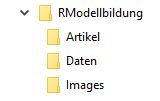
\includegraphics[width=0.20000\textwidth]{Images/Verzeichnisstruktur.JPG}
\caption{Dateistruktur für R-Projekt}
\end{figure}

Die Root kann dabei entweder auf der lokalen Festplatte (C:/..) oder
einem Server, bzw. Cloud (../NextCloud/R Modellbildung/Images) liegen.

Das Anlegen eines R-Projektes wird im RStudio durchgeführt.

\begin{figure}
\centering
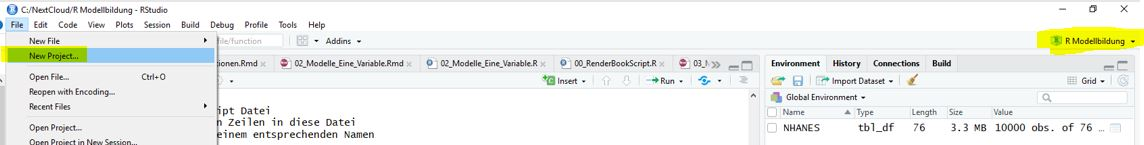
\includegraphics[width=1.00000\textwidth]{Images/Projektdefinieren.JPG}
\caption{R-Projekt definieren}
\end{figure}

Nachdem bereits eine Verzeichnisstruktur definiert wurde, kann man das
Projekt in das bereits definierte Verzeichnis legen (Folge den Schritten
die von RStudio vorgegeben werden). Den Vorteil des projektbasierten
Arbeitens werden wir im Verlauf des Kurses noch näher kennen lernen.

Inhalte, Beispiele und Daten stammen teilweise aus dem Internet, u.a.
(Coursera \protect\hyperlink{ref-CourseRa}{2018}), (DataCamp
\protect\hyperlink{ref-DataCamp}{2018}) und dem Buch (Field
\protect\hyperlink{ref-Field}{2017}).

\section*{Einleitung}\label{einleitung}
\addcontentsline{toc}{section}{Einleitung}

Donald Knuth, einer der Pioniere und bedeutensten Persönlichkeiten in
der Entwicklung von Programmiersprachen, vertrat in seinem Buch Compter
\emph{Programming as an art} (Knuth \protect\hyperlink{ref-Knuth}{2008})
die Auffassung, dass rein wissenschaftliches Arbeiten durch einen
Computer erlernt werden kann (\emph{Science is knowledge which we
understand so well that we can teach it to a computer}). Alle andere
Formen der Datenanalyse bezeichnete er als Kunst.

Neben statistischen Methoden, maschinellem Lernen, diversen
Softwarepaketen und verschiedensten Werkzeugen stehen heutzutage auch
entsprechend leistungsfähige Computer zur Verfügung, um Unmengen von
Daten aufzuzeichnen und zu verarbeiten. Die \emph{Kunst}, Wirklichkeit
in bestmöglicher Form durch ein Modell abzubilden, besteht demnach
darin, die:

\begin{itemize}
\tightlist
\item
  richtigen Fragen zu stellen.
\item
  Daten zu sammeln, mit welchen diese Fragen beantwortet werden können.
\item
  entsprechenden Methoden und Werkzeuge anzuwenden.
\item
  Ergebnisse richtig zu interpretieren.
\item
  Ergebnisse zu vermitteln.
\end{itemize}

In den meisten Fällen ist es nicht möglich, die Wirklichkeit absolut
getreu durch Daten abzubilden. Seit Urzeiten verwendet daher der Mensch
Modelle, um zumindest mit einer Annäherung diese möglichst genau
darzustellen und daraus Rückschlüsse für sonst nicht (oder nur schwer)
zu erklärende Phänome zu ziehen. In einem Artilel beschreibt G. Box (Box
\protect\hyperlink{ref-Box}{1979}) sehr treffend die Eigenschaften von
Modellen:

\begin{quote}
Now it would be very remarkable if any system existing in the real world
could be exactly represented by any simple model. However, cunningly
chosen parsimonious models often do provide remarkably useful
approximations. For example, the law \(P \cdot V = R \cdot T\) relating
pressure P, volume V and temperature T of an ``ideal'' gas via a
constant R is not exactly true for any real gas, but it frequently
provides a useful approximation and furthermore its structure is
informative since it springs from a physical view of the behavior of gas
molecules. For such a model there is no need to ask the question ``Is
the model true?''. If ``truth'' is to be the ``whole truth'' the answer
must be ``No''. The only question of interest is ``Is the model
illuminating and useful?''. --- G. Box
\end{quote}

\section*{\texorpdfstring{Allgemeine Definition des Begriffs
\emph{Modell}}{Allgemeine Definition des Begriffs Modell}}\label{allgemeine-definition-des-begriffs-modell}
\addcontentsline{toc}{section}{Allgemeine Definition des Begriffs
\emph{Modell}}

Allgemein versteht man unter
\href{https://de.wikipedia.org/wiki/Modellbau}{Modellbau} die
Herstellung eines konkreten, dreidimensionalen, physischen Objektes. Der
Prozess der
\href{https://de.wikipedia.org/wiki/Modell\#Modellbildung}{Modellbildung}
abstrahiert dabei mit dem Erstellen eines Modells von der Realität, weil
diese meist zu komplex ist, um sie vollständig abzubilden.

Diese Vollständigkeit wird aber auch gar nicht beabsichtigt, vielmehr
sollen lediglich die wesentlichen Einflussfaktoren identifiziert und
dargestellt werden, die für den realen Prozess und im Modellkontext
bedeutsam sind.

Der Begriff Modell entstand im Italien der Renaissance (italienisch
\emph{modello}), hervorgegangen aus lateinischesn \emph{modulus}, einem
Maßstab in der Architektur. Es wurde bis ins 18. Jahrhundert vorwiegend
in der bildenden Kunst als Fachbegriff verwendet.

In der Umgangssprache wird heutzutage das Wort \emph{Modell} für
unterschiedliche Sachverhalte verwendet. Im naturwissenschaftlichen
Erkenntnisprozess haben Modelle verschiedene Bedeutungen und Funktionen.
Merkmale und Charakteristika, an denen ein Modell eindeutig als Modell
definiert werden kann, existieren nicht (Upmeier
\protect\hyperlink{ref-Upmeier-Krueger-2010}{2010}). Die Bedeutung ist
zudem vom Kontext abhängig. Beim \emph{Modellsein} werden folgende
Aspekte unterschieden (Mahr
\protect\hyperlink{ref-Mahr-Bernd-2008}{2008}):

\begin{itemize}
\tightlist
\item
  Modell \emph{für} etwas sein.
\item
  Modell \emph{von} etwas sein.
\end{itemize}

Dies muss auch bei der Beurteilung eines Modells, also der Frage, ob ein
Modell ein gutes Modell ist, berücksichtigen werden. Hier ist die Frage
des Zwecks des Modells entscheidend. Mahr benennt drei allgemeine
Kriterien zur Beurteilung von Modellen:

\begin{enumerate}
\def\labelenumi{\arabic{enumi}.}
\tightlist
\item
  Das Modell muss die Funktion erfüllen.
\item
  Durch seine Anwendung etwas von dem, wovon es ein Modell ist, zudem
  wofür es ein Modell ist, transportieren.
\item
  Das Modell muss ein Garant von Konsistenz sein.
\end{enumerate}

D.h., dass das Modell garantieren muss, dass es keine Widersprüche
enthält, so dass seine Anwendung nicht notwendig zu Widersprüchen führen
muss. Das Modell muss über eine ausreichende pragmatische Eignung
verfügen und demnach das, wofür oder wovon es ein Modell ist,
ausreichend und angemessen repräsentieren.

Die Hauptfunktion in den Naturwissenschaften ist die Untersuchung und
Interpretation von naturwissenschaftlichen Phänomenen. Ziel ist die
Reduzierung von Komplexität und somit die Erzeugung eines fokussierten
Bildes des zu untersuchenden Objekts. Man kann sagen, dass Modelle den
Blick auf das Wesentliche eines Phänomens oder Gegenstandes lenken
sollen. Das Modell ist somit ein Repräsentant des Originals. Modell und
Original können sich aber im Material, der Dimensionierung und der
Abstraktion unterscheiden. Sie können gegenständlich, bildhaft,
schematisch oder formelhaft sein.

\part*{Teil I:
Begrifflichkeiten}\label{part-teil-i-begrifflichkeiten}
\addcontentsline{toc}{part}{Teil I: Begrifflichkeiten}

\section*{Statistisches Modell}\label{statistisches-modell}
\addcontentsline{toc}{section}{Statistisches Modell}

Ein
\href{https://de.wikipedia.org/wiki/Statistisches_Modell}{statistisches
Modell}, manchmal auch statistischer Raum genannt, ist ein Begriff aus
der mathematischen Statistik, dem Teilbereich der Statistik, der sich
der Methoden der Stochastik und Wahrscheinlichkeitstheorie bedient.
Unter \emph{statistischer Modellbildung} versteht man dabei den Prozess,
ein passendes Modell für die Daten einer Beobachtungsreihe zu finden.

\begin{itemize}
\tightlist
\item
  Als \emph{Prozess} wird die strukturierte und gesteuerte Reihe von
  Arbeitsschritten bezeichnet, welche ein bestimmtes Ergebnis
  hervorbringen.
\item
  \emph{Daten} sind Werte und Beobachtungen, die im Lauf einer
  (statistischen) Erhebung gesammelt werden.
\item
  Eine \emph{Erhebung} ist die Sammlung von Daten einer bestimmten
  Grundgesamtheit zum Zweck der Untersuchung eines speziellen Aspektes.
  Die Daten werden oft nur von einer Stichprobe der Grundgesamtheit
  erhoben. Erhebungen sind in der Forschung weit verbreitet.
\item
  Eine \emph{Stichprobe} ist die Teilmenge einer Grundgesamtheit bei
  einer statistischen Untersuchung, zusammengestellt, um ausgewählte
  Eigenschaften der Gesamtpopulation zu untersuchen.
\end{itemize}

\subsection*{Modellbildung}\label{modellbildung}
\addcontentsline{toc}{subsection}{Modellbildung}

Die Modellbildung abstrahiert mit dem Erstellen eines Modells von der
Realität, weil diese meist zu komplex ist, um sie vollständig
abzubilden. Man unterscheidet dabei:

\begin{itemize}
\item
  \textbf{Strukturelle Modellbildung}: Bei struktureller Modellbildung
  ist die innere Struktur des Systems bekannt, es wird jedoch bewusst
  abstrahiert, modifiziert und reduziert. Man spricht hier von einem
  \textbf{Whitebox-Modell}.
\item
  \textbf{Pragmatische Modellbildung}: Bei pragmatischer Modellbildung
  ist die innere Struktur des Systems unbekannt, es lässt sich nur das
  Verhalten bzw. die Interaktion des Systems beobachten und modellieren.
  Die Hintergründe lassen sich meist nicht oder nur zum Teil verstehen -
  hier spricht man von einem \textbf{Blackbox-Modell}.
\item
  \textbf{Mischformen}: Bei Mischformen sind Teile des Systems bekannt,
  andere wiederum nicht. Nicht alle Wechselwirkungen und Interaktionen
  zwischen Teilkomponenten lassen sich nachvollziehen - hier spricht man
  vom \textbf{Greybox-Modell}. Diese Mischform ist die häufigste, weil
  es aufgrund von Kosten-Nutzen-Überlegungen meist ausreichend ist, das
  System auf diese Weise abzubilden.
\end{itemize}

\subsection*{Kennzeichen eines
Modelles}\label{kennzeichen-eines-modelles}
\addcontentsline{toc}{subsection}{Kennzeichen eines Modelles}

Ein Modell ist im Wesentlichen durch drei Merkmale gekennzeichnet:

\begin{itemize}
\item
  \textbf{Abbildung}: eines natürlichen oder eines künstlichen
  Originals, wobei dieses Original selbst auch wiederum ein Modell sein
  kann.
\item
  \textbf{Verkürzung}: es erfasst im Allgemeinen nicht alle
  Eigenschaften (Attribute) des Originals, sondern nur diejenigen, die
  dem Modellschaffer bzw. Modellnutzer relevant erscheinen. Diese werden
  häufig in Form von aggregierenden Maßzahlen (Parameter) beschrieben.
\item
  \textbf{Pragmatismus}: sind ihren Originalen nicht eindeutig
  zugeordnet. Sie erfüllen ihre Ersetzungsfunktion:

  \begin{itemize}
  \tightlist
  \item
    für bestimmte Subjekte (für wen?)
  \item
    innerhalb bestimmter Zeitintervalle (wann?)
  \item
    unter Einschränkung auf bestimmte gedankliche oder tatsächliche
    Operationen (wozu?).
  \end{itemize}
\end{itemize}

Im übertragenen Sinn ist damit ein statistisches Modell:

\begin{itemize}
\tightlist
\item
  Eine vereinfachte mathematisch-formalisierte Methode, sich der
  Realität anzunähern.
\item
  Die Beschreiben des Zustandes eines Systems vor und nach Änderungen
  äußerer Relationen, nicht jedoch während einer Änderung.
\end{itemize}

Das Ziel ist es herauszufinden, ob man in der Natur auftretende
Phänomene auf allgemein gültige Gesetzmäßigkeiten zurückführen kann. In
der Regel werden Beobachtungen durchgeführt und diese als Daten
aufgezeichnet. In diesen Daten gilt es Muster zu finden, die
Rückschlüsse auf die Mechanismen zulassen, welche dem Phänomen zugrunde
liegen. Auf diese Weise wird ein Modell von der Funktionsweise eines
Phänomens erstellt.

Statistische Modelle finden Verwendung für:

\begin{itemize}
\tightlist
\item
  Annäherung (Approximation)
\item
  Erklärung
\item
  Vorhersage
\end{itemize}

Statistische Modelle sind in fast allen Anwendungsbereichen der
Wissenschaft, aber auch des praktischen Lebens zu finden, wie z.B.:

\begin{itemize}
\tightlist
\item
  Bei Wettervorhersagen.
\item
  In der Finanzmarktanalyse.
\item
  In der Industrie und Gewerbe.
\item
  Bei Wahlprognosen, Meinungsumfragen.
\item
  In der Informationstechnologie.
\item
  etc.
\end{itemize}

\subsubsection*{Zyklus der
Modellbildung}\label{zyklus-der-modellbildung}
\addcontentsline{toc}{subsubsection}{Zyklus der Modellbildung}

Das Bilden von statistischen Modellen ist ein iterativer Vorgang,
welcher durchaus mehrere zyklische Entwicklungsschritte beinhalten kann.

\begin{figure}
\centering
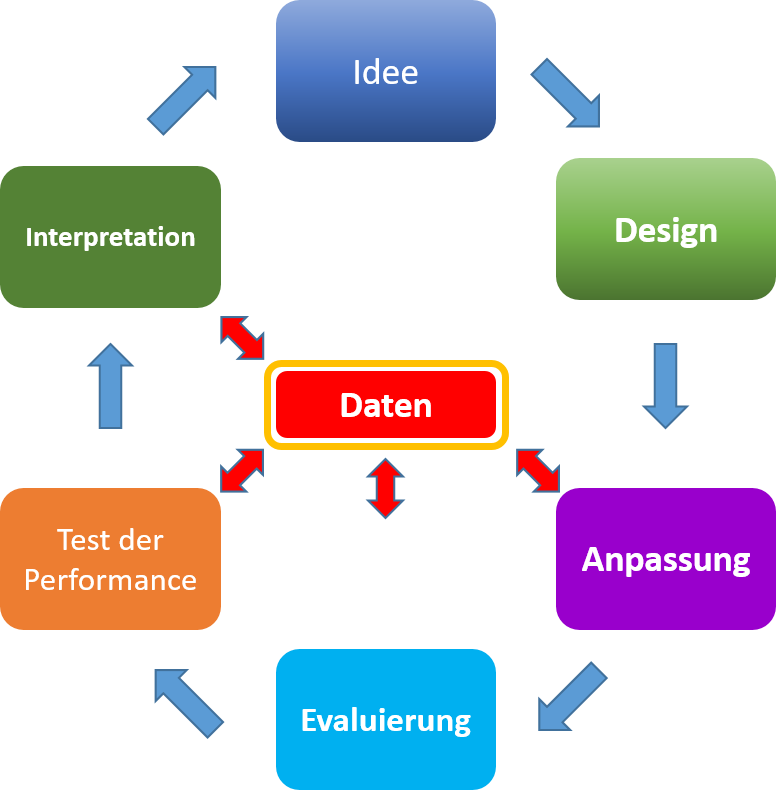
\includegraphics[width=0.40000\textwidth]{Images/ZyklusModellbildung.PNG}
\caption{\textbf{Abbildung 1}: Zyklus der Modellbildung}
\end{figure}

\subsection*{Grundlagen der statistischen
Modellbildung}\label{grundlagen-der-statistischen-modellbildung}
\addcontentsline{toc}{subsection}{Grundlagen der statistischen
Modellbildung}

Grundlage ist eine entsprechende Fragestellung, die auf theoretischen
Grundlagen basiert und möglichst präzise formuliert werden soll. Bei den
Daten, die zur Beantwortung der Fragestellung geeignet sind, sollte man
speziell achten auf:

\begin{itemize}
\tightlist
\item
  woher Sie kommen.
\item
  was und wie Sie ein erhobenes/gemessenes Objekt abbilden.
\end{itemize}

Charakteristiken von guten Fragen sind:

\begin{itemize}
\tightlist
\item
  \textbf{Interessant für andere}: wie z.B. für Mitarbeiter,
  wissenschaftliche Gemeinschaft, Geldgeber, Allgemeinheit?
\item
  \textbf{Noch nicht beantwortet}: wurde die Fragestellung bereits
  bearbeitet/beantwortet? Das erfordert eine intensive
  Auseinandersetzung mit dem Thema (Literaturrecherche,
  Kongressbeiträge, etc.).
\item
  \textbf{Sinnvoll}: kann durch die Beantwortung eine Erklärung gefunden
  werden, wie etwas funktioniert?
\item
  \textbf{Beantwortbarkeit}: kann die Fragestellung überhaupt
  beantwortet werden?
\item
  \textbf{Spezifisch}: wie präzise ist die Fragestellung? Gesundes Essen
  führt zu besserer Gesundheit ist weniger präzise wie z.B. 5 Mal am Tag
  Früchte und Gemüse führt zu einer geringeren Wahrscheinlichkeit an
  Atemwegserkrankungen zu erkranken.
\end{itemize}

Bei den Qualitätskriterien für Daten ist folgendes zu beachten:

\begin{itemize}
\tightlist
\item
  \textbf{Korrektheit} \(\rightarrow\) müssen mit der Realität
  übereinstimmen.
\item
  \textbf{Konsistenz} \(\rightarrow\) dürfen in sich und zu anderen
  Datensätzen keine Widersprüche aufweisen.
\item
  \textbf{Zuverlässigkeit} \(\rightarrow\) Entstehung der Daten muss
  nachvollziehbar sein.
\item
  \textbf{Vollständigkeit} \(\rightarrow\) muss alle notwendigen
  Attribute enthalten.
\item
  \textbf{Genauigkeit} \(\rightarrow\) müssen in der jeweils geforderten
  Exaktheit vorliegen (Beispiel: Nachkommastellen).
\item
  \textbf{Aktualität} \(\rightarrow\) müssen jeweils dem aktuellen
  Zustand der abgebildeten Realität entsprechen.
\item
  \textbf{Relevanz} \(\rightarrow\) Der Informationsgehalt muss den
  jeweiligen Informationsbedarf erfüllen.
\item
  \textbf{Einheitlichkeit} \(\rightarrow\) Die Informationen müssen
  einheitlich strukturiert sein.
\item
  \textbf{Eindeutigkeit} \(\rightarrow\) muss eindeutig interpretierbar
  sein.
\item
  \textbf{Verständlichkeit} \(\rightarrow\) müssen in ihrer
  Begrifflichkeit und Struktur mit den Vorstellungen der Fachbereiche
  übereinstimmen.
\item
  \textbf{Redundanzfreiheit}: Innerhalb der Datensätze sollen/dürfen
  keine Dubletten vorkommen.
\end{itemize}

Aus der Testtheorie sind in auch die Gütekriterien
(\emph{Testgütekriterien}) der empirischen Forschung für die
statistische Modellbildung anzuwenden. Diese sind:

\begin{itemize}
\tightlist
\item
  \textbf{Reliabilität}: Indikator für die Replizierbarkeit der
  Ergebnisse. Fragen müssen z.B. so eindeutig formuliert sein, dass sie
  nicht höchst unterschiedlich verstanden werden können.
\item
  \textbf{Validität}: wenn die gewählten Indikatoren, Fragen und
  Antwortmöglichkeiten wirklich und präzise das messen, was gemessen
  werden soll.
\item
  \textbf{Objektivität}: wenn die Wahl der Messenden, InterviewerInnen,
  PrüferInnen keinen Einfluss auf die Ergebnisse hat.
\end{itemize}

Bei der Analyse und Interpretation der Daten unterscheidet man:

\begin{itemize}
\tightlist
\item
  \textbf{Deskriptiv}: beschreibend (innerhalb Daten)
\item
  \textbf{Explorativ}: Hypothesen generierend (innerhalb Daten)
\item
  \textbf{Inferentiell}: Statement über etwas, was nicht beobachtet
  wird, also aus den erhobenen Daten auf die Ursachen zu schliessen, die
  die Daten erzeugt haben könnten (außerhalb der Daten).
\item
  \textbf{Prädiktiv}: Vorhersage für Werte die noch nicht beobachtet
  wurden (außerhalb der Daten)
\item
  \textbf{Korrelativ}: Beschreibung der Zusammenhäng zwischen
  Beobachtungen (innerhalb und außerhalb der Daten).
\item
  \textbf{Mechanistisch}: nicht nur die Frage ob ein Zusammenhang
  besteht, sondern wie und warum der Zusammenhang besteht ist von
  Interesse.
\end{itemize}

\subsubsection*{Deskriptive Statistik}\label{deskriptive-statistik}
\addcontentsline{toc}{subsubsection}{Deskriptive Statistik}

Die deskriptive Statistik hat zum Ziel, empirische Daten durch Tabellen,
Kennzahlen (auch: Maßzahlen oder Parameter) und Grafiken übersichtlich
darzustellen und zu ordnen.

Die Methoden der deskriptiven Statistik umfassen:

\begin{itemize}
\tightlist
\item
  Tabellen
\item
  Diagramme
\item
  Parameter (Maßzahlen, Kennzahlen, Kennwerte)

  \begin{itemize}
  \tightlist
  \item
    Lagemaßen: Maße der zentralen Tendenz, wie z.B. Mittelwerte, Median,
    Modus.
  \item
    Streuungsmaße: für die Variabilität (Dispersion), wie z.B. Range,
    Varianz, Standardabweichung, Standardfehler.
  \item
    Zusammenhangsmaße: wie z.B. die Korrelation.
  \end{itemize}
\end{itemize}

Die deskriptive Statistik ist ein zentrales Element jeder formalen
Analyse von Daten, hat jedoch in ihrer Eigenschaft folgende
Einschränkungen:

\begin{itemize}
\tightlist
\item
  liefert keine Aussagen zu einer über die untersuchten Fälle
  hinausgehenden Grundgesamtheit .
\item
  Es ist keine Überprüfung von Hypothesen möglich.
\item
  Verwendet keine stochastischen Modelle (Grundlage der induktiven
  Statistik).
\item
  getroffenen Aussagen können nicht durch Fehlerwahrscheinlichkeiten
  abgesichert werden.
\end{itemize}

\subsubsection*{Explorative Datenanalyse
(EDA)}\label{explorative-datenanalyse-eda}
\addcontentsline{toc}{subsubsection}{Explorative Datenanalyse (EDA)}

Die explorative Datenanalyse/Statistik hat zum Ziel, bisher unbekannte
Strukturen und Zusammenhänge in den Daten zu finden und hierdurch neue
Hypothesen zu generieren. Diese auf Stichprobendaten beruhenden
Hypothesen können dann im Rahmen der schließenden Statistik mittels
wahrscheinlichkeitstheoretischer Methoden auf ihre Allgemeingültigkeit
untersucht werden.

Die Methoden der explorativen Statistik sind meist identisch mit denen
der deskriptiven Statistik, unterscheiden sich aber bezüglich der
\emph{Ziele der Analyse}. Bei der EDA sollten vor allem die
nachfolgenden Fragen geklärt werden:

\begin{itemize}
\tightlist
\item
  Haben wir die richtigen Daten zur Beantwortung der Fragestellung?
\item
  Brauchen wir mehr Daten?
\item
  Müssen wir die Fragestellung verfeinern?
\item
  Was kann aus den vorliegenden Daten abgeleitet werden?
\end{itemize}

Die Ziele der EDA sind:

\begin{itemize}
\tightlist
\item
  bisher unbekannte Strukturen und Zusammenhänge in den Daten zu finden.
\item
  Annahmen (Hypothesen) über die Ursache und den Grund der beobachteten
  Daten zu bilden.
\item
  Annahmen einzuschätzen, worauf statistische Inferenz basieren kann.
\item
  Die Auswahl von passenden statistischen Werkzeugen und Techniken zu
  unterstützen.
\item
  Eine Basis für die weitere Datensammlung durch Umfragen oder Design
  von Experimenten bereitzustellen.
\end{itemize}

Speziell in Bezug auf die erforderliche Stichprobengröße sollte vor
Begin der Datenerhebung die mindest notwendigen Fallzahlen (optimaler
Stichprobenumfang) bestimmt werden, der für den Nachweise praktisch
bedeutsamer Effekte notwendig ist. Sowohl in R als auch in diversen
Anwednungen gibt es die Möglichkeit, diese optimale Stichprobengröße a
priori zu bestimmen.

Voraussetzung dafür sind jedoch Kenntnisse über den zu erwartenden
Effekt. Dieser kann entweder durch einer Meta-Analyse oder durch
entsprechende Erfahrungswerte bestimmt werden. Zusätzlich ist dann noch
die Irrtumswahrscheinlichkeit, die gewünschte Teststärke und die
verwendete statistischen Methode festzulegen. Je größer eine Stichprobe
ist, desto genauer werden auch die daraus abgeleiteten Kennwerte und
Teststatistiken Auskunft über die in der Population gültigen Werte
liefern. Aus praktischen/finanziellen/zeitlichen Gründen wird man jedoch
i.A. danach trachten, eine möglichst kleine Stichprobe zu erheben.
Generell lassen sich diesbezüglich folgende Aussagen treffen:

\begin{itemize}
\tightlist
\item
  bei großen Stichproben werden auch kleine Effekte im statistischen
  Sinn signifikant (damit ist nicht gesagt, dass auch eine praktische
  Signifikanz des Effektes vorliegt).
\item
  bei kleinen Stichproben wird ein kleiner Effekt oft statistisch nicht
  signifikant. Wenn doch, ist das oft nur ein Zufallsergebnis und kann
  i.A. nicht reproduziert werden.
\item
  eine sorgfältige Stichprobenplanung geht mit einer intensiven
  inhaltlichen Auseinandersetzung einher. Der Vorteil dieser Planung
  liegt also nicht nur in der Wahrscheinlichkeit, einen vorhandenen
  Effekt auch stastisch absichern zu können, sondern vor allem auch
  darin, dass eventuell schon beantwortete Fragen rechtzeitig entdeckt
  werden!
\end{itemize}

\subsubsection*{Inferenzstatistik}\label{inferenzstatistik}
\addcontentsline{toc}{subsubsection}{Inferenzstatistik}

Bei der inferentiellen Statistik wird eine Zufallsstichprobe aus einer
Grundgesamtheit entnommen, um Rückschlüsse auf die Grundgesamtheit zu
ziehen und diese zu beschreiben. Weitere Begriffe sind:

\begin{itemize}
\tightlist
\item
  analytische Statistik
\item
  inferenzielle Statistik
\item
  induktive Statistik
\item
  schließende Statistik
\end{itemize}

Die inferentielle Statistik ist in den Situationen nützlich, in denen es
nur schwer oder gar nicht möglich ist, eine vollständige Grundgesamtheit
zu untersuchen. Wesentliche Merkmale der Inferenzstatistik sind:

\begin{itemize}
\tightlist
\item
  trifft Wahrscheinlichkeitsaussagen über Populationswerte.
\item
  Daten werden in Form von (Zufalls-) Stichproben aus der
  Grundgesamtheit entnommen.
\item
  Signifikanztests und Intervalleschätzungen bieten die
  Entscheidungsgrundlage hinsichtlich der postulierten Hypothesen.
\end{itemize}

\subsubsection*{Prädiktive Statistik}\label{pradiktive-statistik}
\addcontentsline{toc}{subsubsection}{Prädiktive Statistik}

Prädikative Statistik (predictive analytics) verwendet (historische)
Daten, um zukünftige Ereignisse vorherzusagen. Im Allgemeinen werden
vorliegende (historische) Daten verwendet, um ein mathematisches
(prädiktives Modell) Modell zu erstellen. Dieses Modell soll bestmöglich
wichtige Trends in den Daten erfassen.

Dieses wird dann auf aktuelle Daten angewendet, um zukünftige Ereignisse
vorherzusagen, oder um Aktionen vorzuschlagen, mit denen optimale
Ergebnisse erreicht werden können. Vor allem in den letzten Jahren hat
diese Form der Statistik in den Bereichen von Big Data und Machine
Learning sehr an Bedeutung gewonnen.

\subsubsection*{Mechanististische
Statistik}\label{mechanististische-statistik}
\addcontentsline{toc}{subsubsection}{Mechanististische Statistik}

Zusammenhängen zwischen mehreren Variablen mit gleichzeitiger
Interpretation der Kausalitäten werden häufig mit Hilfe eines
Strukturgleichungsmodells (SEM\footnote{\emph{S}tructural
  \emph{E}quation \emph{M}odeling}) analysiert. Dabei handelt es sich um
ein statistisches Modell, das das Schätzen und Testen korrelativer
Zusammenhänge zwischen abhängigen Variablen und unabhängigen Variablen
sowie den verborgenen Strukturen dazwischen erlaubt.

Eine Besonderheit von Strukturgleichungsmodellen ist das Überprüfen
latenter (nicht direkt beobachtbarer) Variablen. Spezialfälle von
Strukturgleichungsmodellen sind:

\begin{itemize}
\tightlist
\item
  Pfadanalyse
\item
  Faktorenanalyse
\item
  Regressionsanalyse
\end{itemize}

Ein Strukturgleichungsmodell stellt wiederum einen Spezialfall eines
sogenannten Kausalmodells dar.

\part*{Teil II: Modelle mit einer
Variablen}\label{part-teil-ii-modelle-mit-einer-variablen}
\addcontentsline{toc}{part}{Teil II: Modelle mit einer
Variablen}

\section*{Datensatz}\label{datensatz}
\addcontentsline{toc}{section}{Datensatz}

Betrachten wir zunächst einen einfachen Datensatz aus dem Projekt MOSAIC
Data Sets (Paket mosaicData, \textbf{CPS85})\footnote{\href{http://mosaic-web.org/}{Project
  MOSAIC}, is a community of educators working to develop a new way to
  introduce mathematics, statistics, computation and modeling to
  students in colleges and universities.}.

Diese Datei beinhaltet \emph{N =} \texttt{534} Beobachtungen und \emph{k
=} \texttt{11} Variablen, deren Namen in folgender Tabelle nochmals
separat angeführt sind:

\begin{tabular}{r|l}
\hline
LNr & Variablenname\\
\hline
1 & wage\\
\hline
2 & educ\\
\hline
3 & race\\
\hline
4 & sex\\
\hline
5 & hispanic\\
\hline
6 & south\\
\hline
7 & married\\
\hline
8 & exper\\
\hline
9 & union\\
\hline
10 & age\\
\hline
11 & sector\\
\hline
\end{tabular}

Angenommen Sie müssten auf Basis der vorliegenden Daten für eine Person
das durchschnittliche Einkommen (\emph{wage}) schätzen, ohne dabei
andere Variablen zu berücksichtigen. Welchen Wert würden Sie wählen?

\section*{Deskriptive Statistik}\label{deskriptive-statistik-1}
\addcontentsline{toc}{section}{Deskriptive Statistik}

Bevor man diese Frage beantwortet, sollte man sich die deskriptive
Statistik der entsprechenden Variablen genauer ansehen. In der
vorliegenden Fragestellung handelt es sich um eine intervallskalierte
Variable, daher ist die Betrachtung der Kennwerte für zentrale Tendenzen
(Mittelwert, Median, Modus, Minimum, Maximum und Range), der Dispersion
(Varianz, Standardabweichung, Quartile, Standardfehler,
Konfidenzintervalle, Schiefe und Kurtosis), sowie die Darstellung der
Verteilung in einem Histogramm sehr hilfreich.

Unter bestimmten Voraussetzungen, eignet sich der Mittelwert als bester
Schätzer (bzw. als einfachste Modellvorstellung). Bevor man sich jedoch
der Auswertung von Daten widmet, ist es sehr empfehlenswert die
zugrundeliegende Datenstruktur zu analysieren und auch zu dokumentieren.
Im nachfolgenden Kapitel wird ein sehr nützliches Paket für genau diese
Analyse kurz vorgestellt.

\hypertarget{codebooks-in-r}{\subsection*{Codebooks in
R}\label{codebooks-in-r}}
\addcontentsline{toc}{subsection}{Codebooks in R}

In R hat man die Möglichkeit, mit Hilfe des Pakets \emph{codebook} eine
genaue Beschreibung der Daten (inklusive einer deskriptiven Statistik
für jede Variable) zu erstellen. Für den vorliegenden Datensatz wurde
auszugsweise eines erstellt, welches in Kapitel
\protect\hyperlink{codebook-cps85}{Codebook CPS85} zu finden ist.

\subsubsection*{Tabellen}\label{tabellen}
\addcontentsline{toc}{subsubsection}{Tabellen}

Im Codebook werden neben den deskriptiven Kennwerten (für kategorielle
Variablen) Häufigkeitstabellen angegeben. Wir wollen uns daher einen
kurzen Überblick über Häufigkeitstabellen in R verschaffen. Kopiere den
nachfolgenden Code in den Editor und führe in aus. Diskutiere die
Ergebnisse.

\begin{Shaded}
\begin{Highlighting}[]
\NormalTok{  Income <-}\StringTok{ }\NormalTok{CPS85}\OperatorTok{$}\NormalTok{wage}
  \KeywordTok{library}\NormalTok{(pastecs)}
    \KeywordTok{kable}\NormalTok{(}\KeywordTok{stat.desc}\NormalTok{(Income))}
    \CommentTok{# DT::datatable(data.frame(stat.desc(Income)))}
  \KeywordTok{library}\NormalTok{(psych)}
    \KeywordTok{kable}\NormalTok{(}\KeywordTok{describe}\NormalTok{(Income))}
    \CommentTok{# DT::datatable(data.frame(describe(Income)))}

  \CommentTok{# Häufigkeitstabellen}
\NormalTok{  SR  <-}\StringTok{ }\KeywordTok{table}\NormalTok{(CPS85}\OperatorTok{$}\NormalTok{sex, CPS85}\OperatorTok{$}\NormalTok{race)}
  \KeywordTok{kable}\NormalTok{(SR)}
\NormalTok{  SRM <-}\StringTok{ }\KeywordTok{table}\NormalTok{(CPS85}\OperatorTok{$}\NormalTok{sex, CPS85}\OperatorTok{$}\NormalTok{race, CPS85}\OperatorTok{$}\NormalTok{married)}
  \KeywordTok{kable}\NormalTok{(SRM)}
  \CommentTok{# Häufigkeitstabellen mit Randsummen}
\NormalTok{  x0 <-}\StringTok{ }\KeywordTok{addmargins}\NormalTok{(}\KeywordTok{table}\NormalTok{(CPS85}\OperatorTok{$}\NormalTok{sex, CPS85}\OperatorTok{$}\NormalTok{race))}
  \KeywordTok{kable}\NormalTok{(x0)}
  \CommentTok{# Häufigkeitstabellen in Prozent}
\NormalTok{  x1 <-}\StringTok{ }\KeywordTok{addmargins}\NormalTok{(}\KeywordTok{round}\NormalTok{(}\DecValTok{100}\OperatorTok{*}\KeywordTok{prop.table}\NormalTok{(}\KeywordTok{table}\NormalTok{(CPS85}\OperatorTok{$}\NormalTok{sex, CPS85}\OperatorTok{$}\NormalTok{race)), }\DecValTok{2}\NormalTok{))}
  \KeywordTok{kable}\NormalTok{(x1)}
\end{Highlighting}
\end{Shaded}

\section*{Mittelwerts-Modell}\label{mittelwerts-modell}
\addcontentsline{toc}{section}{Mittelwerts-Modell}

Wie bereits erwähnt, wäre unter bestimmten Voraussetzungen
(Verteilungseigenschaften) der Mittelwert ein guter Schätzer, da dieser
die folgende Eigenschaft besitzt:

\begin{itemize}
\tightlist
\item
  Die Summe der quadrierten Abweichungen der Beobachtungswerte \(x_i\)
  von einem beliebigen Punkt \(m\) wird minimal, wenn dieser Punkt
  \(m = \bar{x}\), also der arithmetische Mittelwert ist!
\end{itemize}

Formal berechnet sich das arithmetische Mittel:

\begin{equation} 
  \bar{x} = \frac{1}{N} \sum_{i=1}^{N} x_i
  \label{eq:MW}
\end{equation}

Die Aussagekraft des arithmetischen Mittels beschränkt sich jedoch ganz
wesentlich, wenn nicht weitere Kennwerte der Daten bekannt sind. Vor
allem ist es von Interesse, die Streung (Variabilität) der Werte um den
Mittelwert zu kennen. Diese wird durch das Streuungsmaß, welches als
durchschnittliche Abweichung der Messwerte um den Mittelwert gesehen
werden kann, beschrieben:

\begin{equation} 
  s = \sqrt{\sum_{i=1}^{N} (x_i \frac{x_i - \bar{x})^2}{N-1}}
  \label{eq:SD}
\end{equation}

\subsection*{\texorpdfstring{Modell \emph{idealer}
Daten}{Modell idealer Daten}}\label{modell-idealer-daten}
\addcontentsline{toc}{subsection}{Modell \emph{idealer} Daten}

Betrachten wir zunächst einen Datensatz, in dem das Gehalt (\emph{wage})
symmetrisch und in Form einer Glockenkurve gegeben ist. Kopiere den
nachfolgenden Code in dein R-Script und führe diesen dann aus.

\begin{Shaded}
\begin{Highlighting}[]
  \KeywordTok{options}\NormalTok{(}\DataTypeTok{digits =} \DecValTok{2}\NormalTok{)}
\NormalTok{  DF      <-}\StringTok{ }\NormalTok{CPS85}
  \KeywordTok{set.seed}\NormalTok{(}\DecValTok{825}\NormalTok{)}
\NormalTok{  DF}\OperatorTok{$}\NormalTok{wage <-}\StringTok{ }\KeywordTok{rnorm}\NormalTok{(}\DataTypeTok{n =} \KeywordTok{nrow}\NormalTok{(DF), }\DataTypeTok{mean =} \DecValTok{8}\NormalTok{, }\DataTypeTok{sd =} \FloatTok{2.3}\NormalTok{)}
\NormalTok{  Income  <-}\StringTok{ }\NormalTok{DF}\OperatorTok{$}\NormalTok{wage}
  
  \CommentTok{# Kennwerte berechnen}
\NormalTok{  MW <-}\StringTok{ }\KeywordTok{mean}\NormalTok{(Income)}
\NormalTok{  SD <-}\StringTok{ }\KeywordTok{sd}\NormalTok{(Income)}
\NormalTok{  MD <-}\StringTok{ }\KeywordTok{median}\NormalTok{(Income)}
\NormalTok{  RA <-}\StringTok{ }\KeywordTok{range}\NormalTok{(Income)}
  \CommentTok{# Daten anzeigen}
  \CommentTok{# p1 <- hist(Income)}
  \CommentTok{# p2 <- boxplot(Income)}
  
  \CommentTok{# starke Abweichungen entfernen}
\NormalTok{  TrimmedIncome <-}\StringTok{ }\NormalTok{Income[}\OperatorTok{!}\NormalTok{Income }\OperatorTok\StringTok{ }\KeywordTok{boxplot.stats}\NormalTok{(Income)}\OperatorTok{$}\NormalTok{out]}
  \CommentTok{# Kennwerte berechnen}
\NormalTok{  MW_T <-}\StringTok{ }\KeywordTok{mean}\NormalTok{(TrimmedIncome)}
\NormalTok{  SD_T <-}\StringTok{ }\KeywordTok{sd}\NormalTok{(TrimmedIncome)}
\NormalTok{  MD_T <-}\StringTok{ }\KeywordTok{median}\NormalTok{(TrimmedIncome)}
\NormalTok{  RA_T <-}\StringTok{ }\KeywordTok{range}\NormalTok{(TrimmedIncome)}
  \CommentTok{# Daten anzeigen}
  \CommentTok{# p3   <- hist(TrimmedIncome)}
  \CommentTok{# p4   <- boxplot(TrimmedIncome)}
\end{Highlighting}
\end{Shaded}

Die Ergebnisse der statistischen Kennwerte \(\bar{x}\) = (8.0952214),
\(med\) = (8.2289139), \(sd\) = (2.3218623) und vor allem (das hier
nicht angezeigte) angezeigte Histogramm lassen vermuten, dass der
Mittelwert als \emph{Modell} durchaus geeignet ist. Vor allem wenn man
noch durch \emph{Beschneidung (trim)} der Daten die kleinsten und
größten Werte entfernt, nehmen der Mittelwert \(\bar{x}_{trim}\) =
8.1089335 und Median \(med_{trim}\) = 8.2306598 den gleichen Wert ein.

\subsection*{\texorpdfstring{Modell \emph{schiefer}
Daten}{Modell schiefer Daten}}\label{modell-schiefer-daten}
\addcontentsline{toc}{subsection}{Modell \emph{schiefer} Daten}

Um die Eigenschaften des Mittelwertes bei vorliegen von starken
Abweichungen in den Daten noch besser zu verdeutlichen, verwenden wir
einerseits die Originaldaten (welche für sich schon schiefverteilt sind)
und setzen zusätzlich bei 50 zufällig gewählten Personen das Einkommen
drastisch hinauf. Kopiere den folgenden Code ins RStudio und führe
diesen dann aus.

\begin{Shaded}
\begin{Highlighting}[]
\NormalTok{  IncomeNew     <-}\StringTok{ }\NormalTok{CPS85}\OperatorTok{$}\NormalTok{wage}
\NormalTok{  ID            <-}\StringTok{ }\KeywordTok{sample}\NormalTok{(}\DecValTok{1}\OperatorTok{:}\DecValTok{534}\NormalTok{, }\DecValTok{50}\NormalTok{)}
\NormalTok{  IncomeNew[ID] <-}\StringTok{ }\NormalTok{IncomeNew[ID] }\OperatorTok{+}\StringTok{ }\DecValTok{18}
\end{Highlighting}
\end{Shaded}

\hypertarget{aufgabenstellung-1}{\subsubsection*{Aufgabenstellung
1}\label{aufgabenstellung-1}}
\addcontentsline{toc}{subsubsection}{Aufgabenstellung 1}

Berechne für die neuen Daten folgende Kennwerte und zeichne sowohl ein
Histogramm, als auch einen Boxplot.

\begin{itemize}
\tightlist
\item
  Mittelwert
\item
  Standardabweichung
\item
  Median
\item
  Range
\item
  Getrimmten Mittelwert, wobei jeweils 10\% der Daten vom unteren und
  oberen Wertebereich unberücksichtigt bleiben sollen.
\end{itemize}

Diskutiere die Ergebnisse. Die Lösung zu diesen Aufgaben findest du in
\protect\hyperlink{aufgabe_1}{Lösung Aufgabe 1}.

\subsubsection*{Graphische Darstellung}\label{graphische-darstellung}
\addcontentsline{toc}{subsubsection}{Graphische Darstellung}

Zur Veranschaulichung von Verteilungseigenschaften einer Variablen
eignen sich vor allem Histogramme, Boxplots und Q-Q-Plots. In
Kombination mit den entsprechenden Tabellen, können bereits durch die
einfache deskriptive Statistik wertvolle Aussagen über die statistischen
Eigenschaften der Daten gewonnen werden. Kopiere den folgenden Code ins
RStudio und führe diesen dann aus. Diskutiere die Ergebnisse.

\begin{Shaded}
\begin{Highlighting}[]
  \CommentTok{# Histogramme und Density-Plots}
\NormalTok{  p1 <-}\StringTok{ }\KeywordTok{ggplot}\NormalTok{(CPS85, }\KeywordTok{aes}\NormalTok{(}\DataTypeTok{x =}\NormalTok{ wage)) }\OperatorTok{+}\StringTok{ }\KeywordTok{geom_histogram}\NormalTok{()}
\NormalTok{  p2 <-}\StringTok{ }\KeywordTok{ggplot}\NormalTok{(CPS85, }\KeywordTok{aes}\NormalTok{(}\DataTypeTok{x =}\NormalTok{ age)) }\OperatorTok{+}\StringTok{ }\KeywordTok{geom_histogram}\NormalTok{(}\DataTypeTok{binwidth =} \DecValTok{4}\NormalTok{)}
\NormalTok{  p3 <-}\StringTok{ }\KeywordTok{ggplot}\NormalTok{(CPS85, }\KeywordTok{aes}\NormalTok{(}\DataTypeTok{x =}\NormalTok{ exper)) }\OperatorTok{+}\StringTok{ }\KeywordTok{geom_density}\NormalTok{()}
  \CommentTok{# Boxplots}
\NormalTok{  x1 <-}\StringTok{ }\NormalTok{mosaic}\OperatorTok{::}\KeywordTok{mean_}\NormalTok{(wage }\OperatorTok{~}\StringTok{ }\NormalTok{sex, }\DataTypeTok{data =}\NormalTok{ CPS85)}
\NormalTok{  x2 <-}\StringTok{ }\NormalTok{mosaic}\OperatorTok{::}\KeywordTok{sd}\NormalTok{(wage }\OperatorTok{~}\StringTok{ }\NormalTok{sex, }\DataTypeTok{data =}\NormalTok{ CPS85)}
\NormalTok{  x3 <-}\StringTok{ }\NormalTok{mosaic}\OperatorTok{::}\KeywordTok{quantile}\NormalTok{(wage }\OperatorTok{~}\StringTok{ }\NormalTok{sex, }\DataTypeTok{data =}\NormalTok{ CPS85)}
\NormalTok{  x4 <-}\StringTok{ }\NormalTok{mosaic}\OperatorTok{::}\KeywordTok{favstats}\NormalTok{(wage }\OperatorTok{~}\StringTok{ }\NormalTok{sex, }\DataTypeTok{data =}\NormalTok{ CPS85)}
\NormalTok{  x5 <-}\StringTok{ }\KeywordTok{gf_boxplot}\NormalTok{(wage }\OperatorTok{~}\StringTok{ }\NormalTok{sex, }\DataTypeTok{data =}\NormalTok{ CPS85)}
\NormalTok{  x6 <-}\StringTok{ }\KeywordTok{gf_point}\NormalTok{(wage }\OperatorTok{~}\StringTok{ }\NormalTok{sex, }\DataTypeTok{data =}\NormalTok{ CPS85)}
  \CommentTok{# Q-Q Plots}
  \KeywordTok{qqnorm}\NormalTok{(CPS85}\OperatorTok{$}\NormalTok{wage, }\DataTypeTok{pch =} \DecValTok{1}\NormalTok{, }\DataTypeTok{frame =} \OtherTok{FALSE}\NormalTok{)}
  \KeywordTok{qqline}\NormalTok{(CPS85}\OperatorTok{$}\NormalTok{wage, }\DataTypeTok{col =} \StringTok{"steelblue"}\NormalTok{, }\DataTypeTok{lwd =} \DecValTok{2}\NormalTok{)}
\end{Highlighting}
\end{Shaded}

\subsubsection*{Bemerkung Ausreißer}\label{bemerkung-ausreier}
\addcontentsline{toc}{subsubsection}{Bemerkung Ausreißer}

Eine der häufigsten Ursachen für Verzerrungen in den
Verteilungseigenschaften einer Variablen sind Ausreißer. Die Behandlung
von Ausreißern ist ein eigenes und heftig diskutiertes Thema in der
Statistik. Eine (wenngleich nicht unbedenkliche) Methode ist das bereits
verwendete \emph{Trimmen} der Daten. Nachfolgendes Beispiel zeigt eine
weitere Möglichkeit\footnote{wir haben bereits bei der
  Mittelwertsfunktion \emph{mean()} das Argument \emph{trim}
  kennengelernt.}, Ausreißer aus einer Analyse zu entfernen. Es sei an
dieser Stelle nochmals explizit darauf hingewiesen, dass ein beliebiges
Weglassen von \emph{störenden} Werten durchaus bedenklich ist und
eigentlich nur im Sinne einer explorativen Analyse von Daten (was wäre,
wenn die Daten keine Ausreißer hätten?) gerechtfertigt werden kann!
Kopiere den folgenden Code ins RStudio und führe diesen dann aus.
Diskutiere die Ergebnisse.

\begin{Shaded}
\begin{Highlighting}[]
  \CommentTok{# panderOptions("table.split.table", 120)}
  \CommentTok{# pander(head(CPS85), style = "rmarkdown")}
\NormalTok{  MW_Wage    <-}\StringTok{ }\KeywordTok{mean}\NormalTok{(CPS85}\OperatorTok{$}\NormalTok{wage, }\DataTypeTok{na.rm =} \OtherTok{TRUE}\NormalTok{)}
\NormalTok{  Med_Wage   <-}\StringTok{ }\KeywordTok{median}\NormalTok{(CPS85}\OperatorTok{$}\NormalTok{wage, }\DataTypeTok{na.rm =} \OtherTok{TRUE}\NormalTok{)}
\NormalTok{  SD_Wage    <-}\StringTok{ }\KeywordTok{sd}\NormalTok{(CPS85}\OperatorTok{$}\NormalTok{wage, }\DataTypeTok{na.rm =} \OtherTok{TRUE}\NormalTok{)}
\NormalTok{  CPS85_}\DecValTok{1}\NormalTok{    <-}\StringTok{ }\NormalTok{CPS85[}\OperatorTok{!}\NormalTok{CPS85}\OperatorTok{$}\NormalTok{wage }\OperatorTok\StringTok{ }\KeywordTok{boxplot.stats}\NormalTok{(CPS85}\OperatorTok{$}\NormalTok{wage)}\OperatorTok{$}\NormalTok{out,]}
\NormalTok{  MW_Wage_}\DecValTok{1}\NormalTok{  <-}\StringTok{ }\KeywordTok{mean}\NormalTok{(CPS85_}\DecValTok{1}\OperatorTok{$}\NormalTok{wage, }\DataTypeTok{na.rm =} \OtherTok{TRUE}\NormalTok{)}
\NormalTok{  Med_Wage_}\DecValTok{1}\NormalTok{ <-}\StringTok{ }\KeywordTok{median}\NormalTok{(CPS85_}\DecValTok{1}\OperatorTok{$}\NormalTok{wage, }\DataTypeTok{na.rm =} \OtherTok{TRUE}\NormalTok{)}
\NormalTok{  SD_Wage_}\DecValTok{1}\NormalTok{  <-}\StringTok{ }\KeywordTok{sd}\NormalTok{(CPS85_}\DecValTok{1}\OperatorTok{$}\NormalTok{wage, }\DataTypeTok{na.rm =} \OtherTok{TRUE}\NormalTok{)}
  \CommentTok{# Modell0_Graph_1 ----}
  \KeywordTok{ggplot}\NormalTok{(CPS85, }\KeywordTok{aes}\NormalTok{(}\DataTypeTok{x =}\NormalTok{ wage)) }\OperatorTok{+}
\StringTok{    }\KeywordTok{geom_histogram}\NormalTok{(}\KeywordTok{aes}\NormalTok{(}\DataTypeTok{y    =}\NormalTok{ ..density..),}
                   \DataTypeTok{binwidth =}\NormalTok{ .}\DecValTok{5}\NormalTok{,}
                   \DataTypeTok{colour   =} \StringTok{"black"}\NormalTok{, }\DataTypeTok{fill =} \StringTok{"white"}\NormalTok{) }\OperatorTok{+}
\StringTok{    }\KeywordTok{geom_density}\NormalTok{(}\DataTypeTok{alpha =}\NormalTok{ .}\DecValTok{2}\NormalTok{, }\DataTypeTok{fill =} \StringTok{"#FF6666"}\NormalTok{) }\OperatorTok{+}
\StringTok{    }\KeywordTok{geom_vline}\NormalTok{(}\KeywordTok{aes}\NormalTok{(}\DataTypeTok{xintercept =} \KeywordTok{mean}\NormalTok{(wage, }\DataTypeTok{na.rm =}\NormalTok{ T)),}
               \DataTypeTok{color =} \StringTok{"red"}\NormalTok{, }\DataTypeTok{linetype =} \StringTok{"dashed"}\NormalTok{, }\DataTypeTok{size =} \DecValTok{1}\NormalTok{) }\OperatorTok{+}
\StringTok{    }\KeywordTok{geom_vline}\NormalTok{(}\KeywordTok{aes}\NormalTok{(}\DataTypeTok{xintercept=}\KeywordTok{median}\NormalTok{(wage, }\DataTypeTok{na.rm=}\NormalTok{T)),}
               \DataTypeTok{color =} \StringTok{"blue"}\NormalTok{, }\DataTypeTok{linetype =} \StringTok{"dotted"}\NormalTok{, }\DataTypeTok{size =} \DecValTok{1}\NormalTok{) }\OperatorTok{+}
\StringTok{    }\KeywordTok{theme_bw}\NormalTok{()}
  \CommentTok{# Modell0_Graph_2}
  \KeywordTok{ggplot}\NormalTok{(CPS85_}\DecValTok{1}\NormalTok{, }\KeywordTok{aes}\NormalTok{(}\DataTypeTok{x =}\NormalTok{ wage)) }\OperatorTok{+}
\StringTok{    }\KeywordTok{geom_histogram}\NormalTok{(}\KeywordTok{aes}\NormalTok{(}\DataTypeTok{y    =}\NormalTok{ ..density..),}
                   \DataTypeTok{binwidth =}\NormalTok{ .}\DecValTok{5}\NormalTok{,}
                   \DataTypeTok{colour   =} \StringTok{"black"}\NormalTok{, }
                   \DataTypeTok{fill     =} \StringTok{"white"}\NormalTok{) }\OperatorTok{+}
\StringTok{    }\KeywordTok{geom_density}\NormalTok{(}\DataTypeTok{alpha =}\NormalTok{ .}\DecValTok{2}\NormalTok{,}
                 \DataTypeTok{fill  =} \StringTok{"#FF6666"}\NormalTok{) }\OperatorTok{+}
\StringTok{    }\KeywordTok{geom_vline}\NormalTok{(}\KeywordTok{aes}\NormalTok{(}\DataTypeTok{xintercept =} \KeywordTok{mean}\NormalTok{(wage, }\DataTypeTok{na.rm =}\NormalTok{ T)),}
               \DataTypeTok{color    =} \StringTok{"red"}\NormalTok{,}
               \DataTypeTok{linetype =} \StringTok{"dashed"}\NormalTok{,}
               \DataTypeTok{size =} \DecValTok{1}\NormalTok{) }\OperatorTok{+}
\StringTok{    }\KeywordTok{geom_vline}\NormalTok{(}\KeywordTok{aes}\NormalTok{(}\DataTypeTok{xintercept =} \KeywordTok{median}\NormalTok{(wage, }\DataTypeTok{na.rm =}\NormalTok{ T)),}
               \DataTypeTok{color    =} \StringTok{"blue"}\NormalTok{,}
               \DataTypeTok{linetype =} \StringTok{"dotted"}\NormalTok{,}
               \DataTypeTok{size     =} \DecValTok{1}\NormalTok{) }\OperatorTok{+}
\StringTok{    }\KeywordTok{theme_bw}\NormalTok{()}
  
  \KeywordTok{pander}\NormalTok{(}\KeywordTok{shapiro.test}\NormalTok{(CPS85_}\DecValTok{1}\OperatorTok{$}\NormalTok{wage), }\DataTypeTok{style =} \StringTok{"rmarkdown"}\NormalTok{)}
\end{Highlighting}
\end{Shaded}

\subsection*{Güteschätzung des
Mittelwertsmodells}\label{guteschatzung-des-mittelwertsmodells}
\addcontentsline{toc}{subsection}{Güteschätzung des Mittelwertsmodells}

Ein wichtiger Bestandteil einer Modellbildung ist die Abschätzung der
Güte des jeweilig erstellten Modells. Für das Mittelwertsmodell eignet
sich der Standardfehler (siehe Eq. \eqref{eq:SE}) als Kennwert zu
Abschätzung der Genauigkeit des Modells.

\begin{eqnarray} 
  SE &=& \frac{s}{\sqrt{N}} \\
  s  &=& \frac{\sum_{i = 1}^{N} (x_i - \bar{x})^2}{N-1} \\
  \label{eq:SE}
\end{eqnarray}

Der Standardfehler (englisch: standard error, meist \(SE\) abgekürzt)
ist die Standardabweichung der Stichprobenkennwertverteilung einer
Stichprobenfunktion. In der Regel bezieht sich der Standardfehler dabei
auf den Mittelwert und wird meistens dann als \emph{standard error of
the mean} (\(SEM\) abgekürzt) bezeichnet.

\subsubsection*{\texorpdfstring{Erläuterung zum
\(SE\)}{Erläuterung zum SE}}\label{erlauterung-zum-se}
\addcontentsline{toc}{subsubsection}{Erläuterung zum \(SE\)}

Wenn wir viele zufällige Stichproben aus derselben Grundgesamtheit
ziehen und jeweils den Mittelwert berechnen, würden diese Mittelwerte in
der Regel unterschiedlich sein.

Die Mittelwerte haben ihre eigene Verteilung (die wiederum ihren eigenen
Mittelwert und ihre eigene Standardabweichung hat). Der Standardfehler
des Mittelwerts (also der SEM und damit die Schätzung des Mittelwerts
der Grundgesamtheit aus dem Mittelwert der Stichprobe) ist die
Standardabweichung der Mittelwerte für alle möglichen Stichproben (mit
jeder möglichen Stichprobengröße) die aus der Grundgesamtheit gezogen
werden können.

Offenbar spielt bei der Berechnung dieser Kennwerte die Stichprobengröße
\(N\) eine Rolle. Welche Werte nimmt \(s\) und respektive \(SE\) ein,
wenn \(N \rightarrow \infty\) geht?

Wir halten fest, dass die Stichprobenstreuung \(s\) abhängig ist von:

\begin{itemize}
\tightlist
\item
  der Streuung \(\sigma\) in der Grundgesamtheit
\item
  der Stichprobengröße \(N\)
\end{itemize}

Die Streuung in der Grundgesamtheit ist (auch wenn meist unbekannt) ein
fixer Wert. Wird \(N\) sehr groß nähert sich die Standardabweichung
diesem Wert. Im Extremfall, also wenn \(N = N_{Pop}\), streuen die Werte
genau mit \(\sigma\)!

Beim Standardfehler hingegen nähert sich mit zunehmenden \(N\) der Wert
von \(SE\) der Null! Im Extremfall, also wenn \(N = N_{Pop}\), gibt es
nur mehr einen Mittelwert (und der ist gleich \(\mu\)), welcher auch
nicht mehr streut \(\Rightarrow\) die Streuung \(SE = 0\).

\subsection*{Konfidenzintervall um den
Mittelwert}\label{konfidenzintervall-um-den-mittelwert}
\addcontentsline{toc}{subsection}{Konfidenzintervall um den Mittelwert}

Aus Stichproben errechnen wir einen oder mehrere verschiedene Werte, die
Schätzwerte für die Grundgesamtheit darstellen sollen. Man spricht hier
von \emph{Punktschätzer}, da eben jeweils genau ein Wert (Anteils-,
Mittelwert oder andere Größe, z. B. Regressionskoeffizient) geschätzt
wird.

Wünschenswerte Eigenschaften von Schätzern sind:

\begin{itemize}
\tightlist
\item
  \emph{Erwartungstreue}: Der Erwartungswert (Mittelwert) der
  Kennwerteverteilung soll dem wahren Parameter in der Grundgesamtheit
  entsprechen.
\item
  \emph{Effizienz}: Die Streuung des Schätzers soll möglichst klein sein
  (d. h., die Schätzwerte sollen möglichst häufig möglichst nahe am
  wahren Wert liegen)
\item
  \emph{Konsistenz}: Mit zunehmendem Stichprobenumfang sollen
  Abweichungen vom wahren Wert geringer werden.
\end{itemize}

Der Punktschätzer ist der beste Schätzer für den (unbekannte) Parameter
der Grundgesamtheit. Dennoch ist es recht unwahrscheinlich, dass der
Punktschätzer genau dem Parameter entspricht\footnote{siehe
  \href{https://www.uni-siegen.de/phil/sozialwissenschaften/soziologie/mitarbeiter/ludwig-mayerhofer/statistik/statistik_downloads/statistik_ii_4.pdf}{Prof.~Dr.~Wolfgang
  Ludwig-Mayerhofer, Uni Siegen, Punkt- und Intervallschätzungen}, oder
  \href{https://link.springer.com/content/pdf/10.1007/978-3-642-41995-9_8.pdf}{Springer}}.
Daher sollte man die Punktschätzung durch eine Intervallschätzung
ergänzen, die eine größere Wahrscheinlichkeit aufweist -- um den Preis
einer größeren Bandbreite.

Die Intervallschätzung zielt nun darauf ab, einen Bereich anzugeben, der
mit einer gewissen (von der Forscherin gewählten) Wahrscheinlichkeit den
wahren Wert enthält (überdeckt). Dieser Bereich heißt
\href{https://de.wikipedia.org/wiki/Konfidenzintervall}{\emph{Konfidenzintervall}}.
Die Wahrscheinlichkeit, mit der das Intervall den wahren Wert enthält,
sollte in der Regel möglichst hoch sein. Der trade-off: Je größer die
gewählte Wahrscheinlichkeit, desto breiter das resultierende Intervall.

Das Konfidenzintervall berechnet sich aus:

\begin{equation} 
  KI = \bar{x} \pm SE \cdot t_{1 - \frac{\alpha}{2}; n - 1}
  \label{eq:KI}
\end{equation}

Die Eigenschaften des Konfidenzintervalls lassen sich sehr schön in
einer Simulation von
\href{https://thenewstatistics.com/itns/esci/}{Geoff Cumming}
veranschaulichen.

\hypertarget{codebook-cps85}{\section*{Codebook
CPS85}\label{codebook-cps85}}
\addcontentsline{toc}{section}{Codebook CPS85}

Das nachfolgende \protect\hyperlink{codebooks-in-r}{Codebook} zeigt die
Datenstruktur des Datensatzes \emph{CPS85}.

===========================================================================

wage

\begin{center}\rule{0.5\linewidth}{\linethickness}\end{center}

Storage mode: double

\begin{verbatim}
      Min.:   1.000
   1st Qu.:   5.250
    Median:   7.780
      Mean:   9.024
   3rd Qu.:  11.250
      Max.:  44.500
\end{verbatim}

===========================================================================

educ

\begin{center}\rule{0.5\linewidth}{\linethickness}\end{center}

Storage mode: integer

\begin{verbatim}
      Min.:   2.000
   1st Qu.:  12.000
    Median:  12.000
      Mean:  13.019
   3rd Qu.:  15.000
      Max.:  18.000
\end{verbatim}

===========================================================================

race

\begin{center}\rule{0.5\linewidth}{\linethickness}\end{center}

Storage mode: integer Factor with 2 levels

Values and labels N Percent

\begin{verbatim}
          1 'NW'   67   12.5     
          2 'W'   467   87.5     
\end{verbatim}

===========================================================================

sex

\begin{center}\rule{0.5\linewidth}{\linethickness}\end{center}

Storage mode: integer Factor with 2 levels

Values and labels N Percent

\begin{verbatim}
           1 'F'  245   45.9     
           2 'M'  289   54.1     
\end{verbatim}

===========================================================================

hispanic

\begin{center}\rule{0.5\linewidth}{\linethickness}\end{center}

Storage mode: integer Factor with 2 levels

Values and labels N Percent

\begin{verbatim}
        1 'Hisp'   27    5.1     
        2 'NH'    507   94.9     
\end{verbatim}

===========================================================================

south

\begin{center}\rule{0.5\linewidth}{\linethickness}\end{center}

Storage mode: integer Factor with 2 levels

Values and labels N Percent

\begin{verbatim}
          1 'NS'  378   70.8     
          2 'S'   156   29.2     
\end{verbatim}

===========================================================================

married

\begin{center}\rule{0.5\linewidth}{\linethickness}\end{center}

Storage mode: integer Factor with 2 levels

Values and labels N Percent

\begin{verbatim}
     1 'Married'  350   65.5     
     2 'Single'   184   34.5     
\end{verbatim}

===========================================================================

exper

\begin{center}\rule{0.5\linewidth}{\linethickness}\end{center}

Storage mode: integer

\begin{verbatim}
      Min.:   0.000
   1st Qu.:   8.000
    Median:  15.000
      Mean:  17.822
   3rd Qu.:  26.000
      Max.:  55.000
\end{verbatim}

===========================================================================

union

\begin{center}\rule{0.5\linewidth}{\linethickness}\end{center}

Storage mode: integer Factor with 2 levels

Values and labels N Percent

\begin{verbatim}
       1 'Not'    438   82.0     
       2 'Union'   96   18.0     
\end{verbatim}

===========================================================================

age

\begin{center}\rule{0.5\linewidth}{\linethickness}\end{center}

Storage mode: integer

\begin{verbatim}
      Min.:  18.000
   1st Qu.:  28.000
    Median:  35.000
      Mean:  36.833
   3rd Qu.:  44.000
      Max.:  64.000
\end{verbatim}

===========================================================================

sector

\begin{center}\rule{0.5\linewidth}{\linethickness}\end{center}

Storage mode: integer Factor with 8 levels

Values and labels N Percent

\begin{verbatim}
    1 'clerical'   97   18.2     
    2 'const'      20    3.7     
    3 'manag'      55   10.3     
    4 'manuf'      68   12.7     
    5 'other'      68   12.7     
    6 'prof'      105   19.7     
    7 'sales'      38    7.1     
    8 'service'    83   15.5     
\end{verbatim}

\section*{Lösungen}\label{losungen}
\addcontentsline{toc}{section}{Lösungen}

\hypertarget{aufgabe_1}{\subsection*{Aufgabe\_1}\label{aufgabe_1}}
\addcontentsline{toc}{subsection}{Aufgabe\_1}

\begin{Shaded}
\begin{Highlighting}[]
\NormalTok{  IncomeNew     <-}\StringTok{ }\NormalTok{CPS85}\OperatorTok{$}\NormalTok{wage}
  \KeywordTok{set.seed}\NormalTok{(}\DecValTok{21430}\NormalTok{)}
\NormalTok{  ID            <-}\StringTok{ }\KeywordTok{sample}\NormalTok{(}\DecValTok{1}\OperatorTok{:}\DecValTok{534}\NormalTok{, }\DecValTok{50}\NormalTok{)}
\NormalTok{  IncomeNew[ID] <-}\StringTok{ }\NormalTok{IncomeNew[ID] }\OperatorTok{+}\StringTok{ }\DecValTok{180}

  \CommentTok{# Kennwerte berechnen}
\NormalTok{  MW_A1         <-}\StringTok{ }\KeywordTok{mean}\NormalTok{(IncomeNew)}
\NormalTok{  SD_A1         <-}\StringTok{ }\KeywordTok{sd}\NormalTok{(IncomeNew)}
\NormalTok{  MD_A1         <-}\StringTok{ }\KeywordTok{median}\NormalTok{(IncomeNew)}
\NormalTok{  RA_A1         <-}\StringTok{ }\KeywordTok{range}\NormalTok{(IncomeNew)}
\NormalTok{  MW_A1_Trimmed <-}\StringTok{ }\KeywordTok{mean}\NormalTok{(IncomeNew, }\DataTypeTok{trim =}\NormalTok{ .}\DecValTok{1}\NormalTok{)}
  
  \CommentTok{# Daten anzeigen}
  \CommentTok{# p5 <- hist(IncomeNew)}
  \CommentTok{# p6 <- boxplot(IncomeNew)}
\end{Highlighting}
\end{Shaded}

\protect\hyperlink{aufgabenstellung-1}{zurück zur Aufgabenstellung}

\part*{Teil III: Modelle mit mehr
Variablen}\label{part-teil-iii-modelle-mit-mehr-variablen}
\addcontentsline{toc}{part}{Teil III: Modelle mit mehr
Variablen}

\section*{Korrelationen}\label{korrelationen}
\addcontentsline{toc}{section}{Korrelationen}

Korrelation ist ein Maß für den statistischen Zusammenhang zwischen zwei
Datensätzen. Unabhängige Variablen sind daher stets unkorreliert.
Korrelation impliziert daher auch stochastische Abhängigkeit. Bei der
Berechnung einer Korrelation wird die lineare Abhängigkeit zwischen zwei
Variablen quantifiziert.

Korrelationen werden i.A. der \emph{deskriptiven Statistik} zugeordnet.
Durch eine Reihe von Verfahren, wie z.B. partielle Korrelation, multiple
Korrelation oder Faktorenanalyse, kann die einfache Korrelation zweier
Variablen auf Beziehungen zwischen zwei Variablen unter Berücksichtigung
des Einflusses weiterer Variablen werden. Korrelationen sind ein
unverzichtbares Werkzeug für viele Forschungsgebiete.

\subsection*{Kausalität}\label{kausalitat}
\addcontentsline{toc}{subsection}{Kausalität}

Eine relevante (statistisch signifikante) Korrelation liefert keinen
Beleg für die Kausalität. Vor allem in der Medizin und Psychologie
suchen Forscher nach Kriterien für Kausalität. Es existieren mehrere
Ansätze zur Erklärung der Ursächlichkeit einer Korrelation (siehe z.B.
die 9
\href{https://de.wikipedia.org/wiki/\%C3\%84tiologie_(Medizin)}{Bradford-Hill-Kriterien}).

\subsection*{Linearität}\label{linearitat}
\addcontentsline{toc}{subsection}{Linearität}

Ein Korrelationskoeffizient zeigt die Stärke eines \emph{linearen
Zusammenhangs} zwischen zwei Variablen. Aber der Wert von \(r\)
charakterisiert nicht die genaue Art des Zusammenhangs oder das Aussehen
des Punktdiagramms beider Variablen\footnote{\href{https://matheguru.com/stochastik/korrelation-korrelationskoeffizient.html}{Abbildungen
  aus Matheguru}}.

\begin{figure}
\centering
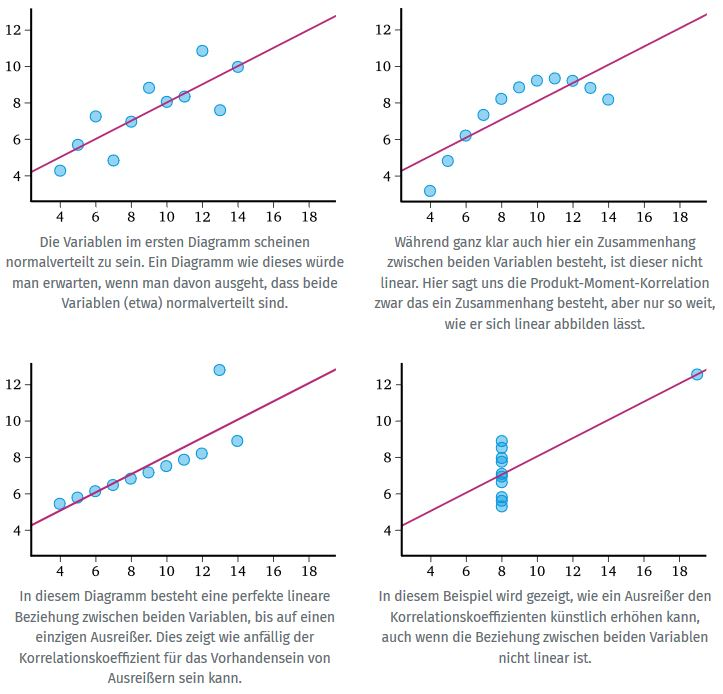
\includegraphics[width=0.80000\textwidth]{Images/03_LinearitaetKorrelation.JPG}
\caption{\textbf{Abbildung 1}: Korrelation und Linearität}
\end{figure}

\subsection*{Korrelationskoeffizienten}\label{korrelationskoeffizienten}
\addcontentsline{toc}{subsection}{Korrelationskoeffizienten}

Neben dem Pearson-Produkt-Moment-Korrelationskoeffizienten \(r\)
existieren noch etliche weitere Korrelationskoeffizienten und
Zusammenhangsmaße. Die meisten hiervon sind Sonderfälle der
Pearson-Produkt-Moment-Korrelation. Nachfolgende Tabelle zeigt, wann
welcher Koeffizient berechnet werden soll. Die Verwendung
unterschiedlicher Korrelationsberechnungen ist i.A. abhängig vom
Skalenniveau der beteiligten Variablen.

\begin{figure}
\centering
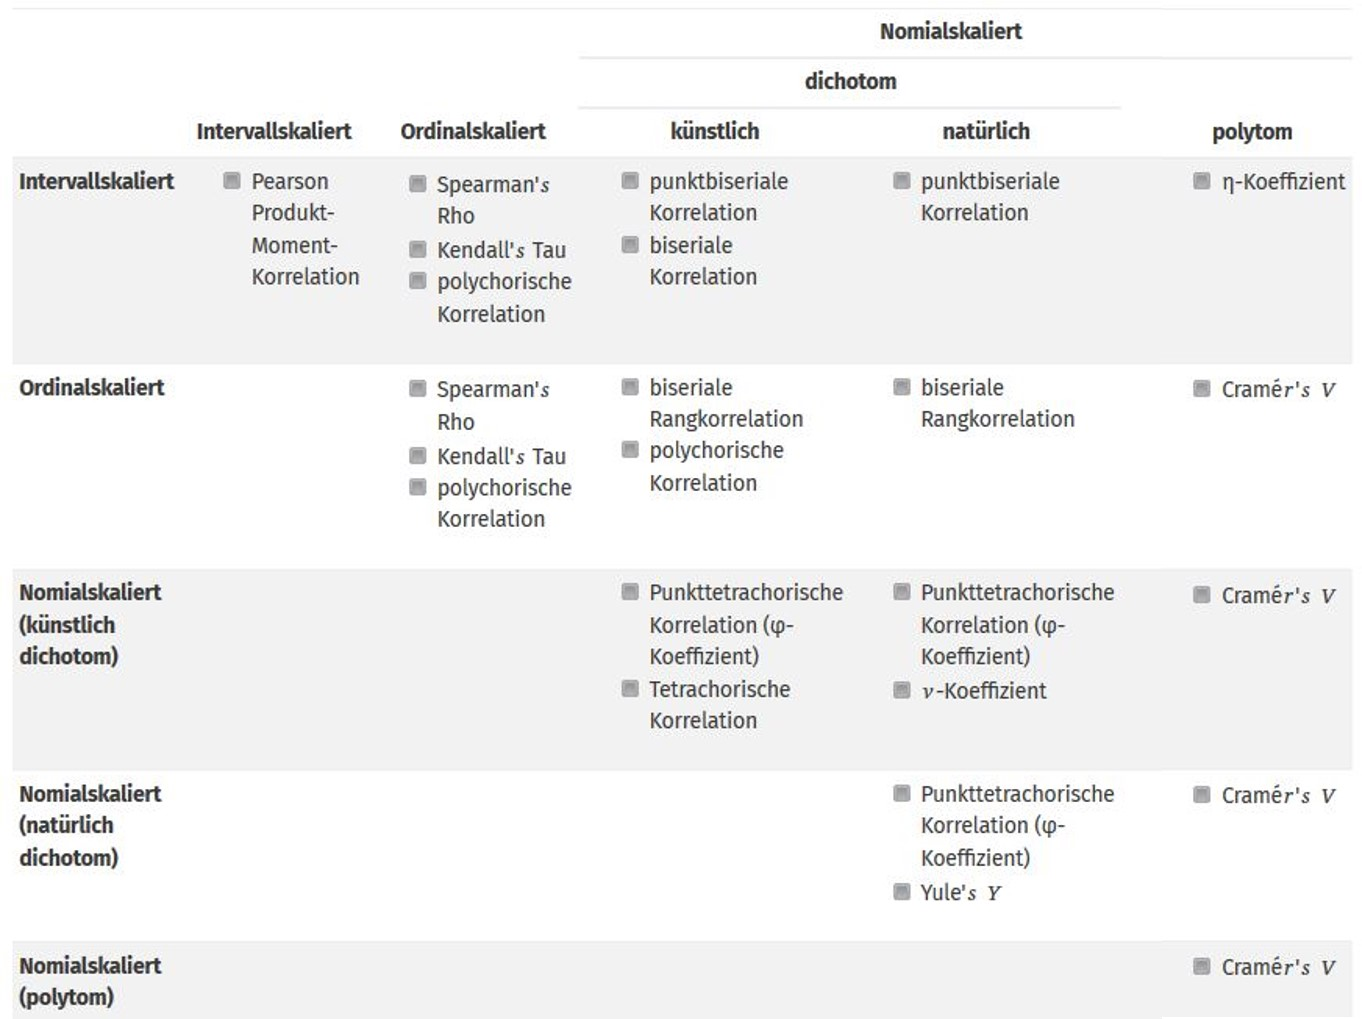
\includegraphics[width=1.00000\textwidth]{Images/Korrelationskoeffizienten.JPG}
\caption{\textbf{Abbildung 2}: verschiedene Korrelationskoeffizienten}
\end{figure}

Weiter Infos zu den einzelnen Korrelationskoeffizienten sind der
Literatur zu entnehmen. Eine übersichtliche Darstellung findet man auch
auf der Website von
\href{https://matheguru.com/stochastik/korrelation-korrelationskoeffizient.html}{MatheGuru}.

\subsection*{Herleitung}\label{herleitung}
\addcontentsline{toc}{subsection}{Herleitung}

Bereits bei der deskriptiven Statistik haben wir mit dem Maß der Varianz
(\(s^2\)) einen Kennwert definiert, der die Schwankungen bezüglich des
entsprechenden Mittelwertes beschreibt. Per Definition ist die Varianz
die durchschnittliche Summe der quadrierten Abweichungen zum Mittelwert,
also:

\begin{equation} 
  s^2 = \frac{\sum_{i=1}^{N} (x_i - \bar{x})^2}{N-1}
  \label{eq:Var}
\end{equation}

Betrachtet man zwei (normalverteilte) intervallskalierte Variablen \(x\)
und \(y\), dann lässt sich diese Idee auch als ein Kennwert der
gemeinsamen Variablität der beiden Variablen definieren:

\begin{equation} 
  cov(x,y) = \frac{\sum_{i=1}^{N} (x_i - \bar{x}) \cdot (y_i - \bar{y})}{N-1}
  \label{eq:Cov}
\end{equation}

Dieser Kennwert nennt sich \emph{Kovarianz} (\(cov\)). Da dieser
Kennwert an die entsprechenden Einheiten der Variablen gebunden ist,
normiert man i.A. dieses Maß durch das Produkt der jeweiligen
Standardabweichung \(s_x\) und \(s_y\). Dieses normierte Maß bezeichnet
man als \emph{Korrelationskoeffizient} (\(r\)):

\begin{equation} 
  r(x,y) = \frac{cov(x,y)}{s_x \cdot s_y}
  \label{eq:Korr}
\end{equation}

\subsubsection*{Beispiel}\label{beispiel}
\addcontentsline{toc}{subsubsection}{Beispiel}

Anhand des bereits verwendeten Datensatzes (\emph{CPS85}) wollen wir die
Beziehung der Variablen Gehalt (\emph{wage}), Ausbildung (\emph{educ})
und Berufserfahrung (\emph{exper}) berechnen und graphisch darstellen.
Kopiere den folgenden Code ins RStudio und führe diesen dann aus.
Diskutiere die Ergebnisse.

\begin{Shaded}
\begin{Highlighting}[]
\NormalTok{  M      <-}\StringTok{ }\KeywordTok{data.frame}\NormalTok{(}\DataTypeTok{wage =}\NormalTok{ CPS85}\OperatorTok{$}\NormalTok{wage, }\DataTypeTok{educ =}\NormalTok{ CPS85}\OperatorTok{$}\NormalTok{educ, }\DataTypeTok{exper =}\NormalTok{ CPS85}\OperatorTok{$}\NormalTok{exper)}
\NormalTok{  Korr_}\DecValTok{1}\NormalTok{ <-}\StringTok{ }\KeywordTok{cor}\NormalTok{(M)}
  \KeywordTok{pander}\NormalTok{(Korr_}\DecValTok{1}\NormalTok{, }\DataTypeTok{style =} \StringTok{"rmarkdown"}\NormalTok{)}
  \CommentTok{# DT::datatable(round(Korr_1,2))}
  \KeywordTok{corrplot}\NormalTok{(}\KeywordTok{cor}\NormalTok{(M), }\DataTypeTok{method =} \StringTok{"ellipse"}\NormalTok{)}
\end{Highlighting}
\end{Shaded}

\section*{Einfache Regression}\label{einfache-regression}
\addcontentsline{toc}{section}{Einfache Regression}

Will man bei der Korrelationsanalyse den Zusammenhang von Variablen
beschreiben, versucht man in der Regressionsanalyse eine Variable
mittels einer linearen Funktion durch eine (oder mehrere) andere
Variablen zur \emph{erklären}. Nichts desto trotz sind Korrelation und
Regression sehr eng miteinander verknüpft.

Der Begriff Regression tauchte erstmalig 1877 in einer von Sir Francis
Galton abgefassten wissenschaftlichen Studie auf. In einer späteren
Studie über die Körpergröße von Vätern und deren Söhnen wendete er den
Gedanken der Regressionsanalyse erneut an.

Er fand heraus, dass Söhne sehr großer (kleiner) Väter zwar groß
(klein), aber etwas kleiner (größer) sind als diese. Die Körpergröße
entwickelt sich somit immer wieder in Richtung des Durchschnitts zurück.
Als Engländer bezeichnete Galton diesen Prozess als
\emph{Regression}\footnote{was mit \emph{Rückschritt}, \emph{Rückkehr}
  oder \emph{rückläufige Entwicklung} übersetzt werden kann (siehe
  \href{https://link.springer.com/chapter/10.1007/978-3-8349-7071-8_5}{Deskriptive
  Statistik und moderne Datenanalyse}).}.

Zwischen der Körpergröße der Söhne und der Väter besteht somit ein
Zusammenhang, dessen Stärke mit Hilfe der Korrelation ausgedrückt werden
könnte. Im Unterschied zur Korrelationsanalyse unterstellt man bei der
Regressionsanalyse jedoch sehr oft auch die kausale Richtung des
Zusammenhangs:

\begin{quote}
Die Körpergröße der Söhne ist abhängig von der Körpergröße des Vaters
und nicht umgekehrt.
\end{quote}

Entsprechend bezeichnete Galton:

\begin{itemize}
\tightlist
\item
  die Größe der Söhne als \emph{abhängige Variable} (\emph{dependent
  variable}, \textbf{DV}) und
\item
  die Größe der Väter als \emph{unabhängige Variable} (\emph{independent
  variable}, \textbf{IV}).
\end{itemize}

Häufig werden die Variable die vorhergesagt werden soll bei der
Regression \emph{Kriterium} (\(y_i\))und die Variable(n) die für die
Vorhersage eingesetzt wird/werden \emph{Prädiktor(n)}
(\(x_{1i}\))\footnote{wobei die 1 für den ersten (einzigen) Prädiktor
  und \(i\) als Index für die \(i\)-te Beobachtung steht.} genannt.
Anhand des Prädiktors wird demzufolge das Kriterium vorhergesagt.

Der Schluss, dass die Regression die Kausalität von Zusammenhängen
\emph{beweist}, ist damit allerdings nicht (immer) erlaubt. Die
Kausalität (Wirkungsrichtung) muss zuvor theoretisch abgeleitet werden,
bevor sie empirisch (mit Hilfe der Regression) bewiesen werden kann. So
ist die Richtung der Kausalität bei Fragen wie:

\begin{itemize}
\tightlist
\item
  ist es das Alter des Bräutigams, welches das Alter der Braut bestimmt,
  oder umgekehrt?
\item
  beeinflusst sich das Alter der verheirateten Paare gar gegenseitig?
\end{itemize}

nicht zu bestimmen. Manchmal ist die Kausalität jedoch sehr
offensichtlich:

\begin{itemize}
\tightlist
\item
  der Blutdruck hat keinen Einfluss auf das Alter, sondern das Alter hat
  einen Einfluss auf den Blutdruck.
\item
  die Körpergröße hat einen Einfluss auf das Körpergewicht, aber
  umgekehrt lässt sich dieser Zusammenhang wohl theoretisch kaum
  herleiten.
\item
  mit Zunahme des \(CO_2\) Gehaltes in der Atmosphäre steigt die
  durchschnittliche Temperatur, eine umgekehrte Wirkungsrichtung ist
  aber auszuschließen (da hätten wir in südlichen Ländern ein kleines
  Problem!).
\end{itemize}

Die Regression ermöglicht jedenfalls unter bestimmten
Umständen\footnote{intervallskaliertes Kriterium, linearer Zusammenhang
  zw. Kriterium und Prädiktor(en), Zufallsstichprobe, Normalverteilung
  der Fehler, Homoskedastizität, Unabhängigkeit der Fehler. Details dazu
  später.} gute, bzw. bestmögliche Vorhersage für eine Variable.
Folgernd aus dem eben gesagten, sollte nochmals klargestellt werden,
dass im Gegensatz zur Korrelation festgelegt werden muss, welche
Variable durch eine andere Variable vorhergesagt werden soll.

\subsection*{Definitionen}\label{definitionen}
\addcontentsline{toc}{subsection}{Definitionen}

Die formale Definition eines einfachen linearen Modells ist:

\begin{equation} 
  y_i = b_0 + b_1 \cdot x_{1i} + \varepsilon_i
  \label{eq:LinModFehler}
\end{equation}

Die wesentlichen Parameter dieses einfachen Modells sind:

\begin{enumerate}
\def\labelenumi{\arabic{enumi}.}
\tightlist
\item
  Konstanter Term (intercept) \(b_0\): jener Wert den \(y_i\) einnimmt,
  wenn \(x_{1i} = 0\) ist.
\item
  Steigung (slope) \(b_1\): die Zunahme von \(y_i\), wenn \(x_{1i}\)
  sich um eine Einheit erhöht.
\end{enumerate}

Des Weiteren berücksichtigt dieses Modell auch einen Fehler
(\(\varepsilon_i\)). Damit kommt auch ein ganz zentraler Teil bei der
Modellbildung zum Ausdruck. Die meisten Modelle definieren sich also
aus:

\begin{equation} 
  \textrm{wahrer Wert} = \textrm{Modell} + \textrm{Fehler}
  \label{eq:AllgModellvorstellung}
\end{equation}

Daraus lässt sich auch folgende Erkenntnis bezüglich des Modells direkt
ableiten:

\begin{enumerate}
\def\labelenumi{\arabic{enumi}.}
\tightlist
\item
  Je kleiner die Summe der Fehler sind, desto besser ist das Modell.
\item
  Je genauer das Modell, desto kleiner wird auch der Fehler sein.
\end{enumerate}

Mit dieser Erkenntnis wird auch klar, dass i.A. ein ganz einfaches
Modell (mit einem einzigen Prädiktor) nur zu einer bedingten Reduktion
des Fehlers geeignet ist. Wir werden uns im weiteren Verlauf mit
erweiterten Modellen beschäftigen, wollen aber zunächst die
Eigenschaften des einfachen linearen Modells näher betrachten. Im
folgenden Link findet man eine gute
\href{https://phet.colorado.edu/sims/html/least-squares-regression/latest/least-squares-regression_en.html}{Veranschaulichung
des einfachen linearen Modells}.

Betrachtet man das Modell isoliert (also ohne Fehlerterm), ist folgende
Schreibweise üblich:

\begin{equation} 
  \hat{y}_i = b_0 + b_1 \cdot x_{1i}
  \label{eq:LinMod}
\end{equation}

\subsubsection*{Berechnung der
Koeffizienten}\label{berechnung-der-koeffizienten}
\addcontentsline{toc}{subsubsection}{Berechnung der Koeffizienten}

Für die Berechnung der Koeffizienten wird das Kriterium der kleinste
Quadrate (MLS) angewandet. Einfach ausgedrückt wird eine Gerade durch
die beobachteten Daten gesucht, die folgenden Eigenschaften aufweist:

\begin{enumerate}
\def\labelenumi{\arabic{enumi}.}
\tightlist
\item
  die Summe der quadratischen Abstände jeder Beobachtung zum
  entsprechenden Punkt auf der Geraden ist ein Minimum, also
  \(\sum_{i=1}^{N} \varepsilon_i^2 = min\).
\item
  es gibt keine andere Gerade die eine kleinere Summe dieser Fehler
  liefert.
\end{enumerate}

Die Berechnung der Parameter entspricht daher einer Extremwertaufgabe,
d.h. die partiellen Ableitungen werden auf Null gesetzt. Daraus lassen
sich dann die Parameter \(b_0, b_1\) berechnent. Details dazu siehe
\href{https://de.wikipedia.org/wiki/Einfache_lineare_Regression}{Wikipedia}.

\subsection*{Modellanwendung}\label{modellanwendung}
\addcontentsline{toc}{subsection}{Modellanwendung}

Zur Anwendung eines einfachen linearen Modell betrachten wir wiederum
die bereits bekannten Daten aus dem Datensatz \emph{CPS85}. Diese Mal
wollen wir das Gehalt (\emph{wage}) durch die Ausbildungsdauer
(\emph{educ} in Jahren) vorhersagen. Formal lautet das Modell demnach:

\begin{equation} 
   \hat{\textrm{wage}} = b_0 + b_1 \cdot \textrm{educ}
  \label{eq:LinModBsp1}
\end{equation}

Die Werte der Parameter \(b_0, b_1\) können für dieses Beispiel
entsprechend der obigen Erläuterung folgendermaßen interpretiert werden:

\begin{enumerate}
\def\labelenumi{\arabic{enumi}.}
\tightlist
\item
  Für eine Person mit keiner Ausbildung (\(\textrm{wage} = x_{1i} = 0\))
  wird durch das Modell ein Einkommen \(y_i = b_0\) vorhergesagt.
\item
  Erhöht man die Ausbildungsdauer \(x_{1i}\) um ein Jahr, steigt der
  Gehalt \(y_i\) um das \(b_1\)-fache an.
\end{enumerate}

Kopiere zur Veranschaulichung folgenden Code in dein R-Script und führe
diesen aus.

\begin{Shaded}
\begin{Highlighting}[]
\NormalTok{  DF <-}\StringTok{ }\NormalTok{CPS85}
  \KeywordTok{ggplot}\NormalTok{(CPS85, }\KeywordTok{aes}\NormalTok{(}\DataTypeTok{x =}\NormalTok{ educ, }\DataTypeTok{y =}\NormalTok{ wage)) }\OperatorTok{+}
\StringTok{    }\KeywordTok{geom_point}\NormalTok{() }\OperatorTok{+}
\StringTok{    }\KeywordTok{geom_smooth}\NormalTok{(}\DataTypeTok{method=}\NormalTok{lm, }\DataTypeTok{se=}\OtherTok{FALSE}\NormalTok{) }\OperatorTok{+}
\StringTok{    }\KeywordTok{theme_bw}\NormalTok{()}
\end{Highlighting}
\end{Shaded}

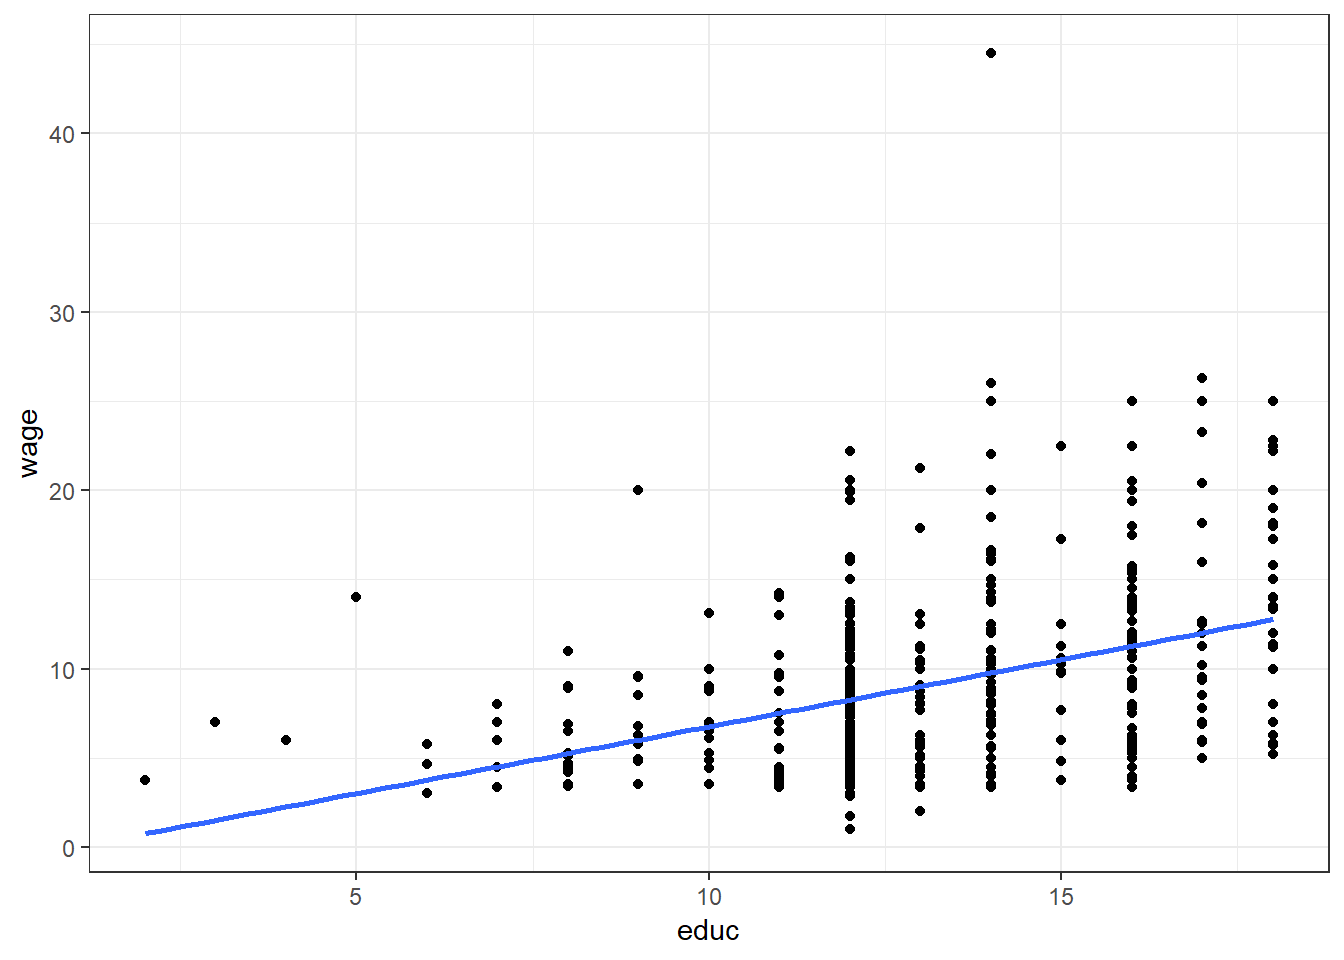
\includegraphics{03_Modelle_Mehr_Variablen_files/figure-latex/Modell1-1.pdf}

\begin{Shaded}
\begin{Highlighting}[]
\NormalTok{  model_}\DecValTok{1}\NormalTok{     <-}\StringTok{ }\KeywordTok{lm}\NormalTok{(wage }\OperatorTok{~}\StringTok{ }\NormalTok{educ, }\DataTypeTok{data =}\NormalTok{ CPS85)}
  \KeywordTok{pander}\NormalTok{(}\KeywordTok{summary}\NormalTok{(model_}\DecValTok{1}\NormalTok{))}
\end{Highlighting}
\end{Shaded}

\begin{longtable}[]{@{}ccccc@{}}
\toprule
\begin{minipage}[b]{0.21\columnwidth}\centering\strut
~\strut
\end{minipage} & \begin{minipage}[b]{0.13\columnwidth}\centering\strut
Estimate\strut
\end{minipage} & \begin{minipage}[b]{0.16\columnwidth}\centering\strut
Std. Error\strut
\end{minipage} & \begin{minipage}[b]{0.12\columnwidth}\centering\strut
t value\strut
\end{minipage} & \begin{minipage}[b]{0.13\columnwidth}\centering\strut
Pr(\textgreater{}\textbar{}t\textbar{})\strut
\end{minipage}\tabularnewline
\midrule
\endhead
\begin{minipage}[t]{0.21\columnwidth}\centering\strut
\textbf{(Intercept)}\strut
\end{minipage} & \begin{minipage}[t]{0.13\columnwidth}\centering\strut
-0.746\strut
\end{minipage} & \begin{minipage}[t]{0.16\columnwidth}\centering\strut
1.045\strut
\end{minipage} & \begin{minipage}[t]{0.12\columnwidth}\centering\strut
-0.7135\strut
\end{minipage} & \begin{minipage}[t]{0.13\columnwidth}\centering\strut
0.4758\strut
\end{minipage}\tabularnewline
\begin{minipage}[t]{0.21\columnwidth}\centering\strut
\textbf{educ}\strut
\end{minipage} & \begin{minipage}[t]{0.13\columnwidth}\centering\strut
0.7505\strut
\end{minipage} & \begin{minipage}[t]{0.16\columnwidth}\centering\strut
0.07873\strut
\end{minipage} & \begin{minipage}[t]{0.12\columnwidth}\centering\strut
9.532\strut
\end{minipage} & \begin{minipage}[t]{0.13\columnwidth}\centering\strut
5.474e-20\strut
\end{minipage}\tabularnewline
\bottomrule
\end{longtable}

\begin{longtable}[]{@{}cccc@{}}
\caption{Fitting linear model: wage \textasciitilde{}
educ}\tabularnewline
\toprule
\begin{minipage}[b]{0.18\columnwidth}\centering\strut
Observations\strut
\end{minipage} & \begin{minipage}[b]{0.27\columnwidth}\centering\strut
Residual Std. Error\strut
\end{minipage} & \begin{minipage}[b]{0.11\columnwidth}\centering\strut
\(R^2\)\strut
\end{minipage} & \begin{minipage}[b]{0.20\columnwidth}\centering\strut
Adjusted \(R^2\)\strut
\end{minipage}\tabularnewline
\midrule
\endfirsthead
\toprule
\begin{minipage}[b]{0.18\columnwidth}\centering\strut
Observations\strut
\end{minipage} & \begin{minipage}[b]{0.27\columnwidth}\centering\strut
Residual Std. Error\strut
\end{minipage} & \begin{minipage}[b]{0.11\columnwidth}\centering\strut
\(R^2\)\strut
\end{minipage} & \begin{minipage}[b]{0.20\columnwidth}\centering\strut
Adjusted \(R^2\)\strut
\end{minipage}\tabularnewline
\midrule
\endhead
\begin{minipage}[t]{0.18\columnwidth}\centering\strut
534\strut
\end{minipage} & \begin{minipage}[t]{0.27\columnwidth}\centering\strut
4.754\strut
\end{minipage} & \begin{minipage}[t]{0.11\columnwidth}\centering\strut
0.1459\strut
\end{minipage} & \begin{minipage}[t]{0.20\columnwidth}\centering\strut
0.1443\strut
\end{minipage}\tabularnewline
\bottomrule
\end{longtable}

Die in der Tabelle angegebenen Werte der Spalte \textbf{Estimate}
entsprechen dabei den Parametern \(b_0, b_1\) des Modells. Eine weitere
wesentliche Kennzahl für die Interpretation des Modells ist der Spalte
\(R^2\) zu entnehmen. Dieser Wert wird als
\emph{Determinationskoeffizient}\footnote{häufig auch als
  Varianzaufklärung} bezeichnet. Umgerechnet in \% (im vorliegenden
Beispiel also 14.43\%) besagt der Wert, wie viel der Variablität des
Gehaltes durch den Prädiktor Ausbilung erklärt wird. Wir werden im
weiteren Verlauf noch öfter auf diesen Kennwert zurückkommen.

Welche Gehälter würden für Ausbildungszeiten zwischen 10 und 14 Jahren
vorhergesagt werden? Kopiere folgenden Code in dein R-Script und führe
diesen aus. Änder auch den Wertebereich der Prädiktoren und beobachte
was dabei passiert!

Im Vergleich zum Mittelwert-Modell zeigt sich mit steigender Ausbildung
ein höheres Einkommen. Der Fehler bei der Vorhersage des Einkommens wird
sich daher durch diese Modellvorstellung verringern (mehr zur
Abschätzung der Fehlerreduktion später).

\hypertarget{aufgabe-slr-1}{\subsubsection*{Aufgabe SLR
1}\label{aufgabe-slr-1}}
\addcontentsline{toc}{subsubsection}{Aufgabe SLR 1}

Öffne ein neues R-Script und kopiere die bereits bekannte Kopfzeile in
diese Datei. Speichere anschließend das Skript unter dem Namen
\emph{SLR\_Aufgabe1.R}. Bearbeite nun folgende Aufgabenstellungen:

\begin{itemize}
\tightlist
\item
  Lade die Datei ``\emph{Album Sales 1.dat}''
\item
  erstelle ein einfaches Streudiagramm mit Sales auf der x- und adverts
  auf der y-Achse.
\item
  erstelle ein einfaches lineares Modell zur Vorhersage der
  Verkaufszahlen (\emph{sales}) durch die Variable \emph{adverts}.
\item
  Wie stark korrelliert der Prädiktor mit dem Kriterium?
\item
  Wie viel Varianz wird vom Kriterium durch den Prädiktor aufgeklärt?
\item
  Ist das erstellte Modell signifikant besser, als dan Null-Modell?
\item
  Welchen Wert würde das Modell für Werbeausgaben = 100 vorhersagen?
\end{itemize}

\protect\hyperlink{aufgabe-slr-1-lsg}{Lösung Aufgabe SLR 1}

\subsection*{Residualanalyse}\label{residualanalyse}
\addcontentsline{toc}{subsection}{Residualanalyse}

Ein zentrales Thema der Modellbildung ist die Beurteilung und
(statistische) Auswertung der Abweichungen des Modells von den
Beobachtungen (Fehler, Residum). Folgende Kennwerte bilden die
Möglichkeit, die Güte des Modells abzuschätzen:

\begin{enumerate}
\def\labelenumi{\arabic{enumi}.}
\tightlist
\item
  \emph{Vorhergesagte Werte}: vorhergesagte Werte der
  Regressionsgleichung (= Werte die auf der Geraden liegen).

  \begin{itemize}
  \tightlist
  \item
    Nicht standardisiert: der Wert, den das Modell für die abhängige
    Variable vorhersagt.
  \item
    Standardisiert: \(z\)-Transformierte vorhergesagte Werte.
  \item
    Korrigiert: der vorhergesagte Wert für einen Fall, wenn dieser Fall
    von der Berechnung der Regressionskoeffizienten ausgeschlossen ist.
  \item
    Standardfehler des Mittelwerts: Standardfehler der vorhergesagten
    Werte. Ein Schätzwert der Standardabweichung des Durchschnittswertes
    der abhängigen Variablen für die Fälle, die dieselben Werte für die
    unabhängigen Variablen haben.
  \end{itemize}
\item
  \emph{Residuen}: tatsächliche Wert der abhängigen Variablen minus des
  vorhergesagten Werts aus der Regressionsgleichung.

  \begin{itemize}
  \tightlist
  \item
    Nicht standardisiert: Die Differenz zwischen einem beobachteten Wert
    und dem durch das Modell vorhergesagten Wert.
  \item
    Standardisiert: Der Quotient aus dem Residuum und einer Schätzung
    seiner Standardabweichung. Standardisierte Residuen, auch bekannt
    als Pearson-Residuen, haben einen Mittelwert von 0 und eine
    Standardabweichung von 1.
  \item
    Studentisiert: Ein Residuum, das durch seine geschätzte
    Standardabweichung geteilt wird, die je nach der Distanz zwischen
    den Werten der unabhängigen Variablen des Falles und dem Mittelwert
    der unabhängigen Variablen von Fall zu Fall variiert.
  \item
    Ausgeschlossen: Das Residuum für einen Fall, wenn dieser Fall nicht
    in die Berechnung der Regressionskoeffizienten eingegangen ist. Dies
    ist die Differenz zwischen dem Wert der abhängigen Variablen und dem
    korrigierten Schätzwert.
  \item
    Studentisiert und ausgeschlossen: Der Quotient aus dem
    ausgeschlossenen Residuum eines Falles und seinem Standardfehler.
    Die Differenz zwischen einem studentisierten ausgeschlossenen
    Residuum und dem zugehörigen studentisierten Residuum gibt an,
    welchen Unterschied die Entfernung eines Falles für dessen eigene
    Vorhersage bewirkt.
  \end{itemize}
\item
  \emph{Distanzen}: Maße zum Auffinden von Fällen mit ungewöhnlichen
  Wertekombinationen bei den unabhängigen Variablen und von Fällen, die
  einen großen Einfluss auf das Modell haben könnten.

  \begin{itemize}
  \tightlist
  \item
    Mahalanobis: Dieses Maß gibt an, wie weit die Werte der unabhängigen
    Variablen eines Falls vom Mittelwert aller Fälle abweichen. Eine
    große Mahalanobis-Distanz charakterisiert einen Fall, der bei einer
    oder mehreren unabhängigen Variablen Extremwerte besitzt.
  \item
    Cook: Ein Maß dafür, wie stark sich die Residuen aller Fälle ändern
    würden, wenn ein spezieller Fall von der Berechnung der
    Regressionskoeffizienten ausgeschlossen würde. Ein großer Wert der
    Cook-Distanz zeigt an, dass der Ausschluss eines Falles von der
    Berechnung der Regressionskoeffizienten die Koeffizienten
    substanziell verändert.
  \item
    Hebelwerte: Werte, die den Einfluss eines Punktes auf die Anpassung
    der Regression messen. Der zentrierte Wert für die Hebelwirkung
    bewegt sich zwischen 0 (kein Einfluss auf die Anpassung) und
    \((N-1)/N\).
  \end{itemize}
\item
  \emph{Vorhersageintervalle}: obere und untere Grenzen sowohl für
  Mittelwert als auch für einzelne Vorhersageintervalle.

  \begin{itemize}
  \tightlist
  \item
    Mittelwert: Unter- und Obergrenze (zwei Variablen) für das
    Vorhersageintervall für den mittleren vorhergesagten Wert.
  \item
    Individuell: Unter- und Obergrenzen (zwei Variablen) für das
    Vorhersageintervall der abhängigen Variablen für einen Einzelfall.
  \item
    Konfidenzintervall: Geben Sie einen Wert zwischen 1 und 99,99 ein,
    um das Konfidenzniveau für die beiden Vorhersageintervalle
    festzulegen. Wählen Sie \emph{Mittelwert} oder \emph{Individuell}
    aus, bevor Sie diesen Wert eingeben. Typische Werte für
    Konfidenzniveaus sind 90, 95 und 99.
  \end{itemize}
\item
  \emph{Einflussstatistiken}: Änderung in den Regressionskoeffizienten
  (DfBeta(s)) und vorhergesagten Werten (DfFit), die sich aus dem
  Ausschluss eines bestimmten Falls ergeben.

  \begin{itemize}
  \tightlist
  \item
    Differenz in Beta: entspricht der Änderung im
    Regressionskoeffizienten, die sich aus dem Ausschluss eines
    bestimmten Falls ergibt. Für jeden Term im Modell, einschließlich
    der Konstanten, wird ein Wert berechnet.
  \item
    Standardisiertes DfBeta: die Änderung des Regressionskoeffizienten,
    die sich durch den Ausschluss eines bestimmten Falls ergibt. Es
    empfiehlt sich, Fälle mit absoluten Werten größer als \(2/\sqrt{N}\)
    zu überprüfen, wenn \(N\) die Anzahl der Fälle darstellt. Für jeden
    Term im Modell, einschließlich der Konstanten, wird ein Wert
    berechnet.
  \item
    DfFit: Differenz im Anpassungswert ist die Änderung im
    vorhergesagten Wert, die sich aus dem Ausschluss eines bestimmten
    Falls ergibt.
  \item
    Standardisiertes DfFit: Änderung des vorhergesagten Werts, die sich
    durch den Ausschluss eines bestimmten Falls ergibt. Es empfiehlt
    sich, Fälle mit absoluten Werten \(> 2/\sqrt{p/N}\) zu überprüfen,
    wobei \(p\) die Anzahl der unabhängigen Variablen im Modell und
    \(N\) die Anzahl der Fälle darstellt.
  \item
    Kovarianzverhältnis: Verhältnis der Determinante der Kovarianzmatrix
    bei Ausschluss eines bestimmten Falls von der Berechnung der
    Regressionskoeffizienten zur Determinante der Kovarianzmatrix bei
    Einschluss aller Fälle. Wenn der Quotient dicht bei 1 liegt,
    beeinflusst der ausgeschlossene Fall die Kovarianzmatrix nur
    unwesentlich.
  \end{itemize}
\end{enumerate}

Nachfolgender Code und Tabelle zeigen die Auswertung der Residualanalyse
für das oben erstellte \emph{model\_1}:

\begin{Shaded}
\begin{Highlighting}[]
\NormalTok{  CPS85_Res <-}\StringTok{ }\KeywordTok{data.frame}\NormalTok{(}\DataTypeTok{Res     =} \KeywordTok{round}\NormalTok{(}\KeywordTok{resid}\NormalTok{(model_}\DecValTok{1}\NormalTok{), }\DecValTok{2}\NormalTok{),}
                          \DataTypeTok{StdRes  =} \KeywordTok{round}\NormalTok{(}\KeywordTok{rstandard}\NormalTok{(model_}\DecValTok{1}\NormalTok{), }\DecValTok{2}\NormalTok{),}
                          \DataTypeTok{StudRes =} \KeywordTok{round}\NormalTok{(}\KeywordTok{rstudent}\NormalTok{(model_}\DecValTok{1}\NormalTok{), }\DecValTok{2}\NormalTok{),}
                          \CommentTok{# Cook    = round(cooks.distance(model_1), 2),}
                          \CommentTok{# DFBeta  = round(dfbeta(model_1), 2),}
                          \DataTypeTok{DF5Fit  =} \KeywordTok{round}\NormalTok{(}\KeywordTok{dffits}\NormalTok{(model_}\DecValTok{1}\NormalTok{), }\DecValTok{2}\NormalTok{),}
                          \CommentTok{# Lev     = round(hatvalues(model_1), 2),}
                          \DataTypeTok{CovRat  =} \KeywordTok{round}\NormalTok{(}\KeywordTok{covratio}\NormalTok{(model_}\DecValTok{1}\NormalTok{), }\DecValTok{2}\NormalTok{))}
  \KeywordTok{pander}\NormalTok{(}\KeywordTok{head}\NormalTok{(CPS85_Res))}
\end{Highlighting}
\end{Shaded}

\begin{longtable}[]{@{}ccccc@{}}
\toprule
\begin{minipage}[b]{0.10\columnwidth}\centering\strut
Res\strut
\end{minipage} & \begin{minipage}[b]{0.11\columnwidth}\centering\strut
StdRes\strut
\end{minipage} & \begin{minipage}[b]{0.12\columnwidth}\centering\strut
StudRes\strut
\end{minipage} & \begin{minipage}[b]{0.11\columnwidth}\centering\strut
DF5Fit\strut
\end{minipage} & \begin{minipage}[b]{0.11\columnwidth}\centering\strut
CovRat\strut
\end{minipage}\tabularnewline
\midrule
\endhead
\begin{minipage}[t]{0.10\columnwidth}\centering\strut
2.24\strut
\end{minipage} & \begin{minipage}[t]{0.11\columnwidth}\centering\strut
0.47\strut
\end{minipage} & \begin{minipage}[t]{0.12\columnwidth}\centering\strut
0.47\strut
\end{minipage} & \begin{minipage}[t]{0.11\columnwidth}\centering\strut
0.03\strut
\end{minipage} & \begin{minipage}[t]{0.11\columnwidth}\centering\strut
1.01\strut
\end{minipage}\tabularnewline
\begin{minipage}[t]{0.10\columnwidth}\centering\strut
-2.76\strut
\end{minipage} & \begin{minipage}[t]{0.11\columnwidth}\centering\strut
-0.58\strut
\end{minipage} & \begin{minipage}[t]{0.12\columnwidth}\centering\strut
-0.58\strut
\end{minipage} & \begin{minipage}[t]{0.11\columnwidth}\centering\strut
-0.03\strut
\end{minipage} & \begin{minipage}[t]{0.11\columnwidth}\centering\strut
1\strut
\end{minipage}\tabularnewline
\begin{minipage}[t]{0.10\columnwidth}\centering\strut
-4.46\strut
\end{minipage} & \begin{minipage}[t]{0.11\columnwidth}\centering\strut
-0.94\strut
\end{minipage} & \begin{minipage}[t]{0.12\columnwidth}\centering\strut
-0.94\strut
\end{minipage} & \begin{minipage}[t]{0.11\columnwidth}\centering\strut
-0.04\strut
\end{minipage} & \begin{minipage}[t]{0.11\columnwidth}\centering\strut
1\strut
\end{minipage}\tabularnewline
\begin{minipage}[t]{0.10\columnwidth}\centering\strut
2.24\strut
\end{minipage} & \begin{minipage}[t]{0.11\columnwidth}\centering\strut
0.47\strut
\end{minipage} & \begin{minipage}[t]{0.12\columnwidth}\centering\strut
0.47\strut
\end{minipage} & \begin{minipage}[t]{0.11\columnwidth}\centering\strut
0.02\strut
\end{minipage} & \begin{minipage}[t]{0.11\columnwidth}\centering\strut
1.01\strut
\end{minipage}\tabularnewline
\begin{minipage}[t]{0.10\columnwidth}\centering\strut
6.74\strut
\end{minipage} & \begin{minipage}[t]{0.11\columnwidth}\centering\strut
1.42\strut
\end{minipage} & \begin{minipage}[t]{0.12\columnwidth}\centering\strut
1.42\strut
\end{minipage} & \begin{minipage}[t]{0.11\columnwidth}\centering\strut
0.07\strut
\end{minipage} & \begin{minipage}[t]{0.11\columnwidth}\centering\strut
1\strut
\end{minipage}\tabularnewline
\begin{minipage}[t]{0.10\columnwidth}\centering\strut
-2.26\strut
\end{minipage} & \begin{minipage}[t]{0.11\columnwidth}\centering\strut
-0.48\strut
\end{minipage} & \begin{minipage}[t]{0.12\columnwidth}\centering\strut
-0.48\strut
\end{minipage} & \begin{minipage}[t]{0.11\columnwidth}\centering\strut
-0.03\strut
\end{minipage} & \begin{minipage}[t]{0.11\columnwidth}\centering\strut
1.01\strut
\end{minipage}\tabularnewline
\bottomrule
\end{longtable}

Mit der Residualanalyse kann man auf relativ einfache Weise jene Werte
ermitteln (und auch graphisch darstellen), die z.B. um mehr als eine
Standardabweichung abweichen. Diese Werte könnte man nochmals genauer
untersuchen und gegebenenfalls vor einer weiterführenden Analyse
ausschließen\footnote{der Ausschluss von Werten ist nur dann erlaubt,
  wenn eine entsprechende Begründung (nachvollziehbarer Messfehler,
  falsche Datenübertragung, etc.) vorliegt!}. Keinesfalls sollte sie
jedoch dazu verwendet werden, um einen erwünschten Effekt durch
schrittweises löschen störender Daten zu erreichen! Kopiere folgenden
Code in dein R-Script und führe diesen aus.

\begin{Shaded}
\begin{Highlighting}[]
  \CommentTok{# Liste standardisierte Residuen > |1|}
\NormalTok{  Ind_Res <-}\StringTok{ }\KeywordTok{which}\NormalTok{((CPS85_Res}\OperatorTok{$}\NormalTok{StdRes }\OperatorTok{>}\StringTok{ }\DecValTok{1} \OperatorTok{|}\StringTok{ }\NormalTok{CPS85_Res}\OperatorTok{$}\NormalTok{StdRes }\OperatorTok{<}\StringTok{ }\OperatorTok{-}\DecValTok{1}\NormalTok{) }\OperatorTok{==}\StringTok{ }\OtherTok{TRUE}\NormalTok{)}
  \CommentTok{# Anzeige der Werte von wage und educ sowie der Standardisierten Residuen}
  \CommentTok{# für jene Fälle, deren Residuen über 1 SD abweichen.}
  
  \CommentTok{# pander(data.frame(Indizes = Ind_Res,}
  \CommentTok{#                   wage = CPS85$wage[Ind_Res],}
  \CommentTok{#                   educ = CPS85$educ[Ind_Res] ,}
  \CommentTok{#                   CPS85_Res$StdRes[Ind_Res]))}
  
\NormalTok{  p_Res1 <-}\StringTok{ }\KeywordTok{ggplot}\NormalTok{(CPS85, }\KeywordTok{aes}\NormalTok{(}\DataTypeTok{x =}\NormalTok{ educ, }\DataTypeTok{y =}\NormalTok{ wage)) }\OperatorTok{+}\StringTok{ }
\StringTok{            }\KeywordTok{geom_point}\NormalTok{() }\OperatorTok{+}
\StringTok{            }\KeywordTok{geom_point}\NormalTok{(}\DataTypeTok{data=}\NormalTok{CPS85[Ind_Res,],}\DataTypeTok{colour=}\StringTok{"red"}\NormalTok{,}\DataTypeTok{size=}\DecValTok{3}\NormalTok{) }\OperatorTok{+}
\StringTok{            }\KeywordTok{theme_bw}\NormalTok{()}
  \KeywordTok{print}\NormalTok{(p_Res1, }\DataTypeTok{comment =} \OtherTok{FALSE}\NormalTok{)}
\end{Highlighting}
\end{Shaded}

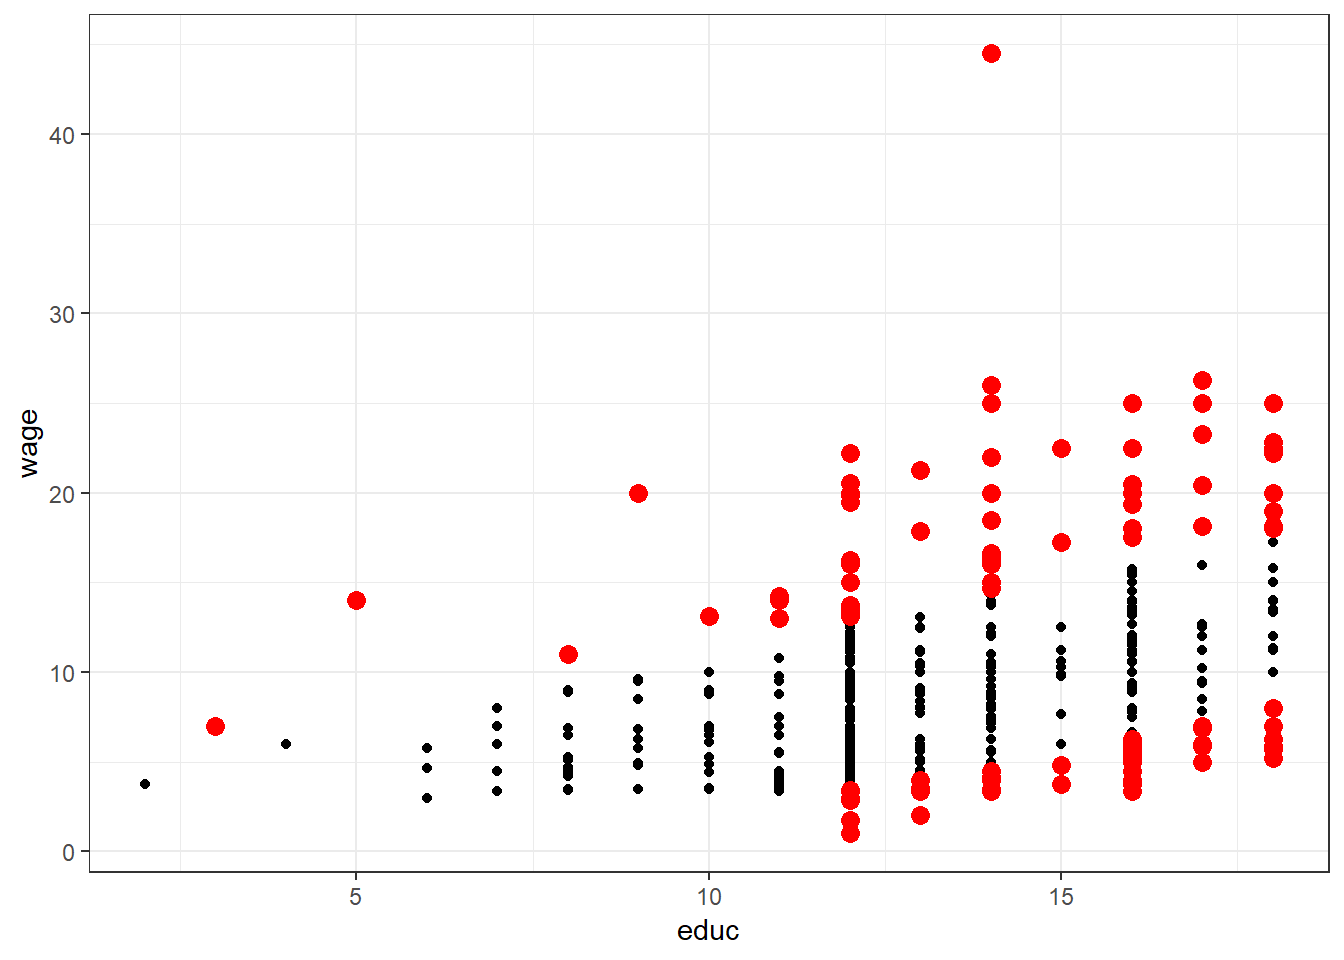
\includegraphics{03_Modelle_Mehr_Variablen_files/figure-latex/Modell1_ResidStat_Graph1-1.pdf}

\section*{Multiple Regression}\label{multiple-regression}
\addcontentsline{toc}{section}{Multiple Regression}

Man könnte nun die bereits erwähnte Variable Erfahrung (\emph{exper})
ins Modell aufnehmen. Der bereits aus der Korrelation ersichtliche
(negative) Zusammenhang mit der Ausbildung \emph{educ} lässt den Schluss
auf eine Kovariabilität der beiden Variablen zu. Man nennt derartige
Variablen auch \textbf{Kovariate}. Im linearen Modell wird diese jedoch
wie eine weitere Variable (ein weiterer Prädiktor) zur Vorhersage des
Kriteriums verwendet.

\subsection*{Definition}\label{definition}
\addcontentsline{toc}{subsection}{Definition}

Die formale Definition eines multiplen linearen Modells ist:

\begin{equation} 
  y_i = b_0 + b_1 \cdot x_{1i} + \cdots + b_k \cdot x_{ki} + \varepsilon_i
  \label{eq:LinModMultFehler}
\end{equation}

Die wesentlichen Parameter dieses Modells sind:

\begin{enumerate}
\def\labelenumi{\arabic{enumi}.}
\tightlist
\item
  Intercept \(b_0\): jener Wert den \(y_i\) einnimmt, wenn
  \(x_{ji} = 0\) ist (mit \(j \epsilon [1,k]\)).
\item
  Steigung \(b_i\): die Zunahme von \(y_i\), wenn \(x_{ji}\) sich um
  eine Einheit erhöht, bei gleichzeitigem Konstanthalten der restlichen
  Prädiktorwerte \(x_{mi}\) (mit \(m [1,k]\) und \(m \ne j\))!
\end{enumerate}

Des Weiteren berücksichtigt auch dieses Modell wieder einen Fehler
(\(\varepsilon_i\)). Betrachtet man das multiple Modell isoliert (also
ohne Fehlerterm), ist folgende Schreibweise üblich:

\begin{equation} 
  \hat{y}_i = b_0 + b_1 \cdot x_{1i} + \cdots + b_k \cdot x_{ki}
  \label{eq:LinModMult}
\end{equation}

Betrachten wir an unseren Beispieldaten folgendes Modell mit zwei
Prädiktoren:

\begin{eqnarray*} 
  \hat{wage}_i = b_0 + b_1 \cdot educ_{i} + b_2 \cdot exper_{i}
  \label{eq:LinModMultBsp}
\end{eqnarray*}

\begin{Shaded}
\begin{Highlighting}[]
\NormalTok{  model_}\DecValTok{2}\NormalTok{     <-}\StringTok{ }\KeywordTok{lm}\NormalTok{(wage }\OperatorTok{~}\StringTok{ }\NormalTok{educ }\OperatorTok{+}\StringTok{ }\NormalTok{exper, }\DataTypeTok{data =}\NormalTok{ CPS85)}
\NormalTok{  Det_model_}\DecValTok{2}\NormalTok{ <-}\StringTok{ }\KeywordTok{pander}\NormalTok{(}\KeywordTok{summary}\NormalTok{(model_}\DecValTok{2}\NormalTok{))}
  \KeywordTok{plotPlane}\NormalTok{(}\DataTypeTok{model =}\NormalTok{ model_}\DecValTok{2}\NormalTok{, }\DataTypeTok{plotx1 =} \StringTok{"educ"}\NormalTok{, }\DataTypeTok{plotx2 =} \StringTok{"exper"}\NormalTok{)}
\end{Highlighting}
\end{Shaded}

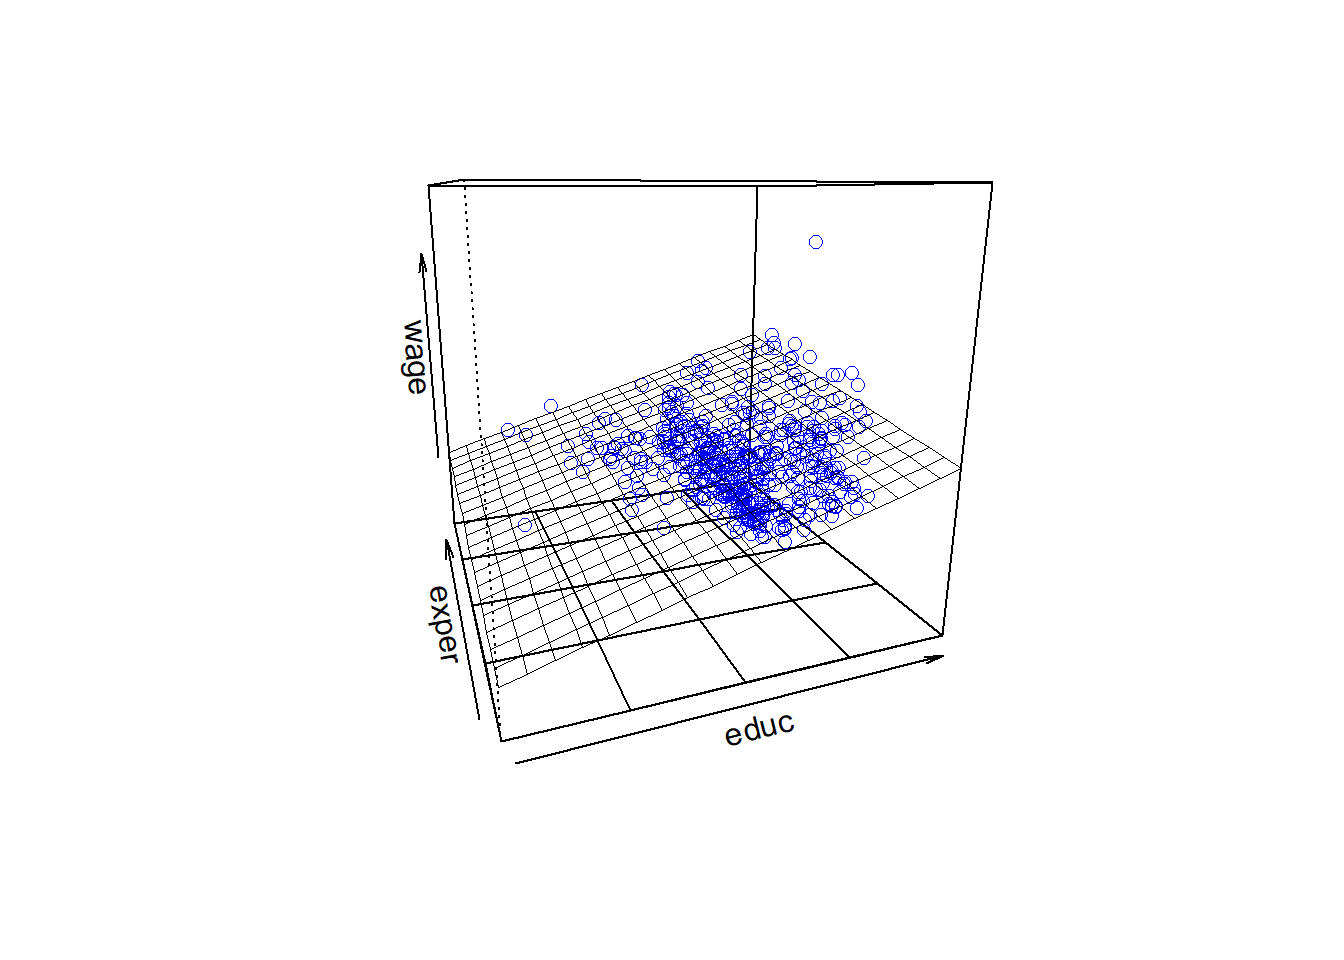
\includegraphics{03_Modelle_Mehr_Variablen_files/figure-latex/Modell2-1.pdf}

Dabei entspricht der Koeffizient \(b_2\) der Zunahme des Gehaltes
\(\hat{y}_i\) wenn sich die Erfahrung \(x_{2i}\) um eine Einheit erhöht
und die Ausbildung \(x_{1i}\) konstant gehalten wird. In nachfolgernder
Tabelle sind die Werte der Vorhersagen des Modells für den vorliegenden
Datensatz auszugsweise dargestellt:

\begin{Shaded}
\begin{Highlighting}[]
\NormalTok{  MinExp    <-}\StringTok{ }\KeywordTok{min}\NormalTok{(CPS85}\OperatorTok{$}\NormalTok{exper)}
\NormalTok{  MaxExp    <-}\StringTok{ }\KeywordTok{max}\NormalTok{(CPS85}\OperatorTok{$}\NormalTok{exper)}
\NormalTok{  RowSeq    <-}\StringTok{ }\KeywordTok{seq}\NormalTok{(}\DataTypeTok{from =} \DecValTok{1}\NormalTok{, }\DataTypeTok{to =}\NormalTok{ MaxExp, }\DataTypeTok{by =} \DecValTok{1}\NormalTok{)}
\NormalTok{  educVon   <-}\StringTok{ }\DecValTok{10}
\NormalTok{  educBis   <-}\StringTok{ }\DecValTok{18}
\NormalTok{  AnzCols   <-}\StringTok{ }\NormalTok{educBis }\OperatorTok{-}\StringTok{ }\NormalTok{educVon }\OperatorTok{+}\StringTok{ }\DecValTok{1}
\NormalTok{  Predicted <-}\StringTok{ }\KeywordTok{matrix}\NormalTok{(}\OtherTok{NA}\NormalTok{, }\DataTypeTok{nrow =}\NormalTok{ MaxExp, }\DataTypeTok{ncol =}\NormalTok{ AnzCols)}
  \ControlFlowTok{for}\NormalTok{ (i }\ControlFlowTok{in} \KeywordTok{seq}\NormalTok{(}\DataTypeTok{from =} \DecValTok{1}\NormalTok{, }\DataTypeTok{to =}\NormalTok{ MaxExp, }\DataTypeTok{by =} \DecValTok{1}\NormalTok{)) \{}
\NormalTok{    new_input     <-}\StringTok{ }\KeywordTok{data.frame}\NormalTok{(}\DataTypeTok{educ =}\NormalTok{ educVon}\OperatorTok{:}\NormalTok{educBis, }\DataTypeTok{exper =}\NormalTok{ i)}
\NormalTok{    Predicted[i,] <-}\StringTok{ }\KeywordTok{predict}\NormalTok{(model_}\DecValTok{2}\NormalTok{, }\DataTypeTok{newdata =}\NormalTok{ new_input)}
\NormalTok{  \}}
\NormalTok{  Predicted           <-}\StringTok{ }\KeywordTok{data.frame}\NormalTok{(}\KeywordTok{seq}\NormalTok{(}\DataTypeTok{from =} \DecValTok{1}\NormalTok{, }\DataTypeTok{to =}\NormalTok{ MaxExp, }\DataTypeTok{by =} \DecValTok{1}\NormalTok{), Predicted)}
  \KeywordTok{colnames}\NormalTok{(Predicted) <-}\StringTok{ }\KeywordTok{c}\NormalTok{(}\StringTok{"Exp"}\NormalTok{, }\StringTok{"Edu10"}\NormalTok{, }\StringTok{"Edu11"}\NormalTok{,}\StringTok{"Edu12"}\NormalTok{, }\StringTok{"Edu13"}\NormalTok{,}
                           \StringTok{"Edu14"}\NormalTok{,}\StringTok{"Edu15"}\NormalTok{, }\StringTok{"Edu16"}\NormalTok{,}\StringTok{"Edu17"}\NormalTok{, }\StringTok{"Edu18"}\NormalTok{)}
\NormalTok{  TabRows2Disp        <-}\StringTok{ }\KeywordTok{c}\NormalTok{(}\DecValTok{1}\OperatorTok{:}\DecValTok{3}\NormalTok{, }\DecValTok{53}\OperatorTok{:}\DecValTok{55}\NormalTok{)}
\NormalTok{  Predicted2Disp      <-}\StringTok{ }\NormalTok{Predicted[TabRows2Disp,]}
  \KeywordTok{row.names}\NormalTok{(Predicted2Disp) <-}\StringTok{ }\OtherTok{NULL}
  \KeywordTok{pander}\NormalTok{(Predicted2Disp, }\DataTypeTok{style =} \StringTok{"rmarkdown"}\NormalTok{)}
\end{Highlighting}
\end{Shaded}

\begin{longtable}[]{@{}cccccccccc@{}}
\toprule
Exp & Edu10 & Edu11 & Edu12 & Edu13 & Edu14 & Edu15 & Edu16 & Edu17 &
Edu18\tabularnewline
\midrule
\endhead
1 & 4.46 & 5.386 & 6.312 & 7.238 & 8.164 & 9.09 & 10.02 & 10.94 &
11.87\tabularnewline
2 & 4.565 & 5.491 & 6.417 & 7.343 & 8.269 & 9.195 & 10.12 & 11.05 &
11.97\tabularnewline
3 & 4.671 & 5.597 & 6.522 & 7.448 & 8.374 & 9.3 & 10.23 & 11.15 &
12.08\tabularnewline
53 & 9.927 & 10.85 & 11.78 & 12.71 & 13.63 & 14.56 & 15.48 & 16.41 &
17.33\tabularnewline
54 & 10.03 & 10.96 & 11.88 & 12.81 & 13.74 & 14.66 & 15.59 & 16.51 &
17.44\tabularnewline
55 & 10.14 & 11.06 & 11.99 & 12.92 & 13.84 & 14.77 & 15.69 & 16.62 &
17.55\tabularnewline
\bottomrule
\end{longtable}

\begin{Shaded}
\begin{Highlighting}[]
  
\NormalTok{  CPS852Disp           <-}\StringTok{ }\KeywordTok{melt}\NormalTok{(Predicted,}
                               \DataTypeTok{id.vars =} \StringTok{"Exp"}\NormalTok{,}
                               \DataTypeTok{measure.vars =} \KeywordTok{c}\NormalTok{(}\StringTok{"Edu10"}\NormalTok{, }\StringTok{"Edu11"}\NormalTok{, }\StringTok{"Edu12"}\NormalTok{,}
                                                \StringTok{"Edu13"}\NormalTok{, }\StringTok{"Edu14"}\NormalTok{,}\StringTok{"Edu15"}\NormalTok{,}
                                                \StringTok{"Edu16"}\NormalTok{, }\StringTok{"Edu17"}\NormalTok{, }\StringTok{"Edu18"}\NormalTok{))}
\NormalTok{  CPS852Disp}\OperatorTok{$}\NormalTok{Exp       <-}\StringTok{ }\KeywordTok{rep}\NormalTok{(}\DecValTok{1}\OperatorTok{:}\DecValTok{55}\NormalTok{, }\DecValTok{9}\NormalTok{)}
  \KeywordTok{colnames}\NormalTok{(CPS852Disp) <-}\StringTok{ }\KeywordTok{c}\NormalTok{(}\StringTok{"Exp"}\NormalTok{, }\StringTok{"Edu"}\NormalTok{, }\StringTok{"WagePred"}\NormalTok{)}
\NormalTok{  p                    <-}\StringTok{ }\KeywordTok{ggplot}\NormalTok{(CPS852Disp, }\KeywordTok{aes}\NormalTok{(}\DataTypeTok{x =}\NormalTok{ Exp, }\DataTypeTok{y =}\NormalTok{ WagePred, }\DataTypeTok{color =}\NormalTok{ Edu)) }\OperatorTok{+}
\StringTok{                          }\KeywordTok{geom_line}\NormalTok{() }\OperatorTok{+}
\StringTok{                          }\KeywordTok{theme_bw}\NormalTok{()}
  \KeywordTok{print}\NormalTok{(p, }\DataTypeTok{comment =} \OtherTok{FALSE}\NormalTok{)}
\end{Highlighting}
\end{Shaded}

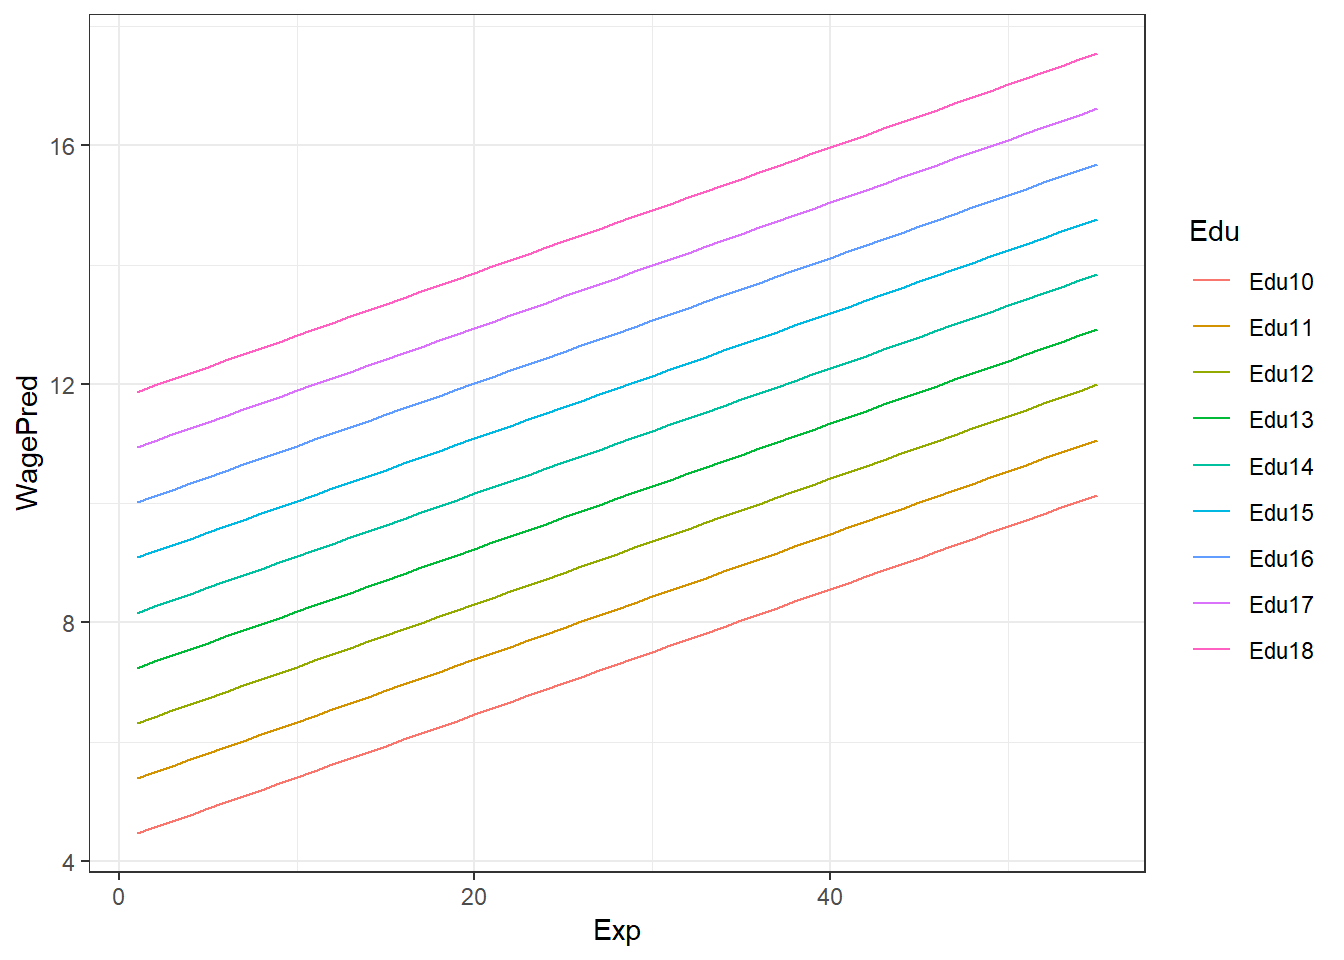
\includegraphics{03_Modelle_Mehr_Variablen_files/figure-latex/Modell2_1-1.pdf}

\subsection*{Modellvergleich}\label{modellvergleich}
\addcontentsline{toc}{subsection}{Modellvergleich}

Ein Modell sollte die Wirklichkeit mit möglichst großer Genauigkeit
abbilden. Bei der Erstellung des Modells wurden aufgrund einer
Stichprobe aus der Grundgesamtheit die Modellparameter (z.B. die
\(b\)'s) bestimmt. Um nun festzustellen, inwieweit das Modell brauchbare
Vorhersagen liefert, sollte man das Modell evaluieren. In den
vorangegangen Beispielen wurden zwei Modelle (\emph{model\_1} und
\emph{model\_2}) erstellt.

Der Vergleich der Modelle ist über den Fehler des jeweiligen Modells
möglich. Je kleiner der Fehler, desto besser bildet das Modell die
beobachteten Werte ab. Im Idealfall (Fehler = 0), würden alle
beobachteten Werte gleich den vorhergesagten Werten sein und damit auf
der Linie liegen.

\begin{Shaded}
\begin{Highlighting}[]
\NormalTok{  M          <-}\StringTok{ }\KeywordTok{data.frame}\NormalTok{(}\DataTypeTok{wage =}\NormalTok{ CPS85}\OperatorTok{$}\NormalTok{wage, }\DataTypeTok{educ =}\NormalTok{ CPS85}\OperatorTok{$}\NormalTok{educ, }\DataTypeTok{exper =}\NormalTok{ CPS85}\OperatorTok{$}\NormalTok{exper)}
\NormalTok{  MV_Data    <-}\StringTok{ }\KeywordTok{data.frame}\NormalTok{(}\DataTypeTok{educ =}\NormalTok{ M}\OperatorTok{$}\NormalTok{educ, }\DataTypeTok{exper =}\NormalTok{ M}\OperatorTok{$}\NormalTok{exper)}
\NormalTok{  MSE_Model1 <-}\StringTok{ }\KeywordTok{round}\NormalTok{(}\KeywordTok{mean}\NormalTok{(}\KeywordTok{resid}\NormalTok{(model_}\DecValTok{1}\NormalTok{)}\OperatorTok{^}\DecValTok{2}\NormalTok{),}\DecValTok{2}\NormalTok{)}
  \CommentTok{#MSE_Model1 <- mean((M$wage - predict(model_1, newdata = MV_Data))^2)}
\NormalTok{  StdResid <-}\StringTok{ }\KeywordTok{rstandard}\NormalTok{(model_}\DecValTok{1}\NormalTok{)}
  \CommentTok{#StdResid <- (resid(model_1)-mean(resid(model_1)))/sd(resid(model_1))}
\NormalTok{  MSE_Model2 <-}\StringTok{ }\KeywordTok{round}\NormalTok{(}\KeywordTok{mean}\NormalTok{((M}\OperatorTok{$}\NormalTok{wage }\OperatorTok{-}\StringTok{ }\KeywordTok{predict}\NormalTok{(model_}\DecValTok{2}\NormalTok{, }\DataTypeTok{newdata =}\NormalTok{ MV_Data))}\OperatorTok{^}\DecValTok{2}\NormalTok{),}\DecValTok{2}\NormalTok{)}
\end{Highlighting}
\end{Shaded}

Der Modellvergleich der obigen Beispiele ergibt für das Modell 1 einen
\(MSE_1 =\) 22.52 und für Modell 2 einen \(MSE_2 =\) 21.04.

Bei diesen Ergebnis lässt sich zunächst nur feststellen, dass der
\(MSE_2\) kleiner als der \(MSE_1\) ist. Ob diese Verringerung des
\(MSE\) von statistischer und/oder praktischer Signifikanz ist, wird im
folgenden noch genauer betrachtet.

Mit einer einfachen ANOVA lässt sich nun auch die statistische
Signifikanz der Änderungen im Fehler bei den verwendeten Modellen
berechnen. Betrachten wir zunächst die statistische Änderung die Modell
1 im Vergleich zum Mittelwertsmodell erzielt:

\begin{Shaded}
\begin{Highlighting}[]
  \CommentTok{# ANOVA Tests auf signifikante Änderungen model_1 vs Mittelwertsmodell}
  \CommentTok{# Berechnung der Quadratsummen für die Regression (educ)}
\NormalTok{  preds_}\DecValTok{1}\NormalTok{            <-}\StringTok{ }\KeywordTok{predict}\NormalTok{(model_}\DecValTok{1}\NormalTok{, }\DataTypeTok{newdata =}\NormalTok{ CPS85)}
\NormalTok{  AnzPred            <-}\StringTok{ }\DecValTok{2} \CommentTok{# b_0 und b_1}
\NormalTok{  SS_Regression_}\DecValTok{1}\NormalTok{    <-}\StringTok{ }\KeywordTok{sum}\NormalTok{((preds_}\DecValTok{1} \OperatorTok{-}\StringTok{ }\KeywordTok{mean}\NormalTok{(preds_}\DecValTok{1}\NormalTok{))}\OperatorTok{^}\DecValTok{2}\NormalTok{)}
\NormalTok{  Zdf_Regression_}\DecValTok{1}\NormalTok{   <-}\StringTok{ }\NormalTok{AnzPred }\OperatorTok{-}\StringTok{ }\DecValTok{1}
\NormalTok{  MSS_Regression_}\DecValTok{1}\NormalTok{   <-}\StringTok{ }\KeywordTok{round}\NormalTok{(SS_Regression_}\DecValTok{1} \OperatorTok{/}\StringTok{ }\NormalTok{Zdf_Regression_}\DecValTok{1}\NormalTok{, }\DecValTok{2}\NormalTok{)}
  \CommentTok{# Berechnung der Quadratsummen des Fehlers (Residuals)}
\NormalTok{  Residuals_}\DecValTok{1}\NormalTok{        <-}\StringTok{ }\NormalTok{CPS85}\OperatorTok{$}\NormalTok{wage }\OperatorTok{-}\StringTok{ }\NormalTok{preds_}\DecValTok{1}
\NormalTok{  SS_Residuals_}\DecValTok{1}\NormalTok{     <-}\StringTok{ }\KeywordTok{sum}\NormalTok{(Residuals_}\DecValTok{1}\OperatorTok{^}\DecValTok{2}\NormalTok{)}
\NormalTok{  Ndf_Residuals_}\DecValTok{1}\NormalTok{    <-}\StringTok{ }\KeywordTok{nrow}\NormalTok{(CPS85) }\OperatorTok{-}\StringTok{ }\NormalTok{AnzPred}
\NormalTok{  MSS_Residuals_}\DecValTok{1}\NormalTok{    <-}\StringTok{ }\KeywordTok{round}\NormalTok{(SS_Residuals_}\DecValTok{1} \OperatorTok{/}\StringTok{ }\NormalTok{Ndf_Residuals_}\DecValTok{1}\NormalTok{, }\DecValTok{2}\NormalTok{)}
  \CommentTok{# Berechnung der Teststatistik}
\NormalTok{  F_Wert             <-}\StringTok{ }\KeywordTok{round}\NormalTok{(MSS_Regression_}\DecValTok{1} \OperatorTok{/}\StringTok{ }\NormalTok{MSS_Residuals_}\DecValTok{1}\NormalTok{, }\DecValTok{2}\NormalTok{)}
  \CommentTok{# Berechnung der totalen Quadratsumme}
\NormalTok{  SS_Total_}\DecValTok{1}\NormalTok{         <-}\StringTok{ }\KeywordTok{sum}\NormalTok{((CPS85}\OperatorTok{$}\NormalTok{wage }\OperatorTok{-}\StringTok{ }\KeywordTok{mean}\NormalTok{(CPS85}\OperatorTok{$}\NormalTok{wage))}\OperatorTok{^}\DecValTok{2}\NormalTok{)}
\NormalTok{  CPS85_Total        <-}\StringTok{ }\KeywordTok{nrow}\NormalTok{(CPS85) }\OperatorTok{-}\StringTok{ }\DecValTok{1}
  \CommentTok{# Vergleich mit den Ergebnissen der ANOVA}
  \KeywordTok{pander}\NormalTok{(}\KeywordTok{anova}\NormalTok{(model_}\DecValTok{1}\NormalTok{))}
\end{Highlighting}
\end{Shaded}

\begin{longtable}[]{@{}cccccc@{}}
\caption{Analysis of Variance Table}\tabularnewline
\toprule
\begin{minipage}[b]{0.19\columnwidth}\centering\strut
~\strut
\end{minipage} & \begin{minipage}[b]{0.07\columnwidth}\centering\strut
Df\strut
\end{minipage} & \begin{minipage}[b]{0.10\columnwidth}\centering\strut
Sum Sq\strut
\end{minipage} & \begin{minipage}[b]{0.12\columnwidth}\centering\strut
Mean Sq\strut
\end{minipage} & \begin{minipage}[b]{0.12\columnwidth}\centering\strut
F value\strut
\end{minipage} & \begin{minipage}[b]{0.13\columnwidth}\centering\strut
Pr(\textgreater{}F)\strut
\end{minipage}\tabularnewline
\midrule
\endfirsthead
\toprule
\begin{minipage}[b]{0.19\columnwidth}\centering\strut
~\strut
\end{minipage} & \begin{minipage}[b]{0.07\columnwidth}\centering\strut
Df\strut
\end{minipage} & \begin{minipage}[b]{0.10\columnwidth}\centering\strut
Sum Sq\strut
\end{minipage} & \begin{minipage}[b]{0.12\columnwidth}\centering\strut
Mean Sq\strut
\end{minipage} & \begin{minipage}[b]{0.12\columnwidth}\centering\strut
F value\strut
\end{minipage} & \begin{minipage}[b]{0.13\columnwidth}\centering\strut
Pr(\textgreater{}F)\strut
\end{minipage}\tabularnewline
\midrule
\endhead
\begin{minipage}[t]{0.19\columnwidth}\centering\strut
\textbf{educ}\strut
\end{minipage} & \begin{minipage}[t]{0.07\columnwidth}\centering\strut
1\strut
\end{minipage} & \begin{minipage}[t]{0.10\columnwidth}\centering\strut
2053\strut
\end{minipage} & \begin{minipage}[t]{0.12\columnwidth}\centering\strut
2053\strut
\end{minipage} & \begin{minipage}[t]{0.12\columnwidth}\centering\strut
90.85\strut
\end{minipage} & \begin{minipage}[t]{0.13\columnwidth}\centering\strut
5.474e-20\strut
\end{minipage}\tabularnewline
\begin{minipage}[t]{0.19\columnwidth}\centering\strut
\textbf{Residuals}\strut
\end{minipage} & \begin{minipage}[t]{0.07\columnwidth}\centering\strut
532\strut
\end{minipage} & \begin{minipage}[t]{0.10\columnwidth}\centering\strut
12023\strut
\end{minipage} & \begin{minipage}[t]{0.12\columnwidth}\centering\strut
22.6\strut
\end{minipage} & \begin{minipage}[t]{0.12\columnwidth}\centering\strut
NA\strut
\end{minipage} & \begin{minipage}[t]{0.13\columnwidth}\centering\strut
NA\strut
\end{minipage}\tabularnewline
\bottomrule
\end{longtable}

Das Ergebnis zeigt uns, dass Modell 1 im Vergleich zum Mittelwertsmodell
zu einer statistisch signifikanten Fehlerreduktion führt. Bei der
händischen Berechnung der Prüfgrößen erhalten wir für die mittlere
Quadratsumme der Regression (also der Varianz der Werte die durch das
Modell vorhergesagt werden) einen Wert von \$MSS\_\{Regression\} = \$
2053.29, welcher ident mit dem Wert der ANOVA-Tabelle ist.

Die restlichen Kennwerte stimmen auch mit dem Ergebnis der ANOVA überein
(\(MSS_{Residual}\) = 22.6, F(1,532) = 90.85).

Wird das Modell 1 erweitert (auf Modell 2), stellt sich die Frage, ob
diese Erweiterung im statistischen Sinn zu einer signifikanten
Verbesserung führt. Bei diesem Vergleich wird nun die Änderung (Change
Statistic) zwischen Modell 1 und Modell 2 auf Signifikanz geprüft.

\begin{Shaded}
\begin{Highlighting}[]
  \CommentTok{# ANOVA Tests auf signifikante Änderungen model_1 vs model_2 (Änderung signifikant?)}
  \KeywordTok{pander}\NormalTok{(}\KeywordTok{anova}\NormalTok{(model_}\DecValTok{1}\NormalTok{, model_}\DecValTok{2}\NormalTok{))}
\end{Highlighting}
\end{Shaded}

\begin{longtable}[]{@{}cccccc@{}}
\caption{Analysis of Variance Table}\tabularnewline
\toprule
\begin{minipage}[b]{0.10\columnwidth}\centering\strut
Res.Df\strut
\end{minipage} & \begin{minipage}[b]{0.09\columnwidth}\centering\strut
RSS\strut
\end{minipage} & \begin{minipage}[b]{0.06\columnwidth}\centering\strut
Df\strut
\end{minipage} & \begin{minipage}[b]{0.14\columnwidth}\centering\strut
Sum of Sq\strut
\end{minipage} & \begin{minipage}[b]{0.09\columnwidth}\centering\strut
F\strut
\end{minipage} & \begin{minipage}[b]{0.13\columnwidth}\centering\strut
Pr(\textgreater{}F)\strut
\end{minipage}\tabularnewline
\midrule
\endfirsthead
\toprule
\begin{minipage}[b]{0.10\columnwidth}\centering\strut
Res.Df\strut
\end{minipage} & \begin{minipage}[b]{0.09\columnwidth}\centering\strut
RSS\strut
\end{minipage} & \begin{minipage}[b]{0.06\columnwidth}\centering\strut
Df\strut
\end{minipage} & \begin{minipage}[b]{0.14\columnwidth}\centering\strut
Sum of Sq\strut
\end{minipage} & \begin{minipage}[b]{0.09\columnwidth}\centering\strut
F\strut
\end{minipage} & \begin{minipage}[b]{0.13\columnwidth}\centering\strut
Pr(\textgreater{}F)\strut
\end{minipage}\tabularnewline
\midrule
\endhead
\begin{minipage}[t]{0.10\columnwidth}\centering\strut
532\strut
\end{minipage} & \begin{minipage}[t]{0.09\columnwidth}\centering\strut
12023\strut
\end{minipage} & \begin{minipage}[t]{0.06\columnwidth}\centering\strut
NA\strut
\end{minipage} & \begin{minipage}[t]{0.14\columnwidth}\centering\strut
NA\strut
\end{minipage} & \begin{minipage}[t]{0.09\columnwidth}\centering\strut
NA\strut
\end{minipage} & \begin{minipage}[t]{0.13\columnwidth}\centering\strut
NA\strut
\end{minipage}\tabularnewline
\begin{minipage}[t]{0.10\columnwidth}\centering\strut
531\strut
\end{minipage} & \begin{minipage}[t]{0.09\columnwidth}\centering\strut
11233\strut
\end{minipage} & \begin{minipage}[t]{0.06\columnwidth}\centering\strut
1\strut
\end{minipage} & \begin{minipage}[t]{0.14\columnwidth}\centering\strut
790.6\strut
\end{minipage} & \begin{minipage}[t]{0.09\columnwidth}\centering\strut
37.37\strut
\end{minipage} & \begin{minipage}[t]{0.13\columnwidth}\centering\strut
1.893e-09\strut
\end{minipage}\tabularnewline
\bottomrule
\end{longtable}

Zum Verständnis dieser Statistik greifen wir kurz zurück auf die
verschiedenen Möglichkeiten der Berechnung von Korrelationskoeffizienten
zurück. Diese sind:

\begin{enumerate}
\def\labelenumi{\arabic{enumi}.}
\tightlist
\item
  Pearson Korrelationskoeffizient (\(r_{xy}\)): entspricht der Kovarianz
  der \(z\)-transformierten Variablen.
\item
  Partielle Korrealtionskoeffizient (\(r_{xy \cdot z}\)): ist die
  bivariate Korrelation zweier Variablen, welche mittels linearer
  Regression vom Einfluss einer Drittvariablen bereinigt wurden.
  3.Semipartialkorrelation (\(sr_{k \cdot x_j}\)): zwischen Kriterium
  und dem \(j\)-ten Prädiktor ergibt sich als Korrelation von \(y\) mit
  dem Residuum \(x_j^*\) der linearen Regression des \(j\)-ten
  Prädiktors auf den anderen Prädiktor. Mit anderen Worten, die
  Semipartialkorrelation gibt den alleinigen Beitrag eines Prädiktors
  \(x_j\) (bereinigt um die gemeinsamen Anteile mit den restlichen
  Prädiktoren) am Kriterium an. Das Quadrat dieses Koeffizienten wird
  unter anderm auch als Nützlichkeit des Prädiktors \(U_k\) bezeichnet
  und findet sich z.B. in SPSS als \(R^2_{change}\) wieder. Formal:
  \(sr_{k \cdot 12 \cdots (k-1)}^2 = R_{y, 12 \cdots k}^2 - R_{y, 12 \cdots k-1}^2\)
\end{enumerate}

\begin{Shaded}
\begin{Highlighting}[]
  \CommentTok{# Korrelationen, Paritial- und Semipartialkorrelationen}
\NormalTok{  Korr_Data      <-}\StringTok{ }\KeywordTok{data.frame}\NormalTok{(}\DataTypeTok{wage =}\NormalTok{ M}\OperatorTok{$}\NormalTok{wage, }\DataTypeTok{educ =}\NormalTok{ M}\OperatorTok{$}\NormalTok{educ, }\DataTypeTok{exper =}\NormalTok{ M}\OperatorTok{$}\NormalTok{exper)}
\NormalTok{  PearsonKorr    <-}\StringTok{ }\KeywordTok{cor}\NormalTok{(Korr_Data)}
\NormalTok{  ModVgl_Korr    <-}\StringTok{ }\KeywordTok{pander}\NormalTok{(PearsonKorr)}
\NormalTok{  R2Change_mod_}\DecValTok{1}\NormalTok{ <-}\StringTok{ }\NormalTok{PearsonKorr[}\DecValTok{2}\NormalTok{]}\OperatorTok{^}\DecValTok{2}
  \CommentTok{# Partial Korrelation zwischen "wage" und "educ" gegeben "exper"}
\NormalTok{  PartKorr_}\DecValTok{1}\NormalTok{       <-}\StringTok{ }\KeywordTok{pcor.test}\NormalTok{(Korr_Data}\OperatorTok{$}\NormalTok{wage, Korr_Data}\OperatorTok{$}\NormalTok{educ, Korr_Data}\OperatorTok{$}\NormalTok{exper)}
\NormalTok{  ModVgl_ParKorr_}\DecValTok{1}\NormalTok{ <-}\StringTok{ }\KeywordTok{pander}\NormalTok{(PartKorr_}\DecValTok{1}\NormalTok{)}
  \CommentTok{# Partial Korrelation zwischen "wage" und "exper" gegeben "educ"}
\NormalTok{  PartKorr_}\DecValTok{2}\NormalTok{       <-}\StringTok{ }\KeywordTok{pcor.test}\NormalTok{(Korr_Data}\OperatorTok{$}\NormalTok{wage, Korr_Data}\OperatorTok{$}\NormalTok{exper, Korr_Data}\OperatorTok{$}\NormalTok{educ)}
\NormalTok{  ModVgl_ParKorr_}\DecValTok{2}\NormalTok{ <-}\StringTok{ }\KeywordTok{pander}\NormalTok{(PartKorr_}\DecValTok{2}\NormalTok{)}
  \CommentTok{# Semi-Partial (part) Korrelation zwischen "wage" und "educ" gegeben "exper"}
\NormalTok{  SemiPartKorr_}\DecValTok{1}\NormalTok{      <-}\StringTok{ }\KeywordTok{spcor.test}\NormalTok{(Korr_Data}\OperatorTok{$}\NormalTok{wage, Korr_Data}\OperatorTok{$}\NormalTok{educ, Korr_Data}\OperatorTok{$}\NormalTok{exper)}
\NormalTok{  ModVgl_SemParKorr_}\DecValTok{1}\NormalTok{ <-}\StringTok{ }\KeywordTok{pander}\NormalTok{(SemiPartKorr_}\DecValTok{1}\NormalTok{)}
  \CommentTok{# Semi-Partial (part) Korrelation zwischen "wage" und "exper" gegeben "edu"}
\NormalTok{  SemiPartKorr_}\DecValTok{2}\NormalTok{      <-}\StringTok{ }\KeywordTok{spcor.test}\NormalTok{(Korr_Data}\OperatorTok{$}\NormalTok{wage, Korr_Data}\OperatorTok{$}\NormalTok{exper, Korr_Data}\OperatorTok{$}\NormalTok{educ)}
\NormalTok{  ModVgl_SemParKorr_}\DecValTok{1}\NormalTok{ <-}\StringTok{ }\KeywordTok{pander}\NormalTok{(SemiPartKorr_}\DecValTok{2}\NormalTok{)}
\NormalTok{  R2Change_mod_}\DecValTok{2}\NormalTok{      <-}\StringTok{ }\KeywordTok{round}\NormalTok{(SemiPartKorr_}\DecValTok{2}\OperatorTok{$}\NormalTok{estimate}\OperatorTok{^}\DecValTok{2}\NormalTok{,}\DecValTok{3}\NormalTok{)}
  \KeywordTok{pander}\NormalTok{(}\KeywordTok{summary}\NormalTok{(model_}\DecValTok{2}\NormalTok{))}
\end{Highlighting}
\end{Shaded}

\begin{longtable}[]{@{}ccccc@{}}
\toprule
\begin{minipage}[b]{0.21\columnwidth}\centering\strut
~\strut
\end{minipage} & \begin{minipage}[b]{0.13\columnwidth}\centering\strut
Estimate\strut
\end{minipage} & \begin{minipage}[b]{0.16\columnwidth}\centering\strut
Std. Error\strut
\end{minipage} & \begin{minipage}[b]{0.12\columnwidth}\centering\strut
t value\strut
\end{minipage} & \begin{minipage}[b]{0.13\columnwidth}\centering\strut
Pr(\textgreater{}\textbar{}t\textbar{})\strut
\end{minipage}\tabularnewline
\midrule
\endhead
\begin{minipage}[t]{0.21\columnwidth}\centering\strut
\textbf{(Intercept)}\strut
\end{minipage} & \begin{minipage}[t]{0.13\columnwidth}\centering\strut
-4.904\strut
\end{minipage} & \begin{minipage}[t]{0.16\columnwidth}\centering\strut
1.219\strut
\end{minipage} & \begin{minipage}[t]{0.12\columnwidth}\centering\strut
-4.024\strut
\end{minipage} & \begin{minipage}[t]{0.13\columnwidth}\centering\strut
6.564e-05\strut
\end{minipage}\tabularnewline
\begin{minipage}[t]{0.21\columnwidth}\centering\strut
\textbf{educ}\strut
\end{minipage} & \begin{minipage}[t]{0.13\columnwidth}\centering\strut
0.926\strut
\end{minipage} & \begin{minipage}[t]{0.16\columnwidth}\centering\strut
0.0814\strut
\end{minipage} & \begin{minipage}[t]{0.12\columnwidth}\centering\strut
11.37\strut
\end{minipage} & \begin{minipage}[t]{0.13\columnwidth}\centering\strut
5.563e-27\strut
\end{minipage}\tabularnewline
\begin{minipage}[t]{0.21\columnwidth}\centering\strut
\textbf{exper}\strut
\end{minipage} & \begin{minipage}[t]{0.13\columnwidth}\centering\strut
0.1051\strut
\end{minipage} & \begin{minipage}[t]{0.16\columnwidth}\centering\strut
0.0172\strut
\end{minipage} & \begin{minipage}[t]{0.12\columnwidth}\centering\strut
6.113\strut
\end{minipage} & \begin{minipage}[t]{0.13\columnwidth}\centering\strut
1.893e-09\strut
\end{minipage}\tabularnewline
\bottomrule
\end{longtable}

\begin{longtable}[]{@{}cccc@{}}
\caption{Fitting linear model: wage \textasciitilde{} educ +
exper}\tabularnewline
\toprule
\begin{minipage}[b]{0.18\columnwidth}\centering\strut
Observations\strut
\end{minipage} & \begin{minipage}[b]{0.27\columnwidth}\centering\strut
Residual Std. Error\strut
\end{minipage} & \begin{minipage}[b]{0.10\columnwidth}\centering\strut
\(R^2\)\strut
\end{minipage} & \begin{minipage}[b]{0.20\columnwidth}\centering\strut
Adjusted \(R^2\)\strut
\end{minipage}\tabularnewline
\midrule
\endfirsthead
\toprule
\begin{minipage}[b]{0.18\columnwidth}\centering\strut
Observations\strut
\end{minipage} & \begin{minipage}[b]{0.27\columnwidth}\centering\strut
Residual Std. Error\strut
\end{minipage} & \begin{minipage}[b]{0.10\columnwidth}\centering\strut
\(R^2\)\strut
\end{minipage} & \begin{minipage}[b]{0.20\columnwidth}\centering\strut
Adjusted \(R^2\)\strut
\end{minipage}\tabularnewline
\midrule
\endhead
\begin{minipage}[t]{0.18\columnwidth}\centering\strut
534\strut
\end{minipage} & \begin{minipage}[t]{0.27\columnwidth}\centering\strut
4.599\strut
\end{minipage} & \begin{minipage}[t]{0.10\columnwidth}\centering\strut
0.202\strut
\end{minipage} & \begin{minipage}[t]{0.20\columnwidth}\centering\strut
0.199\strut
\end{minipage}\tabularnewline
\bottomrule
\end{longtable}

Im vorliegenden Beispiel sind daher die beiden Nützlichkeitsmaße
\(U_{educ}\) = 0.146 und \(U_{exper}\) = 0.056 von Interesse. Ersteres
bedeutet, dass die Varianzaufklärung aufgrund der Verwendung der
Variablen \emph{educ} 14.6\% ist. Wird im Modell dann noch der Prädiktor
\emph{exper} aufgenommen, werden zusätzliche 5.6\% an Varianz des
Kriteriums wage erklärt. Insgesamt werden somit \(R^2 = 0.202\) oder
20.2\% der Varianz des Kriteriums erklärt. Der Test
(\(t(531) = 11.37, p< .001\)) bestätigt für den Prädiktor \emph{educ},
sowie (\(t(531) = 6.11, p<.001\)) für den Prädiktor \emph{exper} die
statistische Signifikanz.

\hypertarget{aufgabe-mlr-1}{\subsection*{Aufgabe MLR
1}\label{aufgabe-mlr-1}}
\addcontentsline{toc}{subsection}{Aufgabe MLR 1}

Öffne ein neues R-Script und kopiere die bereits bekannte Kopfzeile in
diese Datei. Speichere anschließend das Skript unter dem Namen
\emph{SLR\_Aufgabe2.R}. Bearbeite nun folgende Aufgabenstellungen:

\begin{itemize}
\tightlist
\item
  Lade die Datei ``\emph{Album Sales 2.dat}''
\item
  erstelle ein lineares Modell zur Vorhersage der Verkaufszahlen
  (\emph{sales}) durch die Variable \emph{adverts}.
\item
  erstelle ein weiteres lineares Modell zur Vorhersage der
  Verkaufszahlen (\emph{sales}) durch die Variable \emph{adverts},
  \emph{airplay} und \emph{attract}.
\item
  Zeige die Ergebnisse des ersten Modells an.
\item
  Zeige die Ergebnisse des zweiten Modells an.
\item
  Vergleiche die beiden Modelle mit einer ANOVA und interpretiere die
  Ergebnisse.
\item
  Berechne zur Überprüfung der Multikolinearität den Kennwert \emph{Tol}
  und \emph{VIF} (verwende die Funktion \emph{vif()}. Hinweis: die
  Toleranz ist der Kehrwert von \emph{VIF})
\end{itemize}

\protect\hyperlink{aufgabe-mlr-1-lsg}{Lösung Aufgabe MLR 1}

\subsection*{Wahl relevanter
Prädiktoren}\label{wahl-relevanter-pradiktoren}
\addcontentsline{toc}{subsection}{Wahl relevanter Prädiktoren}

Eine wichtige Frage bei der Modellerstellung betrifft die Wahl der
besten Prädiktoren. Prinzipiell muss bereits im Vorfeld der
statistischen Analyse bestimmt werden, welche Merkmale für die
Modellierung der abhängigen Variablen am geeignetsten sind. Ausreichende
theoretische und praktischen Kenntnisse sind daher unbedingt
erforderlich. Die Erfassung von potentiellen Prädiktoren ist stets mit
zeitlichen und/oder finanziellen Aufwand verbunden. Prädiktoren sind
dann gut geeignet, wenn Sie folgende Eigenschaften erfüllen:

\begin{enumerate}
\def\labelenumi{\arabic{enumi}.}
\tightlist
\item
  jeder Prädiktor erklärt möglichst viel der Variabilität des
  Kriteriums.
\item
  die Prädiktoren (z.B. \(x_1\) und \(x_2\)) sind im günstigsten Fall
  voneinander unabhängig (\(r(x_1,x_2) \approx 0\))
\end{enumerate}

Diese Eigenschaft kann man durch eine einfache paarweise Korrelation
prüfen. Vor allem wenn die zweite Eigenschaft nicht gegeben ist, also
wenn einen hohe Korrelationen zwischen zwei Prädiktoren vorliegt, wird
es bei der Modellierung zu maßgeblichen Problemen (Multikollinearität)
kommen (siehe:
\protect\hyperlink{voraussetzungen-der-multiplen-regression}{Voraussetzungen
der multiplen Regression}.

Neben der Frage nach der Güte einzelner Prädiktoren ist es auch wichtig
sich Gedanken über die Anzahl der zu verwendenden Prädiktoren zu machen.
Einerseits führt trivialerweise eine höhere Anzahl von Prädiktoren auch
zu einer besseren Aufklärung der Varianz im Kriterium. Ausgenommen von
Prädiktoren die in keiner Beziehung zum Kriterium stehen, wird jeder
zusätzliche Prädiktor mehr oder weniger der verbleibenden Varianz
erklären. In den meisten Fällen ist es aber aus zeitlichen/finanziellen
oder sonstigen Gründen nicht sinnvoll, eine möglichst große Menge an
Prädiktorvariablen zu erheben.

Werden zu viele erklärende Variablen zur Spezifizierung eines Modells
verwendet, wird die tatsächliche (geringere) Anpassungsgüte
verschleiert. Das Modell wird zwar besser auf die Daten der Stichprobe
angepasst, allerdings besteht aufgrund fehlender Generalität keine
Übertragbarkeit auf die Grundgesamtheit. Grundsätzlich sollte wie
bereits erwähnt die Wahl der Prädiktoren auf theoretisch und praktisch
fundierten Grundlagen erfolgen. Welche der zur Verfügung stehenden
Prädiktoren im Endeffekt für das Modell verwendet werden, kann anhand
der Modellvergleiche auch im statistischen Sinn evaluiert werden.

Bei der bisher besprochenen Vorgehensweise der Modellerstellung obliegt
es dem Analysten, die zu verwendenden Prädiktoren zu bestimmen. Eine
weitere Möglichkeit bietet die sogenannte sequentielle Vorgehensweise,
bei der die Ein- und Ausschlusskriterien für Prädiktoren durch
statistische Kriterien getroffen werden.

\subsection*{Sequentielle
Modellbildung}\label{sequentielle-modellbildung}
\addcontentsline{toc}{subsection}{Sequentielle Modellbildung}

In manchen Fällen sind nicht ausreichende theoretische Grundlagen und
Erfahrungswerte bezüglich der Wirksamkeit und Wichtigkeit von
Prädiktoren vorhanden. In solchen Fällen kann ein exploratives Vorgehen
bei der Modellerstellung sehr hilfreich sein. Die nachfolgend
beschriebene sequentielle Modellierung entspricht einem solchen Ansatz.

Bei der sequentiellen Modellbildung wird ein Modell schrittweise mit
unabhängigen Variablen erweitert. In der Regel wird jene Variable, die
das \(R^2\) am meisten vergrößert und damit die Vorhersage am meisten
verbessert hinzugefügt.

Abhängig von der Anzahl der verfügbaren Prädiktoren wird die Bildung
neuer Modelle entweder abgebrochen, wenn weitere Variablen keinen
weiteren statistischen signifikanten Beitrag zur Varianzaufklärung mehr
leisten, oder wenn keine weiteren Variablen zur Verfügung stehen.

Aufgrund der statistischen (maschinellen) Entscheidung über die
Verwendung von Prädiktoren, wird diese Vorgehensweise vielfach
kritisiert. Nehmen wir in einem sehr einfachen Beispiel einmal an, es
stehen 2 Prädiktoren (\(x_1, x_2\)) zur Vorhersage der abhängigen
Variablen zur Verfügung. Der Prädiktor \(x_1\) klärt geringfügig weniger
Varianz des Kriteriums auf als Prädiktor \(x_2\), ersterer ist aber
inhaltlich sinnvoller, leichter zu interpretiern und vor allem weit
kostengünstiger zu erfassen. Bei der sequentiellen Methode könnte aber
aufgrund des Abbruchkriteriums (Signifikanz des Beitrags) genau dieser
Prädiktor vom Modell ausgeschlossen werden.

Bei der sequentiellen Methode unterscheidet man noch unterschiedliche
Vorgehensweisen hinsichtlich des Hinzufügens/Entfernens von Variablen:

\begin{enumerate}
\def\labelenumi{\arabic{enumi}.}
\tightlist
\item
  Schrittweise (STEPWISE): Diese Methode ist ähnlich wie
  ``Vorwärts''-Selektion, es wird aber zusätzlich bei jedem Schritt
  getestet, ob die am wenigsten ``nützliche'' Variable entfernt werden
  soll.
\item
  Vorwärts-Selektion (FORWARD): Die Variablen werden sequenziell in das
  Modell aufgenommen. Diejenige unabhängige Variable, welche am
  stärksten mit der abhängigen Variable korreliert wird zuerst zum
  Modell hinzugefügt. Dann wird jene der verbleibenden Variablen
  hinzugefügt, die die höchste partielle Korrelation mit der abhängigen
  Variablen aufweist. Dieser Schritt wird wiederholt, bis sich die
  Modellgüte (R-Quadrat) nicht weiter signifikant erhöht oder alle
  Variablen ins Modellaufgenommen worden sind.
\item
  Rückwärts-Elimination (BACKWARD): Zunächst sind alle Variablen im
  Regressionsmodell enthalten und werden anschließend sequenziell
  entfernt. Schrittweise wird immer diejenige unabhängige Variable
  entfernt, welche die kleinste partielle Korrelation mit der abhängigen
  Variable aufweist, bis entweder keine Variablen mehr im Modell sind
  oder keine die verwendeten Ausschlusskriterien erfüllen. Im
  Unterschied zur STEPWISE-Methode wird nicht mehr geprüft, ob die am
  wenigsten nützliche Variable entfernt werden soll - diese bleibt somit
  im Modell!
\end{enumerate}

Diese Methoden unterscheiden sich von der sogenannten Einschlussmethode
(ENTER), bei der alle Variablen gleichzeitig in das Modell eingefügt
werden. Diese Methode wird angewendet, wenn das Modell auf theoretischen
Überlegungen basiert. Das heißt, sie eignet sich um Theorien zu testen,
während die übrigen Methoden eher im Rahmen explorativer Studien
eingesetzt werden.

\subsection*{Modellvergleich durch AIC}\label{modellvergleich-durch-aic}
\addcontentsline{toc}{subsection}{Modellvergleich durch AIC}

Nach einer (explorativen) Analyse der Daten und der Wahl einer passenden
Modellklasse, geht es darum das bestmögliche Modell zu den vorliegenden
Daten zu finden (siehe FUB). Daher stellt sich die Frage, was
``bestmögliches'' Modell bedeutet und wie ein solches bestimmt werden
kann. In diesem Zusammenhang wird der Gedanke aufgegriffen, dass mit
keinem Regressionsmodell die Realität eins zu eins abgebildet werden
kann. Nimmt man zu viele erklärende Variablen auf, läuft man in Gefahr
das Modell zu ``overfitten'' (überanpassen). Ein überangepasstes Modell
erklärt die zum Schätzen verwendete abhängige Variable meist sehr gut,
schneidet jedoch in der Vorhersage von Daten außerhalb der verwendeten
Stichprobe häufig schlecht ab. Auf der anderen Seite kann ein Modell
auch ``underfitted'' sein, d.h. die aufgenommenen unabhängigen Variablen
können die abhängige Variable nur sehr unzureichend erklären.

Das Thema der Modellselektion ist ein allgegenwärtiges in der Statistik/
Regressionsanalyse. Dennoch gibt es keine absoluten, objektiven
Kriterien anhand derer entschieden werden kann, ob das eine oder das
andere Modell gewählt werden sollte. Vielmehr existieren viele
verschiedene Verfahren, die versuchen zwischen möglichst viel
Erklärungsgehalt des Modells und möglichst wenig Komplexität (siehe dazu
\href{https://de.wikipedia.org/wiki/Ockhams_Rasiermesser}{Ockhams
Rasiermesser}) abzuwägen.

In einem Artikel von (Yamashita \protect\hyperlink{ref-Yamashita}{2007})
wurden folgende Methoden:

\begin{enumerate}
\def\labelenumi{\alph{enumi}.}
\tightlist
\item
  Partial F
\item
  Partial Correlation
\item
  Semi-Partial Correlation
\item
  Akaike Information Criteria (AIC)
\end{enumerate}

für den Vergleich von Regressionsmodellen untersucht. Die Autoren
schließen aus den Ergebnissen ihrer Untersuchung, dass alle Methoden zu
den gleichen Ergebnissen, d.h. zur gleichen Modellentscheidung gelangen.
Da aber der AIC einerseits leicht zu interpretieren und andererseits
auch auf nichtlineare Modelle und Modelle die auf nicht normalverteilten
Daten beruhen zu erweitern ist, wird die Anwendung dieses Kriteriums
empfohlen.

Das AIC dient also dazu, verschiedene Modellkandidaten zu vergleichen.
Dies geschieht anhand des Wertes der log-Likelihood, der umso größer
ist, je besser das Modell die abhängige Variable erklärt. Um nicht
komplexere Modelle als durchweg besser einzustufen wird neben der
log-Likelihood noch die Anzahl der geschätzten Parameter als Strafterm
mitaufgenommen.

\begin{equation} 
  AIC_k = 2 \cdot |k| - 2\cdot \hat{L}_k
  \label{eq:AIC}
\end{equation}

In der Formel steht \(k\) für die Anzahl der im Modell enthaltenen
Parameter und \(\hat{L}_k\) für den Wert der log-Likelihoodfunktion.

\textbf{Das Modell mit dem kleinsten AIC wird bevorzugt.}

Das AIC darf nicht als absolutes Gütemaß verstanden werden. Auch das
Modell, welches vom Akaike Kriterium als bestes ausgewiesen wird, kann
eine sehr schlechte Anpassung an die Daten aufweisen. Die Anpassung ist
lediglich besser als in den Alternativmodellen.

Die praktische Bedeutung soll anhand eines einfachen Beispiels und der
Verwendung des Kriteriums bei unseren Beispieldaten erläutert werden.

Nehmen wir an, dass drei Modellvergleiche (mod\_1,mod\_2,mod\_3)
folgende AIC-Werte ergeben haben:

\(AIC_1 = 100, AIC_2 = 102, AIC_3 = 110\). Berechnet man
\(e^{(AIC_{min} - AIC_i)/2}\), kann das Ergebnis folgendermaßen
interpretiert werden:

\begin{itemize}
\tightlist
\item
  Beim \emph{mod\_2} ist es um das \(e^{(100-102)/2} = 0.368\)-fache
  wahrscheinlicher den Informationsverlust zu verringern als bei Modell
  1 (\emph{mod\_1}).
\item
  Beim \emph{mod\_3} ist es um das \(e^{(100-110)/2} = 0.007\)-fache
  wahrscheinlicher den Informationsverlust zu verringern als bei Modell
  1 (\emph{mod\_1}).
\end{itemize}

Bei diesem Beispiel würde man also \emph{mod\_3} für weitere
Betrachtungen ausschließen. Nachdem aber die Modelle \emph{mod\_1} und
\emph{mod\_2} sehr nahe beisammen liegen, ist es mit den vorliegenden
Daten nicht möglich, eine klare Entscheidung für eines der beiden
Modelle zu treffen.

Man könnte durchaus noch zusätzliche Daten erheben um dadurch eventuell
eine klarere Trennung der beiden Modelle (\emph{mod\_1}, \emph{mod\_2})
zu erkennen. Ist das nicht möglich, könnte man beide Modelle mit der
relativen likelihood gewichten und auf eine statistische Signifikanz
testen, oder davon ausgehen, dass mit den vorliegenden Daten eine
Modellwahl eben nicht eindeutig zu treffen ist.

\subsection*{Kreuzvalidierung}\label{kreuzvalidierung}
\addcontentsline{toc}{subsection}{Kreuzvalidierung}

Betrachten wir im Folgenden ein Modell (\emph{mod\_1}) mit den
Prädiktoren \emph{sector} (Berufsgruppe), \emph{exper} (Erfahrung),
sowie das um den Prädiktor \emph{age} (Alter) erweiterte Model
(\emph{mod\_2}).

Die Vorhergehensweise bei der Kreuzvalidierung ist relativ simpel:

\begin{enumerate}
\def\labelenumi{\arabic{enumi}.}
\tightlist
\item
  Erstelle ein/mehrere Modell(e) und berechne die jeweiligen
  Modellparameter \(b_i^j\) (mit \(j = j\)-tes Modell und \(i = i\)'ter
  Parameter) mit einer Teilmenge der zur Verfügung stehenden Daten (z.B.
  \emph{Training\_Data} \(\subset\) \emph{DF}).
\item
  Verwende die restlichen Daten um mit den entsprechenden Modellen
  Vorhersagen zu berechnen.
\item
  Berechne die Differenz der beobachteten Daten und der vorhergesagten
  Daten. Diese Differenz entspricht dem Fehler des Modells
  (\(\rightarrow \epsilon_i\)).
\item
  Berechne den mittleren quadratischen Fehler der Differenzen.
\end{enumerate}

\subsection*{Voraussetzungen MLR}\label{voraussetzungen-mlr}
\addcontentsline{toc}{subsection}{Voraussetzungen MLR}

Folgende Voraussetzungen müssen/sollten bei der linearen Modellierung
mit mehreren Prädiktoren erfüllt sein, damit die Ergebnisse auch
sinnvoll interpretiert werden können (Bemerkung: im folgenden sei die
abhängige Variable \(y\) und die Prädiktoren mit den Zahlen
\({1, 2, \cdots, k}\) bezeichnet):

\begin{enumerate}
\def\labelenumi{\arabic{enumi}.}
\tightlist
\item
  \textbf{Lineare Beziehung} zwischen den Variablen (keine Ausreißer):
  eine einfache Prüfung erfolgt visuell mit Streudiagrammen, wobei alle
  Beziehungen, also
  \(r_{y\cdot1}, r_{y\cdot2}, \cdots, r_{y\cdot k}, \cdots, r_{1\cdot2}, r_{1\cdot k}, \cdots, r_{(k-1)\cdot k}\)
  zu betrachten sind!
\item
  \textbf{Varianzgleichheit der Residuen} (Homoskädasdizität): auch
  diese Vorausstung kann visuell geprüft werden. Dabei wird ein
  Streudiagramm der Residuen erstellt, in welchem auf der x-Achse die
  standardisierten vorhergesagten Werte und auf der y-Achse doe
  standardisierten Residuen aufgetragen werden. Heteroskedastizität
  liegt vor, wenn die Punktewolke nicht gleichverteilt um die Gerade
  liegen!
\end{enumerate}

\begin{figure}
\centering
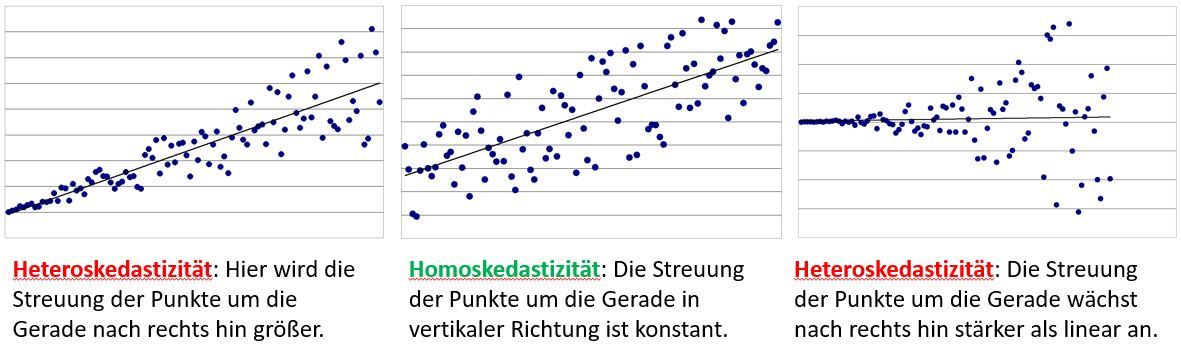
\includegraphics[width=0.80000\textwidth]{Images/Homoskedastizitaet.JPG}
\caption{\textbf{Abbildung 3}: Homoskedastizität
vs.~Heteroskedastizität}
\end{figure}

Bekannte Verfahren, um die Nullhypothese „Homoskedastizität`` zu
überprüfen sind der:

\begin{verbatim}
    * Levene-Test
    * Goldfeld-Quandt-Test
    * White-Test
    * Glejser-Test
    * RESET-Test
    * Breusch-Pagan-Test
\end{verbatim}

\begin{enumerate}
\def\labelenumi{\arabic{enumi}.}
\setcounter{enumi}{2}
\item
  \textbf{Normalverteilung der Residuen}: mittels Histogramm der Fehler
  zu prüfen - sollte halbwegs normalverteilt sein mit einem
  Erwartungswert des Fehlers \(E(\varepsilon) = 0\).
\item
  \textbf{Unabhängigkeit der Residuen} (keine Autokorrelation): verletzt
  wird diese Voraussetzung, wenn aufeinanderfolgende Werte abhängig sind
  (z.B. auf einen hohen Wert folgt ein hoher Wert, etc.). Vor allem bei
  Längsschnittdaten ein Thema, bei welchen die Prüfung durch die
  Durbin-Watson-Methode empfohlen wird. Es gilt:
  \(d = \frac{\sum_{i} (e_i - e_{i-1})^2}{\sum_{i} (e_i)^2}\) mit
  \(d \approx 2\), Werte zwischen \(1.5 < d < 2.5\) sind noch
  akzeptabel.
\item
  \textbf{Vollständig spezifizierte Modelle}: werden maßgebliche
  Prädiktoren nicht im Modell berücksichtigt, wird es auch kaum
  gelingen, die Varianz des Kriteriums zufriedenstellend zu erklären.
  Andererseits bewirken Modelle mit vielen Prädiktoren, dass die
  \(\beta\)-Gewichte entsprechend klein werden. Bei derartigen
  Gegebenheiten ist die Stichprobe entsprechend groß zu wählen.
\item
  \textbf{Keine Multikollinearität}: Multikollinearität bedeutet, dass
  Prädiktoren existieren, die hoch miteinander korrelieren (z.B.
  \(r_{1\cdot2} > 0.8\)). Damit wird es für das Modell schwer, den
  jeweiligen Beitrag den Prädiktoren zuzuordnen. Besteht rein das
  Interesse an maximaler Varianzaufklärung des Kriteriums, ist eine hohe
  Multikollinearität zu vernachlässigen - die \(\beta\)-Gewichte der
  einzelnen Prädiktoren darf man dann allerdings nicht interpretieren.
  Spielen jedoch gerade diese eine wichtige Rolle, kann man entweder
  hoch korrelierte Prädiktoren zusammenfassen (eventuell
  Faktorenanalyse/Clusteranalyse vorher durchführen), oder entsprechende
  Prädiktoren ausschließen. Allerdings sollte man vor dem Ausschluss von
  Prädiktoren diese auf eventuelle Suppressionseffekte prüfen.

  \begin{itemize}
  \tightlist
  \item
    \emph{Negative und reziproke Suppression}: man spricht von
    Suppressionseffekten, wenn ein Prädiktor aus einem anderen Prädiktor
    irrelevante Varianz unterdrückt (suppression) und dadurch die
    Beziehung zwischen diesem Prädiktor und dem Kriterium erhöht. Solche
    Effekte können durchaus beträchtlich sein und u.U. auch einen
    Prädiktor, der nichts mit dem Kriterium an sich zu tun hat
    (\(r_{y\cdot k} \approx 0\)), als wichtigen Bestandteil des Modells
    werden lassen. Die Aufnahme des Suppressors in das Regressionsmodell
    hat somit den Effekt, den anderen Prädiktor von diesen
    Fehlereinflüssen zu bereinigen. Erkennbar sind Suppressionseffekte
    einerseits durch Vorzeichenwechsel bei Korrelationen (Nullter
    Ordnung, also der Produkt-Moment-Korrelation) vs.
    \(\beta\)-Gewichten (negative Suppression, bzw. NET-Suppression).
    D.h., dass für nicht-negative Validitäten\footnote{Die Korrelationen
      des Kriteriums mit den Prädiktorvariablen bezeichnen wir als
      Validitäten, d. h. die Validität der \(j\)-ten Prädiktorvariablen
      ist gleich ihrer Korrelation mit dem Kriterium.} ist der Prädiktor
    \(2\) ein negativer Suppressor, falls seine partielle Steigung
    negativ ist, d. h., falls \(B_2 < 0\). Eine \emph{reziproke
    Suppression} liegt vor, wenn für nicht-negative Validitäten die
    Korrelation der Prädiktoren negativ ist, d. h., falls
    \(r_{1\cdot2} < 0\). Weitere Details zu Suppressionseffekten siehe
    Literatur und Diskriminanzanalyse.
  \end{itemize}
\end{enumerate}

\begin{enumerate}
\def\labelenumi{\arabic{enumi}.}
\setcounter{enumi}{6}
\tightlist
\item
  \textbf{Hohe Reliabilität der Prädiktoren und des Kriteriums}:
  Variablen sind hochreliabel, wenn sie weitgehend frei von
  Zufallsfehlern sind, also bei Messwiederholung ähnliche Ergebnisse
  liefern.
\item
  \textbf{Keine Varianzeinschränkung}: eine Einschränkung führt i.A. zu
  eingeschränkten (niedrigeren) Korrelationen. Z.B.: aus 500 Personen
  werden 100 augrund eines Aufnahmeverfahrens zu einem Studium
  zugelassen. Will man die Validität des Aufnahmeverfahrens anhand der
  Beziehung Studienerfolg und Leistung beim Aufnahmetest prüfen, wird es
  aufgrund der eingeschränkten Variabilität durch die Aufnahmekriterium
  zu einer Unterschätzung kommen.
\item
  \textbf{Unabgängigkeit der Beobachtungseinheiten}: eine Verletzung
  dieser Voraussetzung, kann zu einer maßgeblichen Reduktion der
  Teststärke des Modells führen. Z.B. soll die Teamorientierung in einem
  Unternehmen untersucht werden. Diese wird sicher zwischen den
  einzelnen Personen variieren, aber darüber hinaus kann diese auch
  abhängig von der Abteilung sein, in welcher Personen arbeiten. Die
  Variabilität kann dadurch bei bestimmten Abteilungen stark
  eingeschränkt sein, was einer Reduktion des Stichprobenumfangs und
  damit einer Teststärkenreduktion gleichzusetzen ist. In solchen Fällen
  könnte man eine Multilevel-Analyse (gemischtes hierarchisches Modell)
  einsetzen!
\end{enumerate}

Zusammenfassend lässt sich festhalten, dass eine Verletzung
einer/mehrerer dieser Voraussetzungen meistens dazu führt, dass die
Genauigkeit der Vorhersage gemindert wird. Relativ einfach zu prüfen
sind die ersten drei Voraussetzungen (graphisch, Kennwerte wie
Korrelation, etc.). Bei der Überprüfung der restlichen Voraussetzung
muss man i.A. auf entsprechende statische Verfahren zurückgreifen, die
hier aber nicht näher besprochen werden. Einen Überblick über die
Möglichkeiten zur Überprüfung der Voraussetzungen finden Sie z.B. unter
(UZH \protect\hyperlink{ref-UZH}{2018}), oder MR2 - (Hemmerich
\protect\hyperlink{ref-Hemmerich}{2018}).

\section*{Lösungen}\label{losungen-1}
\addcontentsline{toc}{section}{Lösungen}

\hypertarget{aufgabe-slr-1-lsg}{\subsection*{Aufgabe SLR 1
Lsg}\label{aufgabe-slr-1-lsg}}
\addcontentsline{toc}{subsection}{Aufgabe SLR 1 Lsg}

\begin{Shaded}
\begin{Highlighting}[]
\NormalTok{  album1       <-}\StringTok{ }\KeywordTok{read.delim}\NormalTok{(}\StringTok{"Daten/Album Sales 1.dat"}\NormalTok{, }\DataTypeTok{header =} \OtherTok{TRUE}\NormalTok{)}
  \KeywordTok{ggplot}\NormalTok{(album1, }\KeywordTok{aes}\NormalTok{(}\DataTypeTok{x =}\NormalTok{ adverts, }\DataTypeTok{y =}\NormalTok{ sales)) }\OperatorTok{+}
\StringTok{    }\KeywordTok{geom_point}\NormalTok{() }\OperatorTok{+}
\StringTok{    }\KeywordTok{geom_smooth}\NormalTok{(}\DataTypeTok{method=}\NormalTok{lm, }\DataTypeTok{se=}\OtherTok{FALSE}\NormalTok{) }\OperatorTok{+}
\StringTok{    }\KeywordTok{theme_bw}\NormalTok{()}
\NormalTok{  albumSales.}\DecValTok{1}\NormalTok{ <-}\StringTok{ }\KeywordTok{lm}\NormalTok{(sales }\OperatorTok{~}\StringTok{ }\NormalTok{adverts, }\DataTypeTok{data =}\NormalTok{ album1)}
  \KeywordTok{pander}\NormalTok{(}\KeywordTok{summary}\NormalTok{(albumSales.}\DecValTok{1}\NormalTok{))}
  
\CommentTok{# #---- Modell1_Pred_1}
\CommentTok{#   }
\CommentTok{#   new_input <- data.frame(educ = 10:14)}
\CommentTok{#   pander(predict(model_1, newdata = new_input), style = "rmarkdown")}
\end{Highlighting}
\end{Shaded}

\protect\hyperlink{aufgabe-slr-1}{zurück zur Aufgabenstellung}

\hypertarget{aufgabe-mlr-1-lsg}{\subsection*{Aufgabe MLR 1
Lsg}\label{aufgabe-mlr-1-lsg}}
\addcontentsline{toc}{subsection}{Aufgabe MLR 1 Lsg}

\begin{Shaded}
\begin{Highlighting}[]
\NormalTok{  album2       <-}\StringTok{ }\KeywordTok{read.delim}\NormalTok{(}\StringTok{"Daten/Album Sales 2.dat"}\NormalTok{, }\DataTypeTok{header =} \OtherTok{TRUE}\NormalTok{)}
  \CommentTok{# Erstes Modell}
\NormalTok{  albumSales.}\DecValTok{2}\NormalTok{ <-}\StringTok{ }\KeywordTok{lm}\NormalTok{(sales }\OperatorTok{~}\StringTok{ }\NormalTok{adverts, }\DataTypeTok{data =}\NormalTok{ album2)}
  \CommentTok{# zweites Modell}
\NormalTok{  albumSales.}\DecValTok{3}\NormalTok{ <-}\StringTok{ }\KeywordTok{lm}\NormalTok{(sales }\OperatorTok{~}\StringTok{ }\NormalTok{adverts }\OperatorTok{+}\StringTok{ }\NormalTok{airplay }\OperatorTok{+}\StringTok{ }\NormalTok{attract, }\DataTypeTok{data =}\NormalTok{ album2)}
  \CommentTok{# Ausgabe Ergebnisse}
  \KeywordTok{pander}\NormalTok{(}\KeywordTok{summary}\NormalTok{(albumSales.}\DecValTok{2}\NormalTok{))}
  \KeywordTok{pander}\NormalTok{(}\KeywordTok{summary}\NormalTok{(albumSales.}\DecValTok{3}\NormalTok{))}
  \CommentTok{# Modellvergleich}
  \KeywordTok{anova}\NormalTok{(albumSales.}\DecValTok{2}\NormalTok{, albumSales.}\DecValTok{3}\NormalTok{)}
\NormalTok{  Tol <-}\StringTok{ }\DecValTok{1}\OperatorTok{/}\KeywordTok{vif}\NormalTok{(albumSales.}\DecValTok{3}\NormalTok{)}
\NormalTok{  VIF <-}\StringTok{ }\KeywordTok{vif}\NormalTok{(albumSales.}\DecValTok{3}\NormalTok{)}
\end{Highlighting}
\end{Shaded}

\protect\hyperlink{aufgabe-mlr-1}{zurück zur Aufgabenstellung}

\hypertarget{refs}{}
\hypertarget{ref-Box}{}
Box, G.E.P. 1979. ``Robustness in the Strategy of Scientific Model
Building.'' \emph{Academic Press}.

\hypertarget{ref-CourseRa}{}
Coursera. 2018. ``Coursera Take the World's Best Courses.''
\url{https://www.coursera.org/}.

\hypertarget{ref-DataCamp}{}
DataCamp. 2018. ``DataCamp Learn Data Science.''
\url{https://www.datacamp.com/}.

\hypertarget{ref-Field}{}
Field, A. 2017. \emph{Discovering Statistics Using R}. 2nd ed. 1 Olivers
Yard, 55 City Road, London EC1Y 1SP: SAGE Publications Ltd.

\hypertarget{ref-Hemmerich}{}
Hemmerich, W.A. 2018. ``StatistikGuru Multiple Lineare Regression in
Spss, Version 1.96.''
\url{https://statistikguru.de/spss/multiple-lineare-regression/einleitung-2.html}.

\hypertarget{ref-Knuth}{}
Knuth, D. 2008. ``Ein Modell Des Modellseins -- Ein Beitrag Zur
Aufklärung Des Modellbegriffs.'' \emph{Peter Lang Verlag}, 187--220.

\hypertarget{ref-Mahr-Bernd-2008}{}
Mahr, Bernd. 2008. ``Ein Modell Des Modellseins -- Ein Beitrag Zur
Aufklärung Des Modellbegriffs.'' \emph{Peter Lang Verlag}, 187--220.

\hypertarget{ref-Upmeier-Krueger-2010}{}
Upmeier, D., A. und Krüger. 2010. ``Modellkompetenz Im
Biologieunterricht.'' \emph{Zeitschrift Für Didaktik Der
Naturwissenschaften}.

\hypertarget{ref-UZH}{}
UZH. 2018. ``Multiple Regressionsanalyse.''
\url{https://www.methodenberatung.uzh.ch/de/datenanalyse_spss/zusammenhaenge/mreg.html}.

\hypertarget{ref-Yamashita}{}
Yamashita, T. 2007. ``A Stepwise Aic Method for Variable Selection in
Linear Regression.'' \emph{Communications in Statistics Theory and
Methods, No. 36:13:2395--2403}.
doi:\href{https://doi.org/https://doi.org/10.1080/03610920701215639}{https://doi.org/10.1080/03610920701215639}.


\end{document}
